% authored_guide.tex
% 2011/06/23, v3.1 gamma
%
% Adapted by Diana Gillooly and David Tranah
% from Ali Woollatt's original documentation for cambridge7A

\NeedsTeXFormat{LaTeX2e}[1996/06/01]

  \documentclass{cambridge7A}
% \documentclass[spanningrule]{../cambridge7A}% option

  \usepackage{natbib}
% \usepackage[numbers]{natbib}% option

  \usepackage[figuresright]{rotating}
  \usepackage{floatpag}
  \rotfloatpagestyle{empty}

% \usepackage{amsmath}% if you are using this package,
                      % it must be loaded before amsthm.sty
  \usepackage{amsthm}
  \usepackage{graphicx}

 \usepackage{txfonts}
% \usepackage[scaled=0.9]{couriers}% use if you're using \tt fonts

% indexes
% uncomment the relevant set of commands

% for a single index
% \usepackage{makeidx}
% \makeindex

% for multiple indexes using multind.sty
  \usepackage{multind}\ProvidesPackage{multind}
  \makeindex{authors}
  \makeindex{subject}

% for glossary entries
  %\usepackage[style=list]{glossary}
  \usepackage[number=none]{glossary}
\makeglossary

% theorem definitions
% see chapter 3 for details
  \theoremstyle{plain}% default
  \newtheorem{theorem}{Theorem}[chapter]
  \newtheorem{lemma}[theorem]{Lemma}
  \newtheorem{proposition}[theorem]{Proposition}
  \newtheorem{corollary}[theorem]{Corollary}
  \newtheorem{conjecture}[theorem]{Conjecture}

  \newtheorem*{theorem*}{Theorem}
  \newtheorem*{lemma*}{Lemma}
  \newtheorem*{proposition*}{Proposition}
  \newtheorem*{corollary*}{Corollary}
  \newtheorem*{conjecture*}{Conjecture}

  \theoremstyle{definition}
  \newtheorem{definition}[theorem]{Definition}
  \newtheorem{example}[theorem]{Example}
  \newtheorem{prob}[theorem]{Problem}
  \newtheorem{remark}[theorem]{Remark}
  \newtheorem{notation}[theorem]{Notation}
  \newtheorem{exer}[theorem]{Exercise}

  \newtheorem*{definition*}{Definition}
  \newtheorem*{example*}{Example}
  \newtheorem*{prob*}{Problem}
  \newtheorem*{remark*}{Remark}
  \newtheorem*{notation*}{Notation}
  \newtheorem*{exer*}{Exercise}

% \hyphenation{docu-ment baseline-skip polar}

% for this documentation, table of contents lists up to subsection level
  \setcounter{tocdepth}{2}

  \newcommand\cambridge{cambridge7A}

% remove the dot and change default for enumerated lists
  \def\makeRRlabeldot#1{\hss\llap{#1}}
  \renewcommand\theenumi{{\rm (\roman{enumi})}}
  \renewcommand\theenumii{{\rm (\alph{enumii})}}
  \renewcommand\theenumiii{{\rm (\arabic{enumiii})}}
  \renewcommand\theenumiv{{\rm (\Alph{enumiv})}}

%%%%%%%%%%%%%%%%%%%%%%%%%%%%%%%%%%%%%

% \includeonly{06authored}

%%%%%%%%%%%%%%%%%%%%%%%%%%%%%%%%%%%%%

\begin{document}

  \title[Subtitle, If You Have One]
    {Preparing Authored Books Using the \cambridge\ Class File}
  \author{Cambridge University Press\\[3\baselineskip]
    This guide was compiled using \hbox{\cambridge.cls \version}\\[\baselineskip]
    The latest version can be downloaded from:
    https://authornet.cambridge.org/information/productionguide/
    LaTeX\_files/\cambridge.zip}

  \bookabstract{This is the guide for authors who are preparing written,
    rather than edited, books.}
  \bookkeywords{\LaTeX; authored books; CUP style; cambridge7A.cls.}

  \frontmatter
  \maketitle
  \tableofcontents
% \listofcontributors

  % author_preface.tex
% 2011/02/28, v3.00 gamma

\chapter*{Preface}
This guide is for authors preparing a book for
Cambridge University Press using \LaTeX\ and the \cambridge\ class
file. It assumes you have some familiarity with \LaTeX\ --
preferably with book.cls, which is itself somewhat different from article.cls.
It is not a substitute for the \LaTeX\ manual itself.


The \cambridge\  class file preserves the standard \LaTeX\ interface,
so any document that can be produced using the standard
{\LaTeX}2e book.cls can also be produced with {\cambridge}.cls.
However, the measure (i.e. width of text) for {\cambridge}.cls
is different from that for book.cls, so
line breaks will change and tables, figures and
long equations may need adjusting if you've already
used book.cls to create a draft.
Commands that differ from the standard \LaTeX\ interface,
or that are provided in addition to the standard interface,
are documented below.

This guide was created by processing the following
(the full root file is in Appendix \ref{root}:
\begin{verbatim}
  \documentclass[spanningrule]{cambridge7A}% options
     \usepackage{natbib}
     \usepackage[figuresright]{rotating}
     \usepackage{floatpag}
     \rotfloatpagestyle{empty}
     \usepackage{amsthm}
     \usepackage{graphicx}
     \usepackage{txfonts}
     \usepackage[scaled=0.9]{couriers}
     \usepackage{multind}\ProvidesPackage{multind}
      :
\end{verbatim}

Even if your book does not use references, rotated items,
computer code, theorems, graphics, or multiple
indexes, it will not hurt to include the packages above.
If you include \verb"multind.sty",
you must also insert \verb"\ProvidesPackage{multind}"; this command sends a message
to the class file to restyle the index into the \cambridge\ style.

Don't use the following standard document class options:
\begin{itemize}
\item \verb"10pt, 11pt, 12pt";
\item \verb"oneside" (\verb"twoside" is the default);
\item \verb"fleqn, leqno, titlepage, twocolumn".
\end{itemize}


\section*{A word about style}
If you so wish, the source files for this guide can be used as templates
for (parts of) your book. It's a really good idea
to observe good programming style -- after all,
\LaTeX\ is a programming language. Make sure for example, that
you list all of your definitions and commands in the preamble,
and that you don't include any that never get used. Don't duplicate them.
Don't use different macros to do the same job. Don't overwrite them
without cause; if you need locally to
\verb"\renewcommand", then make sure you revert back to the original command
as soon as you can.  Make sure the lines in
your root file are short: note there's a difference between line feed and carriage return
in some text editors. Don't include lots of local page make-up commands
unless you're producing final files for printing, or unless you
need to do so for float control. Structure your document
using the environments or commands provided rather than sticking in \verb"\vspace" followed
by some text in bold, for example. Don't number displayed items to which you're not
going to refer. If you are going to refer to things, then use \verb"\label",
\verb"\ref", \verb"\cite", etc. When
you make a decision, document it in the root file, so you can refer back to
it during the writing of your
book  (which can take place over several years!).
For the same reason, keep a style sheet in
which you list things like your hyphenation or capitalization rules.
Most importantly, \emph{be consistent in the way you typeset your book}.

All the above will make the writing, editing, copyediting, correction and reformatting of your
book much more manageable.

\section*{Workflow}
At some stage in the writing of your book, certainly before it's finished, you should discuss
with your CUP editor how the production of your book will be handled. We need to know:
 is the book being prepared
by you in its final design; who is imposing final design or inputting copyeditorial corrections;
when and how will the index be compiled; will the book be printed from final files provided by you;
how competent in \LaTeX\ are you? The answers to these questions will help determine the workflow
your book will follow during production. In any event, before the book is finished,
you should supply your editor with a sample file for evaluating and testing.


Note: books, and chapters,  must carry copyright lines if they are to be
posted on personal or institutional webpages.




  \mainmatter
  \label{partpage}\part{The First Part}
% 01authored.tex
% 2011/02/28, v3.00 gamma

\chapter{Introduction and basic design elements}
\label{intro}

\section{Getting started}
\label{usingcamb}
Copy \cambridge.cls into the correct subdirectory on your system.
To run this guide through \LaTeX,
you need in addition the following style files:\\[0.5\baselineskip]
\verb"    natbib"\\
\verb"    rotating"\\
\verb"    floatpag"\\
\verb"    amsthm"\\
\verb"    graphicx"\\
\verb"    multind"\\[0.5\baselineskip]
If you include \verb"multind.sty", you must also insert the command
\verb"\ProvidesPackage{multind}"; it simply sends a message to the class file
to re-style the index into the \cambridge\ style.

In general, the following standard document class options should \emph{not} be used:
 \begin{itemize}
  \item \texttt{10pt}, \texttt{11pt}, \texttt{12pt};
  \item \texttt{oneside}  (\texttt{twoside} is the default);
  \item \texttt{fleqn}, \texttt{leqno}, \texttt{titlepage}, \texttt{twocolumn}.
 \end{itemize}


\section{Master root file}
Create a master root file for the book. The preamble should begin like so:

\verb"  \documentclass{"\texttt{\cambridge}\verb"}"\\
\verb"    \usepackage{natbib}"\\
\verb"    \usepackage{rotating}"\\
\verb"    \usepackage{floatpag}"\\
\verb"       \rotfloatpagestyle{empty}"\\
\verb"    \usepackage{amsthm}"\\
\verb"    \usepackage{graphicx}"\\
\verb"    \usepackage{txfonts}"\\
\verb"    \usepackage{multind}\ProvidesPackage{multind}"\\[0.5\baselineskip]

In the preamble are specified, for the entire book:
\begin{itemize}
\item font (default\footnote{The default is determined by the class file.
Changes from the default must be specified in the root file.}  = Computer Modern;
this guide is in Times)
\item depth of section numbering (default = three levels)
\item theorem style (no default; must specify)
\item french spacing (default = yes)
\item enumerate style (default = arabic numbered with full stop, but not in this guide)
\item copyright line for the start of each chapter (default = no)
\item spanning rule (default = no, but we include the rule here)
\end{itemize}

The root file for this guide is given in Appendix \ref{root}.

\subsection{Fonts}
Discuss the choice of font with your CUP editor. In most cases, it will be one of the following:
\begin{itemize}
\item Computer Modern (default)
\item mathptmx, available from\\
http://www.ctan.org/tex-archive/fonts/psfonts/psnfss-source/mathptmx/
\item txfonts (chosen for this guide), available from\\
http://www.ctan.org/tex-archive/fonts/txfonts/
\end{itemize}

If you deliver your files in the default Computer Modern font,
we are likely to ask our typesetters to change it to some variety of Times, our preferred font.
However, if your book contains critical line or page breaks (e.g. in reproduced
computer code), we will probably leave it in Computer Modern.
If you typeset in Computer Modern and have computer code in a monospaced font,
we recommend you also use the \verb"couriers.sty" package, as follows:\\[0.5\baselineskip]
\verb"\usepackage[scaled=0.9]{couriers}"\\[0.5\baselineskip]
in order that the code font is comparable in size to the regular text font.

If you deliver your files in either mathptmx or txfonts, we are
unlikely to change the font.

A word about these two font packages: mathptmx changes the default roman font to Adobe Times but does not
support bold math characters. Txfonts does support bold math,
but the kerning of subscripts and superscripts is not ideal and
sometimes requires manual intervention. (N.B. You must load txfonts after amsthm;
otherwise you will get some `already defined' messages.)
We don't give times.sty as an option because it mixes Computer Modern
and Times fonts, and there is a clash between math and italic characters. With txfonts you can get round this clash by using
\verb"$\varv$" instead of \verb"$\mathit{v}$". Another way is to use
 the `upright' lower-case greek characters defined by 
\verb"\nuup", \verb"\alphaup" etc. Thus
$$
\mathit{v},\ \varv,\ \nuup,\ \nu
$$
is produced by
\begin{verbatim}
$$
\mathit{v},\ \varv,\ \nuup,\ \nu
$$
\end{verbatim}


\subsection{Depth of section numbering}
\LaTeX\ provides five levels of section heads. In {\cambridge},
the first three levels are numbered. You can reduce the depth to which
section heads are numbered (please don't increase it).
For example, if you want only sections and subsections numbered,
insert the following in the preamble:
\begin{verbatim}
  \setcounter{secnumdepth}{2}
\end{verbatim}
If you want only sections numbered, change the \verb"{2}" to \verb"{1}".

\subsection{Theorem style}
We use the amsthm package. See Chapter~\ref{mathchap} and amsthdoc,
the documentation for the package.

The theorem syle is specified in the master root file -- among other things,
all enunciations should be numbered in a single sequence, preferably
within each chapter, for ease of navigation. If numbering is getting out of
hand, try numbering enunciations by section rather than by chapter alone.
More details are given in the Section \ref{amsthm}.

\subsection{French spacing}
The  \verb"\frenchspacing" option is chosen by default.
This ensures that no extra space is inserted after full stops.
If you have a strong reason to override this default, key \verb"\nonfrenchspacing" in the preamble.

\subsection{Lists}
The \cambridge\ class provides the following standard list environments:
\begin{itemize}
 \item numbered lists, created using the \verb"enumerate" environment;
 \item bulleted lists, created using the \verb"itemize" environment;
 \item labelled lists, created using the \verb"description" environment.
\end{itemize}
In addition, exercises may be organised into lists; see Chapter \ref{rarities} for details.

The default \verb"enumerate" environment numbers each list item with
an arabic numeral followed by a full stop. You can specify how lists and sublists are `numbered';
for math books we much prefer  (i), (ii), etc. as the top level, as in this guide, so
please cut and paste the following into the preamble of your master root file:\\[0.25\baselineskip]
\begin{verbatim}
\def\makeRRlabeldot#1{\hss\llap{#1}}
\renewcommand\theenumi{{\rm (\roman{enumi})}}
\renewcommand\theenumii{{\rm (\alph{enumii})}}
\renewcommand\theenumiii{{\rm (\arabic{enumiii})}}
\renewcommand\theenumiv{{\rm (\Alph{enumiv})}}
\end{verbatim}
Numbering of lists need not be consistent across the book, but it's attractive if it is. Note that for perfect alignment within the list, you now need to add the width of the widest label in square braces, as shown below. With the above commands included,\\[0.25\baselineskip]
\begin{verbatim}
  \begin{enumerate}[(ii)]
    \item First, the first item \ldots
      \begin{enumerate}[(b)]
        \item First subentry \ldots
        \item Second subentry
      \end{enumerate}
    \item Second, the next item \ldots
      \begin{enumerate}[(b)]
        \item Another subentry
          \begin{enumerate}[(1)]
            \item First subsubentry \ldots
              \begin{enumerate}[(A)]
                \item First subsubsubentry \ldots
              \end{enumerate}
          \end{enumerate}
      \end{enumerate}
  \end{enumerate}
\end{verbatim}
produces the following list:
  \begin{enumerate}[(ii)]
    \item First, the first item \ldots
      \begin{enumerate}[(b)]
        \item First subentry \ldots
        \item Second subentry
      \end{enumerate}
    \item Second, the next item \ldots
      \begin{enumerate}[(b)]
        \item Another subentry
          \begin{enumerate}[(1)]
            \item First subsubentry \ldots
              \begin{enumerate}[(A)]
                \item First subsubsubentry \ldots
              \end{enumerate}
          \end{enumerate}
      \end{enumerate}
  \end{enumerate}

Of course, you can always overide the automatic numbering by including an optional argument, like so: \verb"\item[(I)]", but we'd rather you didn't unless absolutely necessary.

\subsection{Spanning rule at the start of each chapter}
The page design for your book may include `spanning rules' at
start of chapters, between the chapter number and the chapter
title, as in this guide. Spanning rules are obtained as a document class option:
\begin{verbatim}
  \documentclass[spanningrule]{cambridge7A}
\end{verbatim}

\subsection{Abstracts and key words}
Please include in your root file an abstract and key words for the book
using the \verb"\bookabstract" and \verb"\bookkeywords" commands in the body
of the root file: see Appendix~\ref{root} for examples. List up to five key words.
If there is an agreed international classification for your subject, please let us know what it is, and use terms/codes from that. For mathematics books the key words/codes
should be chosen from the 3 digit levels in the 2010 Mathematics Subject classification.
The abstract and key word list might not be printed in the book, but will be associated metadata which will be helpful for users of the electronic version of your book, and in marketing.

In addition, you may add an abstract and key words for individual chapters using \verb"\chapterabstract" and \verb"\chapterkeywords". These will not be printed, but may be useful as metadata (as above).

\subsection{Figures and tables}

The \cambridge\ class will cope with most positioning of your figures and tables.
The \verb"graphicx.sty" package is the recommended way to incorporate figures,
which should be in the form of \verb".eps" files. Convert other figure formats
to this form, rather than compile the book directly to .pdf, as this can produce
platform-dependent output. Each figure should be followed by a caption that
explains what the illustration is about  without having to read the text. The \verb"\caption"
command will also number the figure.

The caption for tables should precede the actual table, but otherwise the same comments apply.

Figures and tables can be set in portrait or landscape (rotated) style. See Chapter \ref{figtabchap}
for further information for more details about figures and tables.

\subsection{Footnotes and endnotes}
Though the \cambridge\ class can accommodate footnotes or endnotes, but not both, we prefer
you to use footnotes.\footnote{Footnotes are arabic numbered, and the counter is reset for each chapter.}

Endnotes are inserted in the text in a similar way to footnotes, but with the \verb"\endnote" command; for example,
\begin{verbatim}
  When the Richardson number\endnote{Lewis Fry Richardson
  (1881--1953).\label{richardson}} increases \ldots
\end{verbatim}
will produce `When the Richardson number$^5$ increases \ldots' in the text --
assuming this is the fifth endnote of the chapter. Use \verb"\theendnotes"  in the root
file to output
 the endnotes at the end of the book, before the references, but after any appendices,
where they will appear, ordered by chapter, in an unnumbered `chapter'.

%\oneappendix
\subsection{Appendices}
Any appendices to your book should be placed immediately before the references,
or endnotes in the event you have them.

\subsubsection{One appendix}
If you have a single appendix, code it as
\begin{verbatim}
 \oneappendix
  \chapter{Appendix}
     :
  \endappendix
\end{verbatim}

\subsubsection{Several appendices}
The following code will generate appendices that are appropriately labeled and named.
\begin{verbatim}
 \appendix
 \chapter{First appendix title}
 \section{Heading}
     :
 \chapter{Second appendix title}
  \section{Heading}
     :
 \endappendix
\end{verbatim}

Equations, theorems etc., tables and figures should be handled exactly as in the main part
of the book. The numbering will be taken care of automatically.
See Appendix \ref{appnum} for examples.

\subsection{References}
Reference lists, or bibliographies, can be at the end of the book
or at the end of chapters, or even both in some cases.
Any of the standard citation styles -- numbered, [12], abbreviated author, [Se],
 or author--date, (Serre 1958), -- are permitted though we prefer the author--date
style, as it's most helpful to readers. Beware of long strings of references
if you switch to this style from a numbered one, and write appropriately to
avoid repeating names. See Chapter \ref{ref} for details.

\subsection{Indexes and Glossaries}
Most books should include an index, usually a subject index. Others may also
include an author index as well. The construction of indexes is usually the responsibility
of the author, and it is advisable to make use of {\LaTeX}'s automatic indexing facility
to create an index before production begins.
See Chapter \ref{indexes} for more information.

You may wish also to include a glossary (they can be helpful in interdisciplinary books)
in which definitions or explanations of key 
ideas are organised alphabetically. See Section \ref{glossary} for more details.

\endinput
% Introduction and basic design elements
  % 02authored.tex
% 2011/02/28, v3.00 gamma

  \chapter{Numbering and headings}
  \label{chapstructure}


\section{Chapter numbering}
Chapter numbers are generated automatically when the full book
is compiled with all chapters in place. Unnumbered chapters, such as the preface,
are specified using the \verb"\chapter*" command.

\section{Section numbering}

\LaTeX\ provides five levels of section heads, and all are defined
in the \cambridge\ class file: \verb"\section", \verb"\subsection",
 \verb"\subsubsection", \verb"\paragraph", and \verb"\subparagraph".
The first three levels are numbered, unless you use a starred version
such as \verb"\section*".

If your book includes an unnumbered chapter (e.g. \verb"\chapter*{Introduction}",
then ensure that all the numbered elements within that chapter
(e.g. section heads, equations, figures, etc) are unnumbered,
by using \verb"\section*{...}" for example.
Otherwise, sections will be numbered 0.1, 0.2, etc.
The same applies to headings subsidiary to an unnumbered section heading,
e.g. subsections, or items that are numbered by section.

\section{Running heads}
In \cambridge\ books, running heads are
\begin{itemize}
\item chapter titles on even-numbered pages (versos), and
\item section numbers (if they exist) and titles  on odd-numbered pages (rectos).
\end{itemize}

If the chapter or section title is long, a shorter version for the running
head can be specified using an optional argument
to the \verb"\chapter" or \verb"\section" command, for example:
\begin{verbatim}
  \chapter[Running head title]{Full chapter title}
\end{verbatim}

To ensure that the full versions of chapter and section titles are
given in the table of contents, simply do the following:

\begin{verbatim}
  \chapter[TOC entry]{Full chapter title}
  \chaptermark{Short title, i.e., running head entry}

  \section[TOC entry]{Full section title
    \sectionmark{Short title, i.e. running head entry}}
    \sectionmark{Short title, i.e. running head entry}
\end{verbatim}
The TOC entry may in fact be the same as the full chapter or section title.
But note that for sections, you need the optional argument to \verb"\section",
even if `TOC entry' is in fact the same text as `Full section title'.
Also, the \verb"\sectionmark" has to be entered twice as shown, because
the first \verb"\sectionmark" deals with the header of the page that
the \verb"\section" command falls on, and the second deals with subsequent pages.
However, there's no need to include section number in the \verb"\sectionmark" argument.

\section{Parts}
Sometimes you may wish break the book into segments that are bigger than chapters. For this
you can use the \verb"\part" command. This will create a Part Title page which will always
appear on an odd-numbered page the verso of which will be blank. An entry of the Table of Contents
will be created automatically: parts are numbered in `words'. For example

\begin{verbatim}
\part{The First Part}
\end{verbatim}

\noindent
produces the Part Title on page \pageref{partpage}. Use max caps for Part Titles, as here.
It's good style to enter Part Titles in the root file. 

\section{Other}
Numbering of other items, such as equations, figures and tables, theorems etc., references, exercises, are
dealt with in relevant chapters.

\endinput% Numbering and headings
  % 03authored.tex
% 2011/02/28, v3.00 gamma

\chapter{Mathematics}
\label{mathchap}

\section{Why are we using amsthm.sty?}\label{amsthm}

Many authors already use \verb"amsthm", so we've made it part of our distribution.
It provides a way of allowing varying types of theorem-like enunciations to
be laid out differently but consistently, and to be numbered automatically within
a numbering system of your choice; and it's easy to implement. To implement it just
include near top of the root file the following lines:\\[0.5\baselineskip]
\verb"  \documentclass{"\texttt{\cambridge}\verb"}"\\
\verb"  \usepackage{amsmath}"\\
\verb"  \usepackage{amsthm}"\\[0.5\baselineskip]
Note that if you are using \verb"amsmath.sty", it \emph{must} precede \verb"amsthm.sty".

Instructions for amsthm.sty are documented separately in \texttt{amsthdoc.pdf}.
We've included \texttt{amsthm.sty} and \texttt{amsthdoc.pdf} in this distribution
for your convenience, but you may find more recent versions on the web.
The following sections discuss basic features, plus a few extras.

To save time, you can copy and paste the code given in Appendix \ref{theorem}
into your root file. This is an extensive list of
theorem-like environments, both numbered and unnumbered.

Our preferred style is that theorems, definitions, remarks, etc. should be numbered in a single
sequence by chapter (so Chapter~4 might have Definition~4.1, Lemma~4.2,
 Lemma~4.3, Proposition~4.4, Example~4.5). This helps navigation.

To do this we used \verb"\newtheorem{theorem}{Theorem}[chapter]".
To number the elements by section, replace \verb"[chapter]" with \verb"[section]".

\section{amsthm styles}
If no \verb"\theoremstyle" command is given in the preamble
of the root file, the style used will be \texttt{plain}.
To specify a different style (we only recommend plan and definition styles),
divide your \verb"\newtheorem" commands
into groups and preface each group with the appropriate \verb"\theoremstyle".

\subsection{amsthm \texttt{plain} style}
The \texttt{plain} style is normally used for theorems, lemmas,
corollaries, propositions, and conjectures. These can be numbered or unnumbered.

\subsection{amsthm \texttt{definition} style}
\label{amsdefn}
The \texttt{definition} style is used for definitions,
remarks, notation, conditions, problems, and examples;
it can also be used for problems and exercises (see Chapter~\ref{rarities}).
These can be numbered or unnumbered.

The example below illustrates the use of both styles, in numbered and unnumbered form.
The code

\begin{verbatim}
  \theoremstyle{plain}% default
  \newtheorem{theorem}{Theorem}[chapter]
  \newtheorem{lemma}[theorem]{Lemma}
  \newtheorem*{corollary*}{Corollary}

  \theoremstyle{definition}
  \newtheorem{definition}[theorem]{Definition}
  \newtheorem{example}[theorem]{Example}

  \begin{theorem}
    Let the scalar function \ldots
  \end{theorem}
  \begin{lemma}[Tranah]
    The first-order free surface amplitudes \ldots
  \end{lemma}
  \begin{definition}
    The series above is the Green function \ldots
  \end{definition}
  \begin{lemma}[\citep{MenshEst}]
    The exotic behaviours of Lagrangian \ldots
  \end{lemma}
  \begin{corollary*}
    Let $G$ be the free group on \ldots
  \end{corollary*}
\end{verbatim}
will produce the following output:
  \begin{theorem}
    Let the scalar function \ldots
  \end{theorem}
  \begin{lemma}[Tranah]
    The first-order free surface amplitudes \ldots
  \end{lemma}
    \begin{definition}
    The series above is the Green function \ldots
  \end{definition}
\begin{lemma}[\citep{MenshEst}]
    The exotic behaviours of Lagrangian \ldots
  \end{lemma}
  \begin{corollary*}
    Let $G$ be the free group on \ldots
  \end{corollary*}
  \begin{definition}
    The correlation between the real and estimated flow \ldots
  \end{definition}
  \begin{example}
    Consider spatial and temporal problems \ldots
  \end{example}


\section{Proofs}
\label{proofs}
The \verb"proof" environment is also part of the
amsthm package and provides a consistent format for proofs.
 For example,
\begin{verbatim}
  \begin{proof}
    Use $K_\lambda$ and $S_\lambda$ to translate combinators
    into $\lambda$-terms. For the converse, translate
    $\lambda x$ \ldots by [$x$] \ldots and use induction
    and the lemma.
  \end{proof}
\end{verbatim}
produces the following:
  \begin{proof}
    Use $K_\lambda$ and $S_\lambda$ to translate combinators
    into $\lambda$-terms. For the converse, translate
    $\lambda x$ \ldots\ by [$x$] \ldots\ and use induction
    and the lemma.
  \end{proof}

\subsection{Adapting the `Proof' heading}
An optional argument allows you to have a different
name from the simple `Proof'. For example, to change the heading
to read `Proof of the Pythagorean Theorem', key the following:
\begin{verbatim}
  \begin{proof}[Proof of the Pythagorean Theorem]
    Start with a generic right-angled triangle \ldots
  \end{proof}
\end{verbatim}
It produces:
  \begin{proof}[Proof of the Pythagorean Theorem]
    Start with a generic right-angled triangle \ldots
  \end{proof}

\subsection{Displayed expressions}
Only number displayed expressions, such as equations, to which you will refer.
Please punctuate all displayed expressions as if they were in-line text.
In multiline displays,
only number the last line (unless you refer to intermediate lines). If you wish
lines on multiline displays to be numbered in a subsequence, either use the \verb"subeqn" environment,
or else use the \verb"\renewcommand", as explained in the \LaTeX\ book, to set up a new sequence,
reverting to the original sequence
when required.  If you wish all the items in a multiline display
to  have the same, single number, centred on the display, use the \verb"array" environment with the
display. Items in appendices are numbered separately. See Appendix \ref{appnum} for an illustration.

The default style is to number equations in one sequence by chapter. If you wish to number by section,
then include the command\\[0.5\baselineskip]
 \verb"\renewcommand\theequation{\arabic{chapter}.\arabic{section}.\arabic{equation}}"\\[0.5\baselineskip]
at the end of the preamble. To illustrate the above, here is a single-line display:
\begin{equation}\label{einstein}
E = Mc^2 .
\end{equation}
Here are examples of a multiline displays:
\begin{equation}
\left.\begin{array}{rcl}
x &=& a+b\\
y &=& c+d\\
z &=& e+f.
\end{array}\right\}
\end{equation}
\begin{eqnarray}
x&=&a+a+b+b\nonumber\\
&=&2a+b+b\nonumber\\
&=&2a+2b.
\end{eqnarray}

\subsection{Typesetting a proof without a \qedsymbol}
Use \verb"proof*"; this is not part of the amsthm package. For example,
\begin{verbatim}
  \begin{proof*}
    The apparent virtual mass coefficient \ldots
  \end{proof*}
\end{verbatim}
produces the following:
  \begin{proof*}
    The apparent virtual mass coefficient \ldots
  \end{proof*}

\subsection{When proofs end with an unnumbered display}
Providing the proof does not end with a numbered display,
you can avoid the \qedsymbol\ dropping onto a following line at the end of a proof
by using \verb"\qedhere":
\begin{verbatim}
  \begin{proof}
    \ldots\ and, as we are all aware,
    \[
       E=mc^2. \qedhere
    \]
  \end{proof}
\end{verbatim}
produces the following:
  \begin{proof}
    \ldots\ and, as we are all aware,
    \[
       E=mc^2. \qedhere
    \]
  \end{proof}
This solution is not part of the amsmath package. When used with amsmath version~2 or later, \verb"\qedhere"
will position \qedsymbol\ flush right; with earlier versions, \qedsymbol\ will be spaced a quad away
from the end of the text or display.

If \verb"\qedhere" produces an error message in an equation, try using \verb"\mbox{\qedhere}" instead.

\subsection{Placing the \qedsymbol\ after an unnumbered displayed eqnarray}
This solution is also not part of the amsmath package. %%BUG? You wrote amsthm here but amsmath above
To enable it, you
need to used the starred version of \verb"proof", and
add both \verb"\arrayqed" and \verb"\arrayqedhere", as shown in the following example:
\begin{verbatim}
  \begin{proof*}
    The following equations prove the theorem:
      \arrayqed
        \begin{eqnarray}
          \epsilon &=& -\frac{1}{2}U_0\frac{\mathrm{d}q'^2}
                       {\mathrm{d}x}\nonumber\\
                   &=& 10\nu\frac{q'^2}{\lambda^2} .
        \arrayqedhere
        \end{eqnarray}
  \end{proof*}
\end{verbatim}
This produces the following:
  \begin{proof*}
    The following equations prove the theorem:
      \arrayqed
        \begin{eqnarray}
          \epsilon &=& -\frac{1}{2}U_0\frac{\mathrm{d}q'^2}
                       {\mathrm{d}x}\nonumber\\
                   &=& 10\nu\frac{q'^2}{\lambda^2} .
        \arrayqedhere
        \end{eqnarray}
  \end{proof*}
Again, the above solution \emph{only} works
if the display is unnumbered.

\endinput
% Mathematics
  % 04authored.tex
% 2011/02/28, v3.00 gamma

\chapter{Figures and tables}
\label{figtabchap}

\section{Figures}

The \cambridge\ class will cope with most positioning of your figures.
As captions fall below figures, the figure must be included first,
then the caption, then the label. This is illustrated in Figure~\ref{cantor}.
The \verb"cantor1.eps" file has been called in using \verb"\usepackage{graphicx}"
in the preamble. Note that if you are producing a list of illustrations
(using \verb"\listoffigures"), you need to repeat the caption
(or place a short version) in square braces, but without the full point.
  \begin{figure}
    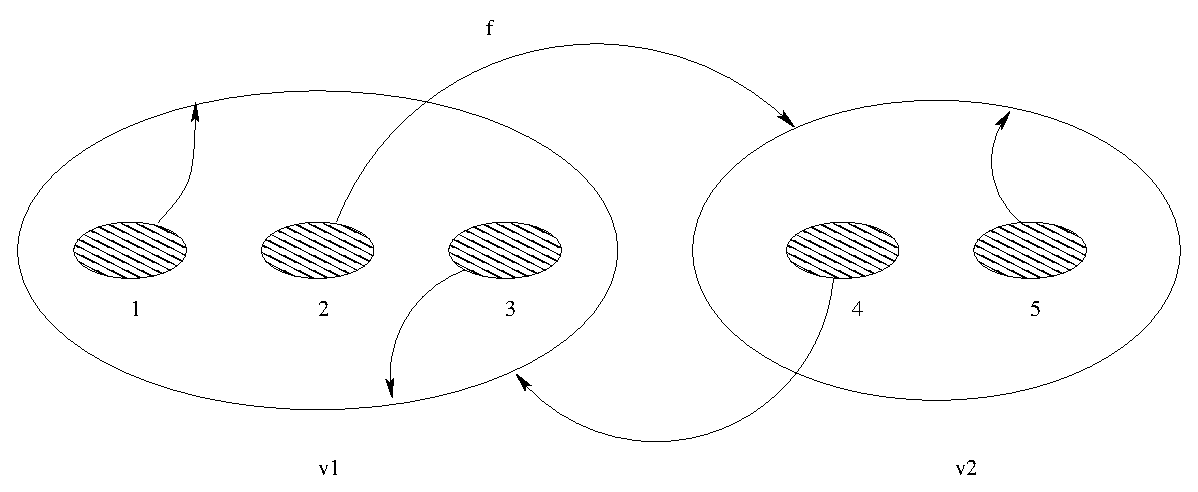
\includegraphics[scale=0.55]{cantor1.eps}
    %  note that the square brace option below is only required
    %  if you intend to produce a list of illustrations
    \caption[Shortened figure caption for the list of illustrations]
      {A Cantor repeller. Long figure captions will be indented left
      and right; short ones will be centred by default.}
    \label{cantor}
\rule[-20pt]{\textwidth}{0.6pt}
\begin{verbatim}
  \begin{figure}
    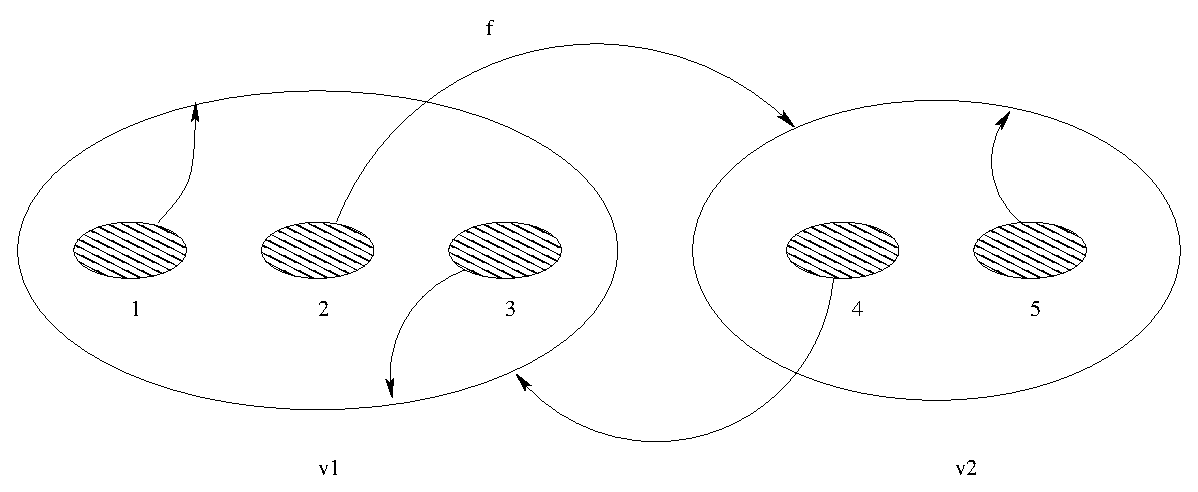
\includegraphics[scale=0.55]{cantor1.eps}
    %  note that the square brace option below is only required
    %  if you intend to produce a list of illustrations
    \caption[Shortened figure caption for the list of illustrations]
      {A Cantor repeller. Long figure captions will be indented left
      and right; short ones will be centred by default.}
    \label{cantor}
  \end{figure}
\end{verbatim}
\rule[20pt]{\textwidth}{0.5pt}
  \end{figure}

\section{Tables}
The \cambridge\ class will cope with most positioning of your tables.
Table captions must be included first, then the label, then the body of the table.
This is illustrated in Table~\ref{sample-table}.
Note that the square brace option below is only required
if you intend to produce a list of tables. You need to use the \verb"minipage"
environment if you have long table captions, or if you have footnotes.

  \begin{table}
    \begin{minipage}{180pt}
    \caption[Shortened table caption for the list of tables]
      {Longer table captions have to be placed inside a minipage,
      otherwise they overhang the table rules.}
    \label{sample-table}
    \addtolength\tabcolsep{2pt}% to stretch columns, if required
      \begin{tabular}{@{}c@{\hspace{25pt}}ccc@{}}
        \hline \hline
        Figure\footnote{\textit{Note:} You must also use a minipage
          environment if you have footnotes.} & $hA$ & $hB$ & $hC$\\
        \hline
        1 & $\exp\left(\pi i\frac58\right)$
          & $\exp\left(\pi i\frac18\right)$ & $0$\\[3pt]
        2 & $-1$    & $\exp\left(\pi i\frac34\right)$ & $1$\\[10pt]
        3 & $-4+3i$ & $-4+3i$ & $\frac74$\\[3pt]
        4 & $-2$    & $-2$    & $\frac54 i$ \\
        \hline \hline
      \end{tabular}
    \end{minipage}
    \rule[-20pt]{\textwidth}{0.5pt}
\begin{verbatim}
  \begin{table}
    \begin{minipage}{180pt}
      %  note that the square brace option below is only required
      %  if you intend to produce a list of tables
    \caption[Shortened table caption for the list of tables]
      {Longer table captions have to be placed inside a minipage,
      otherwise they overhang the table rules.}
    \label{sample-table}
    \addtolength\tabcolsep{2pt}% to stretch columns, if required
      \begin{tabular}{@{}c@{\hspace{25pt}}ccc@{}}
        \hline \hline
        Figure\footnote{\textit{Note:} You must also use a minipage
          environment if you have footnotes.} & $hA$ & $hB$ & $hC$\\
        \hline
        1 & $\exp\left(\pi i\frac58\right)$
          & $\exp\left(\pi i\frac18\right)$ & $0$\\[3pt]
        2 & $-1$    & $\exp\left(\pi i\frac34\right)$ & $1$\\[10pt]
        3 & $-4+3i$ & $-4+3i$ & $\frac74$\\[3pt]
        4 & $-2$    & $-2$    & $\frac54 i$ \\
        \hline \hline
      \end{tabular}
    \end{minipage}
  \end{table}
\end{verbatim}
\rule[20pt]{\textwidth}{0.5pt}
  \end{table}

\subsection{My vertical rules have disappeared}
Vertical rules in tables are not Cambridge house style; {\cambridge}.cls
removes these rules automatically by redefining the \verb"tabular" environment.
Well-organized tables rarely require vertical rules. Where necessary,
grouping can be indicated by the judicious use of extra horizonatal space
(see Section~\ref{addhoriz}). The amended \verb"tabular" also inserts extra
vertical space above and below the horizontal rules produced by \verb"\hline".

Vertical rules can be reinstated, if necessary. Tables will look squashed,
as in the \LaTeX\ book, because the extra vertical space around horizontal
rules will be removed. To reinstate rules globally, add the command
\verb"\reinstaterules" in the preamble; to reinstate rules for an
individual table, place the \verb"\reinstaterules" command
immediately after the relevant \verb"\begin{table}".

The extra space around horizontal rules will also be removed if
you use \verb"array.sty"; you can ignore this effect, because the space
can be reintroduced globally by the typesetters.

\subsection{Adding space between columns}
\label{addhoriz}
You can add space (2pt in this example) between all columns using\linebreak
\verb"\addtolength\tabcolsep{2pt}". If you wanted to expand the space
only between columns~1 and~2, say to~25pt, use
\verb"\begin{tabular}{@{}c@{\hspace{25pt}}ccc@{}}" (see Table~\ref{sample-table}).

\subsection{Adding space between rows}
If you need additional separation between rows (for example,
between rows~2 and~3 in the body of Table~\ref{sample-table}),
adding \verb"[10pt]" immediately after the double backslash at
the end of row~2 will add a 10pt vertical space (the equivalent of
a blank line at this typesize). This method is more controllable
than inserting a horizontal rule.

\section{Landscape figures and tables, using rotating.sty}
Landscape figures and tables are always rotated anticlockwise,
and may be typeset using the \verb"rotating.sty" package with
the \verb"[figuresright]" option. At final make-up stage it is preferable
for landscape pages to fall on verso (left-hand) pages.

In addition to \verb"rotating.sty", include \verb"floatpag.sty" and
the command \verb"\rotfloatpagestyle{empty}". This combination ensures
that headers and footers are removed from the landscape page:
\begin{verbatim}
  \usepackage[figuresright]{rotating}
  \usepackage{floatpag}
  \rotfloatpagestyle{empty}
\end{verbatim}
In some dvi previewers, floats may not appear rotated. If this happens,
you need to convert the dvi file to PostScript or pdf
in order to see the page properly. You can also rotate figures using
the appropriate optional argument in the \verb"\includegraphics" command:
only the illustration is rotated, so running heads are included as usual and captions will
appear at the foot of the figure rather than to the side, both of
which are unsatisfactory in general.

When converting a PostScript file to a pdf file, you may find that
the landscape page comes out upside-down. If this happens, you need
to modify some of the settings in your conversion program.

\subsection{Coding for landscape figures}

Figure~\ref{sidecantor} was produced as follows:
\begin{verbatim}
  \begin{sidewaysfigure}
    \centering
    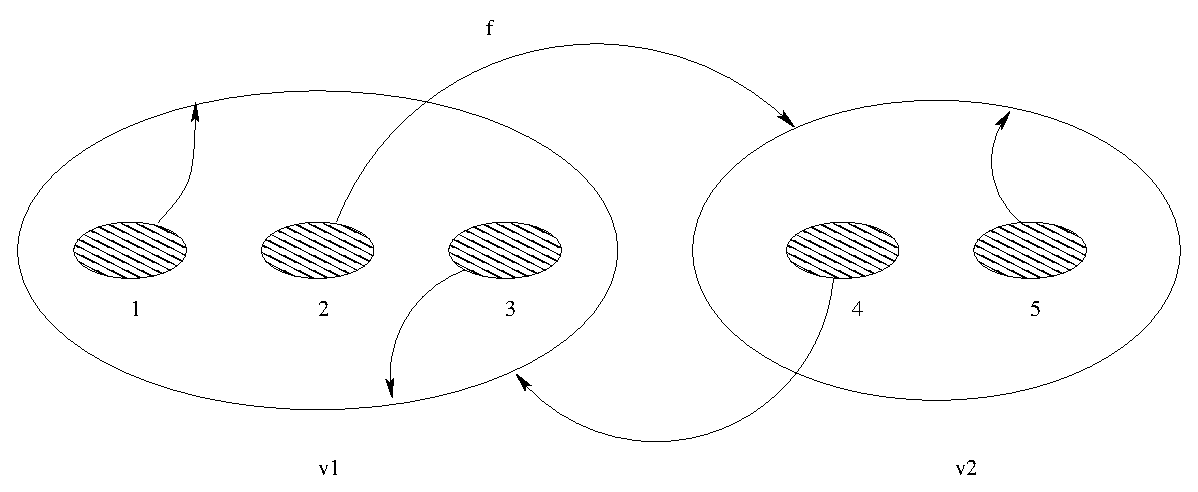
\includegraphics[scale=0.85]{cantor1.eps}
    %  note that the square brace option below is only required
    %  if you intend to produce a list of illustrations
    \caption[Landscape figure]{A Cantor repeller. Figure captions
      will be centred by default.}
    \label{sidecantor}
  \end{sidewaysfigure}
\end{verbatim}
  \begin{sidewaysfigure}
    \centering
    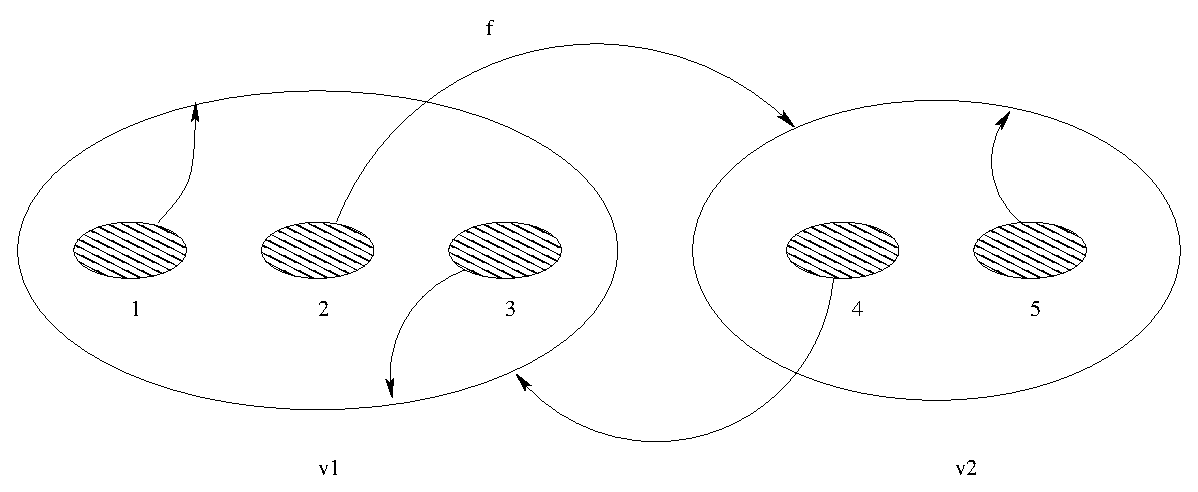
\includegraphics[scale=0.85]{cantor1.eps}
    %  note that the square brace option below is only required
    %  if you intend to produce a list of illustrations
    \caption[Landscape figure]{A Cantor repeller. Figure captions
      will be centred by default.}
    \label{sidecantor}
  \end{sidewaysfigure}


\subsection{Coding for landscape tables}

Table~\ref{sideways} was produced as follows:
%
\begin{smallverbatim}
\begin{sidewaystable}
  \caption[Landscape table]{Grooved ware and beaker features, their finds and
    radiocarbon dates.}
  \label{sideways}
  \addtolength\tabcolsep{-2pt}
  \begin{tabular}{@{}lcccllccccc@{}}
  \hline\hline
  Context & Length & Breadth/  & Depth & Profile & Pottery & Flint & Animal
                                                   & Stone & Other & C14 Dates\\
  && Diameter &&&&& Bones\\[5pt]
  & m & m & m\\
  \hline\\[-5pt]
  \multicolumn{10}{@{}l}{\textbf{Grooved Ware}}\\
  784 & --   & 0.9$\phantom{0}$ &0.18  & Sloping U & P1      & $\times$46
        & $\phantom{0}$$\times$8 && $\times$2 bone & 2150 $\pm$100\,\textsc{bc}\\
  785 & --   & 1.00             &0.12   & Sloping U & P2--4  & $\times$23
                                           & $\times$21 & Hammerstone & -- & --\\
  962 & --   & 1.37             &0.20   & Sloping U & P5--6  & $\times$48
                     & $\times$57 & --& --& 1990 $\pm$80\,\textsc{bc} (Layer 4)\\
  &&&&&&&&&& 1870 $\pm$90\,\textsc{bc} (Layer 1)\\
  983 & 0.83 & 0.73             &0.25   & Stepped U & --     & $\times$18
                                & $\phantom{0}$$\times$8 & -- & Fired clay & --\\
  &&&&&&&&&&\\
  \multicolumn{10}{@{}l}{\textbf{Beaker}}\\
  552 & --   & 0.68             & 0.12  & Saucer    & P7--14 & --           & --
                                                                   & -- &-- &--\\
  790 & --   & 0.60             & 0.25  & U         & P15    & $\times$12   & --
                                                      & Quartzite-lump & -- &--\\
  794 & 2.89 & 0.75             & 0.25  & Irreg.    & P16    & $\phantom{0}$$\times$3
                                                              & -- & -- &-- &--\\
  \hline\hline
  \end{tabular}
\end{sidewaystable}
\end{smallverbatim}
%
\begin{sidewaystable}
  \caption[Landscape table]{Grooved ware and beaker features, their finds and
    radiocarbon dates.}
  \label{sideways}
  \addtolength\tabcolsep{-2pt}
  \begin{tabular}{@{}lcccllccccc@{}}
  \hline\hline
  Context & Length & Breadth/  & Depth & Profile & Pottery & Flint & Animal
                                                   & Stone & Other & C14 Dates\\
  && Diameter &&&&& Bones\\[5pt]
  & m & m & m\\
  \hline\\[-5pt]
  \multicolumn{10}{@{}l}{\textbf{Grooved Ware}}\\
  784 & --   & 0.9$\phantom{0}$ &0.18  & Sloping U & P1      & $\times$46
        & $\phantom{0}$$\times$8 && $\times$2 bone & 2150 $\pm$100\,\textsc{bc}\\
  785 & --   & 1.00             &0.12   & Sloping U & P2--4  & $\times$23
                                           & $\times$21 & Hammerstone & -- & --\\
  962 & --   & 1.37             &0.20   & Sloping U & P5--6  & $\times$48
                     & $\times$57 & --& --& 1990 $\pm$80\,\textsc{bc} (Layer 4)\\
  &&&&&&&&&& 1870 $\pm$90\,\textsc{bc} (Layer 1)\\
  983 & 0.83 & 0.73             &0.25   & Stepped U & --     & $\times$18
                                & $\phantom{0}$$\times$8 & -- & Fired clay & --\\
  &&&&&&&&&&\\
  \multicolumn{10}{@{}l}{\textbf{Beaker}}\\
  552 & --   & 0.68             & 0.12  & Saucer    & P7--14 & --           & --
                                                                   & -- &-- &--\\
  790 & --   & 0.60             & 0.25  & U         & P15    & $\times$12   & --
                                                      & Quartzite-lump & -- &--\\
  794 & 2.89 & 0.75             & 0.25  & Irreg.    & P16    & $\phantom{0}$$\times$3
                                                              & -- & -- &-- &--\\
  \hline\hline
  \end{tabular}%
\end{sidewaystable}

\endinput% Figures and tables
  % 05authored.tex
% 2011/02/28, v3.00 gamma

\chapter{Reference and bibliography lists}
\label{ref}

\section{References and Bibliographies}
Reference lists consist of documents you actually cite in the text; bibliographies
may also list items that are not actually cited so may, for example, contain further reading.
They should be included at the end of the book.
%If you wish to include them at
%the end of chapters instead, or as well, then this can be accommodated with
%a little effort: an example of how to do include references at the ends of
%chapters is given in Section \ref{chapref}.

Reference lists can
be created automatically from a bibliographic database, a \verb".bib" file, or manually; in either instance
you should refer to items in the text using the referencing commands in \LaTeX\
as this will mean your book can be much more easily updated and corrected.

\section{Automatic lists using \textsc{Bib}\upshape{\TeX}}
You will need a \verb".bib" file, a \verb".bst" file that creates a reference
list from that database, and a style file to interpret the commands properly.
For the last, we have chosen to use the natbib package because of its versatility.

First, call in \texttt{natbib.sty}. The bibliographic database for this
guide is called \texttt{percolation.bib};
and we use \texttt{cambridgeauthordate.bst}.
Place the final two commands at the point where you would like the references to appear:
%
\begin{verbatim}
      :
    \usepackage{natbib}
      :
  % \renewcommand{\refname}{Bibliography}
    \bibliography{percolation}
    \bibliographystyle{cambridgeauthordate}
\end{verbatim}
%
Note that by uncommenting the fifth line shown above, you can
change the heading from `References' to `Bibliography'.
Next, \LaTeX\ your book twice. Then run \textsc{Bib}\TeX\ by
executing the command\\[0.5\baselineskip]
\verb"  bibtex "\texttt{\cambridge guide}\\[0.5\baselineskip]
Finally, run your book through \LaTeX\ twice again.
This series of runs will generate a file, the actual reference list,
called \texttt{\cambridge guide.bbl},
which will then be included by \verb"\bibliography{percolation}".

Suppose you have cited 8 entries from the `percolation' database,
e.g. \verb"\citealp{MenshEst}"; \verb"\citealp{Kasymp}"; \verb"\citealp{VGFH}";
\verb"\citealp{HamMaz94}"; \verb"\citealp{HamLower}"; \verb"\citealp{AiBar87}";
\verb"\citealp{MMS}"; and \verb"\citealp{HamAtomBond}";
the output will be just those 8~entries. This guide only cites two items
from the database so only two items are included in the reference list
 (see page~\pageref{refs}).
You can add entries to the list without referring to them
using the \verb"\nocite" command: if you do this the References
should be named as Bibliography.
This guide only cites two items
from the database so only two items are included in the reference list.

\section{Citations using natbib commands}
Here are some of the basic citation commands available with
the natbib package; there are many more if you cannot find what
you need in this list. Bear in mind that Menshikov (1985) or
(Menshikov, 1985) read best, depending on context.\\*[0.5\baselineskip]
\begin{tabular}{@{}ll@{}}
\verb"\citep{MenshEst}"
    & $\rightarrow\enskip$\citep{MenshEst}\\
\verb"\citep[see][p.$\,$34]{MenshEst}"
    & $\rightarrow\enskip$\citep[see][p.$\,$34]{MenshEst}\\
\verb"\citep[e.g.][]{MenshEst}"
    & $\rightarrow\enskip$\citep[e.g.][]{MenshEst}\\
\verb"\citep[Section~2.3]{MenshEst}"
    & $\rightarrow\enskip$\citep[Section~2.3]{MenshEst}\\
\verb"\citep{MenshEst, VGFH}"\\
    & $\hspace{-70pt}\rightarrow\enskip$\citep{MenshEst, VGFH}\\
\verb"\cite{MenshEst, VGFH}"\\
    & $\hspace{-70pt}\rightarrow\enskip$\cite{MenshEst, VGFH}\\
\verb"\citealt{MenshEst}"
    & $\rightarrow\enskip$\citealt{MenshEst}\\
\verb"\cite{MenshEst}"
    & $\rightarrow\enskip$\cite{MenshEst}\\
\verb"\citealp{MenshEst}"
    & $\rightarrow\enskip$\citealp{MenshEst}\\
\verb"\citeauthor{MenshEst}"
    & $\rightarrow\enskip$\citeauthor{MenshEst}\\
\verb"\citeyearpar{MenshEst}"
    & $\rightarrow\enskip$\citeyearpar{MenshEst}\\
\verb"\citeyear{MenshEst}"
    & $\rightarrow\enskip$\citeyear{MenshEst}
\end{tabular}


\subsection{How to change reference entries from author--date to~numbers}
\label{numberedbiblio}

Some authors are used to \verb"\cite{...}" producing a
reference such as~[11] in their manuscripts. If you prefer this style, which
we do not recommend for long lists of references,
use the following option within the natbib package:
\begin{verbatim}
  \usepackage[numbers]{natbib}
\end{verbatim}

\section{Keying in your reference list for an author--date system}
\label{authordatebiblio}

If you are not constructing a list of references from a database,
then the entries need to be keyed as below. Note that if you uncomment
the first line, you can change the heading from `References' to `Bibliography':
%
\begin{smallverbatim}
% \renewcommand{\refname}{Bibliography}
  \begin{thebibliography}{8}
    \expandafter\ifx\csname natexlab\endcsname\relax
      \def\natexlab#1{#1}\fi
    \expandafter\ifx\csname selectlanguage\endcsname\relax
      \def\selectlanguage#1{\relax}\fi

  \bibitem[Aizenman and Barsky, 1987]{AiBar87}
    Aizenman, M., and Barsky, D.~J. 1987.
    Sharpness of the phase transition in percolation models.
    {\em Comm. Math. Phys.}, {\bf 108}, 489--526.

  \bibitem[Hammersley, 1957]{HamLower}
    Hammersley, J.~M. 1957.
    Percolation processes: Lower bounds for the critical probability.
    {\em Ann. Math. Statist.}, {\bf 28}, 790--795.

  \bibitem[Hammersley, 1961]{HamAtomBond}
    Hammersley, J.~M. 1961.
    Comparison of atom and bond percolation processes.
    {\em J. Mathematical Phys.}, {\bf 2}, 728--733.

  \bibitem[Hammersley and Mazzarino, 1994]{HamMaz94}
    Hammersley, J.~M., and Mazzarino, G. 1994.
    Properties of large Eden clusters in the plane.
    {\em Combin. Probab. Comput.}, {\bf 3}, 471--505.

  \bibitem[Kesten, 1990]{Kasymp}
    Kesten, H. 1990.
    Asymptotics in high dimensions for percolation.
    Pages  219--240 of: Grimmett, G.~R., and Welsh, D.~J.~A. (eds),
    {\em Disorder in Physical Systems: A Volume in Honour of John Hammersley}.
    Oxford University Press.

  \bibitem[Menshikov, 1985]{MenshEst}
    Menshikov, M.~V. 1985.
    Estimates for percolation thresholds for lattices in {${\bf R}\sp n$}.
    {\em Dokl. Akad. Nauk SSSR}, {\bf 284}, 36--39.

  \bibitem[Menshikov et~al., 1986]{MMS}
    Menshikov, M.~V., Molchanov, S.~A., and Sidorenko, A.~F. 1986.
    Percolation theory and some applications.
    Pages  53--110 of: {\em Probability theory. Mathematical
    statistics. Theoretical cybernetics, Vol. 24 (Russian)}.
    Akad. Nauk SSSR Vsesoyuz. Inst. Nauchn. i Tekhn. Inform.
    Translated in {\em J. Soviet Math}. {\bf 42} (1988), no. 4,
    1766--1810.

  \bibitem[Vyssotsky et~al., 1961]{VGFH}
    Vyssotsky, V.~A., Gordon, S.~B., Frisch, H.~L., and Hammersley, J.~M. 1961.
    Critical percolation probabilities (bond problem).
    {\em Phys. Rev.}, {\bf 123}, 1566--1567.

  \end{thebibliography}
\end{smallverbatim}

\section{Keying in your reference list for a numbered system}

For this style, you may omit the optional square brace shown
in Section~\ref{authordatebiblio}. Once again, by uncommenting the first line,
you can change the heading from `References' to `Bibliography':
%
\begin{smallverbatim}
% \renewcommand{\refname}{Bibliography}
  \begin{thebibliography}{8}

  \bibitem{AiBar87}
    Aizenman, M., and Barsky, D.~J. 1987.
    Sharpness of the phase transition in percolation models.
    {\em Comm. Math. Phys.}, {\bf 108}, 489--526.
      :
      :
  \bibitem[Vyssotsky et~al., 1961]{VGFH}
    Vyssotsky, V.~A., Gordon, S.~B., Frisch, H.~L., and Hammersley, J.~M. 1961.
    Critical percolation probabilities (bond problem).
    {\em Phys. Rev.}, {\bf 123}, 1566--1567.

  \end{thebibliography}
\end{smallverbatim}

If you add a reference, remember to process \LaTeX\ enough times to get the numbering right in the text.

\section{Including references at the end of chapters}
\label{chapref}

When references are included at the end of chapters, you need to add the command \verb"\chapterreferences", as indicated below. 
In addition, if you wish to change the \textit{References} heading to \textit{References for 
Chapter~\thechapter} (or indeed to something entirely different,
for example \textit{Further Reading}), you can redefine \verb"\refname" as shown:
\begin{verbatim}
  \renewcommand\refname{References for Chapter~\thechapter}
  \chapterreferences
  \bibliography{percolation}\label{refs}
  \bibliographystyle{cambridgeauthordate}
\end{verbatim}

  \renewcommand\refname{References for Chapter~\thechapter}
  \chapterreferences
  \bibliography{percolation}\label{refs}
  \bibliographystyle{cambridgeauthordate}

\section[Including references at the end of chapters \textit{and} at the end of the book]%
  {Including references at the end of chapters \textit{and} at the end of the book
  \sectionmark{References at the end of chapters \textit{and} at the end of the book}}
  \sectionmark{References at the end of chapters \textit{and} at the end of the book}

As illustrated in this guide, add \verb"\bookreferences" immediately before the call 
to the bibliography file. Of course the bibliography file at the end of the book would 
normally be a concatenation of references from the various chapters, but here we are simply using the same one:
\begin{verbatim}
  \renewcommand{\refname}{Bibliography}% if you prefer this heading
  \bookreferences
  \bibliography{percolation}\label{refs}
  \bibliographystyle{cambridgeauthordate}
\end{verbatim}
\endinput% Reference and bibliography lists
  % 06authored.tex
% 2011/02/28, v3.00 gamma

\chapter{Indexes and glossaries}
\label{indexes}

\section{Inserting indexing commands}
You need to code the text so that \LaTeX\ knows what terms to index, and how
to organise them.

If, for example, you have `chocolate cake' in the text, you add this
phrase to the index simply by adding the \verb"\index" command to the source code:
\begin{verbatim}
  ...chocolate cake\index{chocolate cake}
\end{verbatim}
If the text doesn't actually say `chocolate cake', but you want
that in the index, then you should simply type \verb"\index{chocolate cake}" in the source file
at the appropriate point.

\subsection{Subentries}
If your text contained several varieties of cake, you might
also want them listed under `cake' with subentries; to achieve this, use the ! as shown below:
\begin{verbatim}
  ...chocolate cake\index{chocolate cake}\index{cake!chocolate}
  ...lemon cake\index{lemon cake}\index{cake!lemon}
\end{verbatim}
Running the makeindex program (see Section~\ref{makeidx}) will
create an index which contains, in the correct alphabetical order, the following entries:

\vspace{0.5\baselineskip}%
\noindent{\indexsize cake\\
\mbox{}\quad chocolate\\
\mbox{}\quad lemon\\
chocolate cake\\[0.5\baselineskip]
lemon cake\par}

You can also have subsubentries (but there is no support for subsubsubentries):
\begin{verbatim}
  ...Belgian chocolate cake\index{cake!chocolate!Belgian}
\end{verbatim}

\subsection{Page ranges}
If cake appears over several consecutive pages, then the make the first instance:
\begin{verbatim}
  \index{cake|(}
\end{verbatim}
and the final one:
\begin{verbatim}
  \index{cake|)}
\end{verbatim}
When compiled, the index will read (assuming the entries fell on
pages~5 and~10 respectively):\\[0.5\baselineskip]
{\indexsize cake, 5--10}\\[0.5\baselineskip]
The above also works with subentries.

\subsection{Entries without page numbers}
Sometimes you want to add a cross-reference with no page number:
\begin{verbatim}
  ...birthday party\index{cake!orange|see{orange cake}}
\end{verbatim}
will give you:\\[0.5\baselineskip]
{\indexsize cake\\
\mbox{}\quad orange, \textit{see} orange\vadjust{\vspace{3pt}} cake\par}

\subsection{Entries starting with non-alphabetic characters}
If you have index entries in which the first character
is not alphabetical, e.g. \verb"\emph{cake}" or \verb"$\lambda$" you
need to tell \LaTeX\ where to place that word in the final index.
So you would ask for \verb"\emph{cake}" to be sorted as if it
were the word `cake' and \verb"$\lambda$" as if it were the word `lambda'.

The following example shows how to do that
The characters before the \verb"@" symbol in the expression
\verb"lambda@$\lambda$" are for sorting purposes only; what
appears after the symbol is printed in the index. The
character $\lambda$ will appear before lemon cake, since this is what we've requested:
\begin{verbatim}
  ...lemon cake\index{lemon cake}
  ...$\lambda$\index{lambda@$\lambda$}
  ...\emph{cake}\index{cake@\emph{cake}}
\end{verbatim}
The output will be as follows:\\[0.5\baselineskip]
{\indexsize \emph{cake}\\
$\lambda$\\
lemon cake\par}

\section{Creating a single index using makeidx.sty}
\label{makeidx}
The basic \verb"\index" command in \LaTeX\ does not print
anything in its argument but merely `writes' it to a different
file with the extension .idx. (The makeidx programme turns
that into a file with the extension .ind, which is the one in
which all terms are grouped together in alphabetical order,
with all instances and no duplications, i.e. it would
not write 123, 123 against a term in the index.
The .ind file will not change automatically,
even when the .idx file changes: you need to rerun makeidx to change that.) %%BUG: True?

You will need the package makeidx.sty, and the following
commands in the preamble of the root file:\\[0.5\baselineskip]
\verb"  \documentclass{"\texttt{\cambridge}\verb"}"\\
\verb"    \usepackage{makeidx}"\\
\verb"    \makeindex"\\
\verb"    \begin{document}"\\[6.5pt]
%
To generate a single index, normally a subject index, the commands would take the form:
\begin{verbatim}
  \index{diffraction}
  \index{force!hydrodynamic}
  \index{force!interactive}
\end{verbatim}
at the appropriate points in the text.

The command \verb"\printindex" (which outputs the index)
should be placed immediately before the end of the document.
The (optional) \verb"\indextext" command will
insert a phrase below the `Index' chapter heading, across
two columns, the index entries themselves being set in double-column form.

\begin{verbatim}
    \indextext{Page numbers in italics indicate ...}
    \printindex
  \end{document}
\end{verbatim}


Run your files through \LaTeX\ enough times so that the labels, etc.,
are stable. Then execute the command:\\[0.5\baselineskip]
\verb"  makeindex "\texttt{\cambridge test}\\[0.5\baselineskip]
To include the index, you need to run \LaTeX\ one more time.


\section{Creating multiple indexes using multind.sty}
This guide has been prepared using \verb"multind.sty".
This style file redefines the \verb"\makeindex", \verb"\index" and
\verb"\printindex" commands to deal with multiple indexes.

Suppose you want to create an author index and a subject index.
The entries should be in the text as usual, but take the following form:
\begin{verbatim}
  \index{authors}{Young, P.D.F.}
  \index{authors}{Tranah, D.A.}
  \index{authors}{Peterson, K.}
  \index{subject}{diffraction}
  \index{subject}{force!hydrodynamic}
  \index{subject}{force!interactive}
\end{verbatim}
  \index{authors}{Young, P.D.F.}%
  \index{authors}{Tranah, D.A.}%
  \index{authors}{Peterson, K.}%
  \index{subject}{diffraction}%
  \index{subject}{force!hydrodynamic}%
  \index{subject}{force!interactive}%
In the preamble, you need to add the following lines:
\begin{verbatim}
  \usepackage{multind}\ProvidesPackage{multind}
  \makeindex{authors}
  \makeindex{subject}
\end{verbatim}
It is crucial to add the command \verb"\ProvidesPackage{multind}";
this will send a message to the class file to re-style the index into
the \cambridge\ style. You will get a warning in your log file:
\begin{verbatim}
  LaTeX Warning: You have requested package `',
                 but the package provides `multind'.
\end{verbatim}
which can be ignored. At the point where you wish your indexes to appear, you then need the commands:
\begin{verbatim}
  \printindex{authors}{Author index}
  \printindex{subject}{Subject index}
\end{verbatim}
Run your book through \LaTeX\ enough times so that the labels, etc., are stable. Then execute the commands:
\begin{verbatim}
  makeindex authors
  makeindex subject
\end{verbatim}
To include the indexes, you need to run \LaTeX\ one more time.

\section{Warning about index.sty}
This style file also permits multiple indexes.

However, in order to implement \verb"index.sty", it's proved necessary to
modify a number of \LaTeX\ commands seemingly unrelated to indexing,
namely, \verb"\@starttoc", \verb"\raggedbottom", \verb"\flushbottom",
\verb"\addcontents", \verb"\markboth", and \verb"\markright".
Naturally, this could cause incompatibilities between \texttt{index.sty}
and any style files that either redefine these same commands or
make specific assumptions about how they operate.

The redefinition of \verb"\@starttoc" is particularly bad,
since it introduces an incompatibility with the AMS document classes.

For this reason we do not currently recommend using \verb"index.sty".

\enlargethispage{14pt}
\section{Inserting glossary commands}\label{glossary}

You may make use of the glossary.sty style file contained 
within the package http://www.ctan.org/tex-archive/macros/latex/contrib/glossary/.

Briefly, 
you may generate a glossary by inserting the following commands:
%
\begin{verbatim}
\glossary{name={cat},
          description={a domesticated mammal}}

\glossary{name={rabbit},
          description={a rodent, common in the wild or as a pet. Occasionally farmed}}

\glossary{name={dog},
          description={a domesticated mammal, used as a pet or for work purposes}}
\end{verbatim}
where appropriate.
%
\glossary{name={cat},
          description={a domesticated mammal}}

\glossary{name={rabbit},
          description={a rodent, common in the wild or as a pet. Occasionally farmed}}

\glossary{name={dog},
          description={a domesticated mammal, used as a pet or for work purposes}}

You then need to have the following commands in the root file:
\begin{verbatim}
  \usepackage[style=list]{glossary}
  \makeglossary
    :
  \printglossary
\end{verbatim}
(see Appendix~\ref{root} for details). The following example assumes that your 
root file is called tranah.tex. Run the files through \LaTeX, then run the file:
\begin{verbatim}
  makeindex -s tranah.ist -t tranah.glg -o tranah.gls tranah.glo
\end{verbatim}
and finally, run the files through \LaTeX\ again. If you don't want page numbers included (as in this guide)
then add the \verb"number=none" otpional argument, like so:
\begin{verbatim}
  \usepackage[number=none]{glossary}
\end{verbatim}

\endinput
% Indexes
  % 07authored.tex
% 2011/02/28, v3.00 gamma

\chapter{Exercises}
\label{rarities}

\section{Organizing}
Exercises can be handled
in more than one way, as an enunciation or within a list, depending on your style and preference.
They can be scattered through the book, or organised in sets at the end of sections or
chapters, or some combination. But if you mix up styles we strongly recommend
you give the different types different names, for example, Exercises could be
scattered in the text, and Problems could be organised into sets, or vice versa.

\subsection{Scattered through the text --  exer or exer*}
There are two ways of handling exercises scattered through a chapter.
\begin{enumerate}
\item Use amsthm to define an \verb"exer" or \verb"exer*" environment
subject to \verb"\theoremstyle{definition}". See Chapter~\ref{mathchap} for details.
These environments must be defined in the root file for this document.
Exercises created with \verb"exer" are numbered, if at all, in the same sequence as theorems etc.
\item Use the \verb"exerciselist" environment, described below, with a single item.
Exercises created within this environment will be numbered in a
sequence separate from that for theorems etc.

\end{enumerate}

\subsection{At the end of sections -- exerciselist}
The \cambridge\ class file defines the \verb"exerciselist" environment
for setting lists of numbered exercises at the end of sections. These
will not automatically be gathered under a heading, so there will be no  mention of them
in the Table of Contents. Therefore you may wish to list them under a \verb"\subsection"
and set the heading depth appropriately or use the
appropriate \verb"\addcontentsline" command.

There is an option for adding a label such as `Exercise' or `Problem'. The code
\begin{verbatim}
  \begin{exerciselist}[Exercise]
     \item Show that the link between shock formation and
       film rupture is invoked here because of the \ldots
     \item Show that the physical interpretation of \ldots
       \label{physi-ex}
  \end{exerciselist}
\end{verbatim}
will produce
  \begin{exerciselist}[Exercise]
     \item Show that the link between shock formation and
       film rupture is invoked here because of the \ldots
     \item Show that the physical interpretation of \ldots
       \label{physi-ex}
  \end{exerciselist}
Like other numbered environments, individual exercises
(e.g. Exercise~\ref{physi-ex}) can be labeled for automatic cross-referencing.

\subsection{At the end of chapters -- exercises}
If you are gathering all exercises at the end of a given chapter,
use the \verb"exercises" environment rather than \verb"exerciselist". This environment generates an entry
in the table of contents and starts a new unnumbered section and running head. For example,
\begin{verbatim}
  \begin{exercises}
    \item Let the film thickness be $h_0$,
          \begin{equation}
            h=h_0 H{\xi}.
          \label{exerciseeq}
          \end{equation}
          Integrating once, \ldots
    \item Assuming the flow far away from \ldots
  \end{exercises}
\end{verbatim}
will produce (note the mention in the Table of Contents!)
  \begin{exercises}
    \item Let the film thickness be $h_0$,
          \begin{equation}
            h=h_0 H{\xi}.
          \label{exerciseeq}
          \end{equation}
          Integrating once, \ldots
    \item Assuming the flow far away from \ldots
  \end{exercises}
%
If appropriate, you may change the `Exercises' heading to one of the following:
%
\begin{enumerate}[(iii)]
\item `Exercise' -- by using \verb"\begin{exercise}...\end{exercise}"
\item `Problems' -- by using \verb"\begin{problems}...\end{problems}"
\item `Problem' -- by using \verb"\begin{problem}...\end{problem}"
\end{enumerate}
%
For instance,
\begin{verbatim}
  \begin{problems}
    \item By treating $y$ as the independent variable,
          show that the general solution of \ldots
    \item An electrical circuit contains a resistance \ldots
          \label{circuit}
  \end{problems}
\end{verbatim}
will typeset the following:
  \begin{problems}
    \item By treating $y$ as the independent variable,
          show that the general solution of \ldots
    \item An electrical circuit contains a resistance \ldots
          \label{circuit}
  \end{problems}


\endinput
% Exercises

  \backmatter
  \appendix
% if you only have one appendix, use \oneappendix instead of \appendix
  % theorem.tex
% 2011/02/28, v3.00 gamma

\chapter{amsthm commands}
\label{theorem}

You can copy and paste the following code into your root file.
Assuming you have included \verb"amsthm.sty", it will number your theorems,
definitions, etc. in a single sequence within your chapter,
e.g.~Definition~4.1, Lemma~4.2, Lemma~4.3, Proposition~4.4, Corollary~4.5.

\begin{smallverbatim} %don't copy this line!
  \theoremstyle{plain}% default
    \newtheorem{theorem}{Theorem}[chapter]
    \newtheorem{lemma}[theorem]{Lemma}
    \newtheorem{proposition}[theorem]{Proposition}
    \newtheorem{corollary}[theorem]{Corollary}
    \newtheorem{conjecture}[theorem]{Conjecture}

    \newtheorem*{theorem*}{Theorem}
    \newtheorem*{lemma*}{Lemma}
    \newtheorem*{proposition*}{Proposition}
    \newtheorem*{corollary*}{Corollary}
    \newtheorem*{conjecture*}{Conjecture}

  \theoremstyle{definition}
    \newtheorem{definition}[theorem]{Definition}
    \newtheorem{example}[theorem]{Example}
    \newtheorem{prob}[theorem]{Problem}
    \newtheorem{remark}[theorem]{Remark}
    \newtheorem{notation}[theorem]{Notation}
    \newtheorem{exer}[theorem]{Exercise}
    \newtheorem{criterion}[theorem]{Criterion}
    \newtheorem{algorithm}[theorem]{Algorithm}
    \newtheorem{claim}[theorem]{Claim}

    \newtheorem*{definition*}{Definition}
    \newtheorem*{example*}{Example}
    \newtheorem*{prob*}{Problem}
    \newtheorem*{remark*}{Remark}
    \newtheorem*{notation*}{Notation}
    \newtheorem*{exer*}{Exercise}
    \newtheorem*{criterion*}{Criterion}
    \newtheorem*{algorithm*}{Algorithm}
    \newtheorem*{claim*}{Claim}

    \newtheorem*{note}{Note}
    \newtheorem*{summary}{Summary}
    \newtheorem*{acknowledgement}{Acknowledgement}
    \newtheorem*{conclusion}{Conclusion}
\end{smallverbatim} %don't copy this line!

\endinput
  % root.tex
% 2011/06/23, v3.1 gamma

\chapter{The root file for this guide}
\label{root}

\begin{smallverbatim}
% authored_guide.tex
% 2011/06/23, v3.1 gamma
%
% Adapted by Diana Gillooly and David Tranah
% from Ali Woollatt's original documentation for cambridge7A

\NeedsTeXFormat{LaTeX2e}[1996/06/01]

  \documentclass{cambridge7A}
% \documentclass[spanningrule]{../cambridge7A}% option

  \usepackage{natbib}
% \usepackage[numbers]{natbib}% option

  \usepackage[figuresright]{rotating}
  \usepackage{floatpag}
  \rotfloatpagestyle{empty}

% \usepackage{amsmath}% if you are using this package,
                      % it must be loaded before amsthm.sty
  \usepackage{amsthm}
  \usepackage{graphicx}

 \usepackage{txfonts}
% \usepackage[scaled=0.9]{couriers}% use if you're using \tt fonts

% indexes
% uncomment the relevant set of commands

% for a single index
% \usepackage{makeidx}
% \makeindex

% for multiple indexes using multind.sty
  \usepackage{multind}\ProvidesPackage{multind}
  \makeindex{authors}
  \makeindex{subject}

% for glossary entries
  %\usepackage[style=list]{glossary}
  \usepackage[number=none]{glossary}
\makeglossary

% theorem definitions
% see chapter 3 for details
  \theoremstyle{plain}% default
  \newtheorem{theorem}{Theorem}[chapter]
  \newtheorem{lemma}[theorem]{Lemma}
  \newtheorem{proposition}[theorem]{Proposition}
  \newtheorem{corollary}[theorem]{Corollary}
  \newtheorem{conjecture}[theorem]{Conjecture}

  \newtheorem*{theorem*}{Theorem}
  \newtheorem*{lemma*}{Lemma}
  \newtheorem*{proposition*}{Proposition}
  \newtheorem*{corollary*}{Corollary}
  \newtheorem*{conjecture*}{Conjecture}

  \theoremstyle{definition}
  \newtheorem{definition}[theorem]{Definition}
  \newtheorem{example}[theorem]{Example}
  \newtheorem{prob}[theorem]{Problem}
  \newtheorem{remark}[theorem]{Remark}
  \newtheorem{notation}[theorem]{Notation}
  \newtheorem{exer}[theorem]{Exercise}

  \newtheorem*{definition*}{Definition}
  \newtheorem*{example*}{Example}
  \newtheorem*{prob*}{Problem}
  \newtheorem*{remark*}{Remark}
  \newtheorem*{notation*}{Notation}
  \newtheorem*{exer*}{Exercise}

% \hyphenation{docu-ment baseline-skip polar}

% for this documentation, table of contents lists up to subsection level
  \setcounter{tocdepth}{2}

  \newcommand\cambridge{cambridge7A}

% remove the dot and change default for enumerated lists
  \def\makeRRlabeldot#1{\hss\llap{#1}}
  \renewcommand\theenumi{{\rm (\roman{enumi})}}
  \renewcommand\theenumii{{\rm (\alph{enumii})}}
  \renewcommand\theenumiii{{\rm (\arabic{enumiii})}}
  \renewcommand\theenumiv{{\rm (\Alph{enumiv})}}

%%%%%%%%%%%%%%%%%%%%%%%%%%%%%%%%%%%%%

% \includeonly{06authored}

%%%%%%%%%%%%%%%%%%%%%%%%%%%%%%%%%%%%%

\begin{document}

  \title[Subtitle, If You Have One]
    {Preparing Authored Books Using the \cambridge\ Class File}
  \author{Cambridge University Press\\[3\baselineskip]
    This guide was compiled using \hbox{\cambridge.cls \version}\\[\baselineskip]
    The latest version can be downloaded from:
    https://authornet.cambridge.org/information/productionguide/
    LaTeX\_files/\cambridge.zip}

  \bookabstract{This is the guide for authors who are preparing written,
    rather than edited, books.}
  \bookkeywords{\LaTeX; authored books; CUP style; cambridge7A.cls.}

  \frontmatter
  \maketitle
  \tableofcontents
% \listofcontributors

  % author_preface.tex
% 2011/02/28, v3.00 gamma

\chapter*{Preface}
This guide is for authors preparing a book for
Cambridge University Press using \LaTeX\ and the \cambridge\ class
file. It assumes you have some familiarity with \LaTeX\ --
preferably with book.cls, which is itself somewhat different from article.cls.
It is not a substitute for the \LaTeX\ manual itself.


The \cambridge\  class file preserves the standard \LaTeX\ interface,
so any document that can be produced using the standard
{\LaTeX}2e book.cls can also be produced with {\cambridge}.cls.
However, the measure (i.e. width of text) for {\cambridge}.cls
is different from that for book.cls, so
line breaks will change and tables, figures and
long equations may need adjusting if you've already
used book.cls to create a draft.
Commands that differ from the standard \LaTeX\ interface,
or that are provided in addition to the standard interface,
are documented below.

This guide was created by processing the following
(the full root file is in Appendix \ref{root}:
\begin{verbatim}
  \documentclass[spanningrule]{cambridge7A}% options
     \usepackage{natbib}
     \usepackage[figuresright]{rotating}
     \usepackage{floatpag}
     \rotfloatpagestyle{empty}
     \usepackage{amsthm}
     \usepackage{graphicx}
     \usepackage{txfonts}
     \usepackage[scaled=0.9]{couriers}
     \usepackage{multind}\ProvidesPackage{multind}
      :
\end{verbatim}

Even if your book does not use references, rotated items,
computer code, theorems, graphics, or multiple
indexes, it will not hurt to include the packages above.
If you include \verb"multind.sty",
you must also insert \verb"\ProvidesPackage{multind}"; this command sends a message
to the class file to restyle the index into the \cambridge\ style.

Don't use the following standard document class options:
\begin{itemize}
\item \verb"10pt, 11pt, 12pt";
\item \verb"oneside" (\verb"twoside" is the default);
\item \verb"fleqn, leqno, titlepage, twocolumn".
\end{itemize}


\section*{A word about style}
If you so wish, the source files for this guide can be used as templates
for (parts of) your book. It's a really good idea
to observe good programming style -- after all,
\LaTeX\ is a programming language. Make sure for example, that
you list all of your definitions and commands in the preamble,
and that you don't include any that never get used. Don't duplicate them.
Don't use different macros to do the same job. Don't overwrite them
without cause; if you need locally to
\verb"\renewcommand", then make sure you revert back to the original command
as soon as you can.  Make sure the lines in
your root file are short: note there's a difference between line feed and carriage return
in some text editors. Don't include lots of local page make-up commands
unless you're producing final files for printing, or unless you
need to do so for float control. Structure your document
using the environments or commands provided rather than sticking in \verb"\vspace" followed
by some text in bold, for example. Don't number displayed items to which you're not
going to refer. If you are going to refer to things, then use \verb"\label",
\verb"\ref", \verb"\cite", etc. When
you make a decision, document it in the root file, so you can refer back to
it during the writing of your
book  (which can take place over several years!).
For the same reason, keep a style sheet in
which you list things like your hyphenation or capitalization rules.
Most importantly, \emph{be consistent in the way you typeset your book}.

All the above will make the writing, editing, copyediting, correction and reformatting of your
book much more manageable.

\section*{Workflow}
At some stage in the writing of your book, certainly before it's finished, you should discuss
with your CUP editor how the production of your book will be handled. We need to know:
 is the book being prepared
by you in its final design; who is imposing final design or inputting copyeditorial corrections;
when and how will the index be compiled; will the book be printed from final files provided by you;
how competent in \LaTeX\ are you? The answers to these questions will help determine the workflow
your book will follow during production. In any event, before the book is finished,
you should supply your editor with a sample file for evaluating and testing.


Note: books, and chapters,  must carry copyright lines if they are to be
posted on personal or institutional webpages.




  \mainmatter
  \label{partpage}\part{The First Part}
% 01authored.tex
% 2011/02/28, v3.00 gamma

\chapter{Introduction and basic design elements}
\label{intro}

\section{Getting started}
\label{usingcamb}
Copy \cambridge.cls into the correct subdirectory on your system.
To run this guide through \LaTeX,
you need in addition the following style files:\\[0.5\baselineskip]
\verb"    natbib"\\
\verb"    rotating"\\
\verb"    floatpag"\\
\verb"    amsthm"\\
\verb"    graphicx"\\
\verb"    multind"\\[0.5\baselineskip]
If you include \verb"multind.sty", you must also insert the command
\verb"\ProvidesPackage{multind}"; it simply sends a message to the class file
to re-style the index into the \cambridge\ style.

In general, the following standard document class options should \emph{not} be used:
 \begin{itemize}
  \item \texttt{10pt}, \texttt{11pt}, \texttt{12pt};
  \item \texttt{oneside}  (\texttt{twoside} is the default);
  \item \texttt{fleqn}, \texttt{leqno}, \texttt{titlepage}, \texttt{twocolumn}.
 \end{itemize}


\section{Master root file}
Create a master root file for the book. The preamble should begin like so:

\verb"  \documentclass{"\texttt{\cambridge}\verb"}"\\
\verb"    \usepackage{natbib}"\\
\verb"    \usepackage{rotating}"\\
\verb"    \usepackage{floatpag}"\\
\verb"       \rotfloatpagestyle{empty}"\\
\verb"    \usepackage{amsthm}"\\
\verb"    \usepackage{graphicx}"\\
\verb"    \usepackage{txfonts}"\\
\verb"    \usepackage{multind}\ProvidesPackage{multind}"\\[0.5\baselineskip]

In the preamble are specified, for the entire book:
\begin{itemize}
\item font (default\footnote{The default is determined by the class file.
Changes from the default must be specified in the root file.}  = Computer Modern;
this guide is in Times)
\item depth of section numbering (default = three levels)
\item theorem style (no default; must specify)
\item french spacing (default = yes)
\item enumerate style (default = arabic numbered with full stop, but not in this guide)
\item copyright line for the start of each chapter (default = no)
\item spanning rule (default = no, but we include the rule here)
\end{itemize}

The root file for this guide is given in Appendix \ref{root}.

\subsection{Fonts}
Discuss the choice of font with your CUP editor. In most cases, it will be one of the following:
\begin{itemize}
\item Computer Modern (default)
\item mathptmx, available from\\
http://www.ctan.org/tex-archive/fonts/psfonts/psnfss-source/mathptmx/
\item txfonts (chosen for this guide), available from\\
http://www.ctan.org/tex-archive/fonts/txfonts/
\end{itemize}

If you deliver your files in the default Computer Modern font,
we are likely to ask our typesetters to change it to some variety of Times, our preferred font.
However, if your book contains critical line or page breaks (e.g. in reproduced
computer code), we will probably leave it in Computer Modern.
If you typeset in Computer Modern and have computer code in a monospaced font,
we recommend you also use the \verb"couriers.sty" package, as follows:\\[0.5\baselineskip]
\verb"\usepackage[scaled=0.9]{couriers}"\\[0.5\baselineskip]
in order that the code font is comparable in size to the regular text font.

If you deliver your files in either mathptmx or txfonts, we are
unlikely to change the font.

A word about these two font packages: mathptmx changes the default roman font to Adobe Times but does not
support bold math characters. Txfonts does support bold math,
but the kerning of subscripts and superscripts is not ideal and
sometimes requires manual intervention. (N.B. You must load txfonts after amsthm;
otherwise you will get some `already defined' messages.)
We don't give times.sty as an option because it mixes Computer Modern
and Times fonts, and there is a clash between math and italic characters. With txfonts you can get round this clash by using
\verb"$\varv$" instead of \verb"$\mathit{v}$". Another way is to use
 the `upright' lower-case greek characters defined by 
\verb"\nuup", \verb"\alphaup" etc. Thus
$$
\mathit{v},\ \varv,\ \nuup,\ \nu
$$
is produced by
\begin{verbatim}
$$
\mathit{v},\ \varv,\ \nuup,\ \nu
$$
\end{verbatim}


\subsection{Depth of section numbering}
\LaTeX\ provides five levels of section heads. In {\cambridge},
the first three levels are numbered. You can reduce the depth to which
section heads are numbered (please don't increase it).
For example, if you want only sections and subsections numbered,
insert the following in the preamble:
\begin{verbatim}
  \setcounter{secnumdepth}{2}
\end{verbatim}
If you want only sections numbered, change the \verb"{2}" to \verb"{1}".

\subsection{Theorem style}
We use the amsthm package. See Chapter~\ref{mathchap} and amsthdoc,
the documentation for the package.

The theorem syle is specified in the master root file -- among other things,
all enunciations should be numbered in a single sequence, preferably
within each chapter, for ease of navigation. If numbering is getting out of
hand, try numbering enunciations by section rather than by chapter alone.
More details are given in the Section \ref{amsthm}.

\subsection{French spacing}
The  \verb"\frenchspacing" option is chosen by default.
This ensures that no extra space is inserted after full stops.
If you have a strong reason to override this default, key \verb"\nonfrenchspacing" in the preamble.

\subsection{Lists}
The \cambridge\ class provides the following standard list environments:
\begin{itemize}
 \item numbered lists, created using the \verb"enumerate" environment;
 \item bulleted lists, created using the \verb"itemize" environment;
 \item labelled lists, created using the \verb"description" environment.
\end{itemize}
In addition, exercises may be organised into lists; see Chapter \ref{rarities} for details.

The default \verb"enumerate" environment numbers each list item with
an arabic numeral followed by a full stop. You can specify how lists and sublists are `numbered';
for math books we much prefer  (i), (ii), etc. as the top level, as in this guide, so
please cut and paste the following into the preamble of your master root file:\\[0.25\baselineskip]
\begin{verbatim}
\def\makeRRlabeldot#1{\hss\llap{#1}}
\renewcommand\theenumi{{\rm (\roman{enumi})}}
\renewcommand\theenumii{{\rm (\alph{enumii})}}
\renewcommand\theenumiii{{\rm (\arabic{enumiii})}}
\renewcommand\theenumiv{{\rm (\Alph{enumiv})}}
\end{verbatim}
Numbering of lists need not be consistent across the book, but it's attractive if it is. Note that for perfect alignment within the list, you now need to add the width of the widest label in square braces, as shown below. With the above commands included,\\[0.25\baselineskip]
\begin{verbatim}
  \begin{enumerate}[(ii)]
    \item First, the first item \ldots
      \begin{enumerate}[(b)]
        \item First subentry \ldots
        \item Second subentry
      \end{enumerate}
    \item Second, the next item \ldots
      \begin{enumerate}[(b)]
        \item Another subentry
          \begin{enumerate}[(1)]
            \item First subsubentry \ldots
              \begin{enumerate}[(A)]
                \item First subsubsubentry \ldots
              \end{enumerate}
          \end{enumerate}
      \end{enumerate}
  \end{enumerate}
\end{verbatim}
produces the following list:
  \begin{enumerate}[(ii)]
    \item First, the first item \ldots
      \begin{enumerate}[(b)]
        \item First subentry \ldots
        \item Second subentry
      \end{enumerate}
    \item Second, the next item \ldots
      \begin{enumerate}[(b)]
        \item Another subentry
          \begin{enumerate}[(1)]
            \item First subsubentry \ldots
              \begin{enumerate}[(A)]
                \item First subsubsubentry \ldots
              \end{enumerate}
          \end{enumerate}
      \end{enumerate}
  \end{enumerate}

Of course, you can always overide the automatic numbering by including an optional argument, like so: \verb"\item[(I)]", but we'd rather you didn't unless absolutely necessary.

\subsection{Spanning rule at the start of each chapter}
The page design for your book may include `spanning rules' at
start of chapters, between the chapter number and the chapter
title, as in this guide. Spanning rules are obtained as a document class option:
\begin{verbatim}
  \documentclass[spanningrule]{cambridge7A}
\end{verbatim}

\subsection{Abstracts and key words}
Please include in your root file an abstract and key words for the book
using the \verb"\bookabstract" and \verb"\bookkeywords" commands in the body
of the root file: see Appendix~\ref{root} for examples. List up to five key words.
If there is an agreed international classification for your subject, please let us know what it is, and use terms/codes from that. For mathematics books the key words/codes
should be chosen from the 3 digit levels in the 2010 Mathematics Subject classification.
The abstract and key word list might not be printed in the book, but will be associated metadata which will be helpful for users of the electronic version of your book, and in marketing.

In addition, you may add an abstract and key words for individual chapters using \verb"\chapterabstract" and \verb"\chapterkeywords". These will not be printed, but may be useful as metadata (as above).

\subsection{Figures and tables}

The \cambridge\ class will cope with most positioning of your figures and tables.
The \verb"graphicx.sty" package is the recommended way to incorporate figures,
which should be in the form of \verb".eps" files. Convert other figure formats
to this form, rather than compile the book directly to .pdf, as this can produce
platform-dependent output. Each figure should be followed by a caption that
explains what the illustration is about  without having to read the text. The \verb"\caption"
command will also number the figure.

The caption for tables should precede the actual table, but otherwise the same comments apply.

Figures and tables can be set in portrait or landscape (rotated) style. See Chapter \ref{figtabchap}
for further information for more details about figures and tables.

\subsection{Footnotes and endnotes}
Though the \cambridge\ class can accommodate footnotes or endnotes, but not both, we prefer
you to use footnotes.\footnote{Footnotes are arabic numbered, and the counter is reset for each chapter.}

Endnotes are inserted in the text in a similar way to footnotes, but with the \verb"\endnote" command; for example,
\begin{verbatim}
  When the Richardson number\endnote{Lewis Fry Richardson
  (1881--1953).\label{richardson}} increases \ldots
\end{verbatim}
will produce `When the Richardson number$^5$ increases \ldots' in the text --
assuming this is the fifth endnote of the chapter. Use \verb"\theendnotes"  in the root
file to output
 the endnotes at the end of the book, before the references, but after any appendices,
where they will appear, ordered by chapter, in an unnumbered `chapter'.

%\oneappendix
\subsection{Appendices}
Any appendices to your book should be placed immediately before the references,
or endnotes in the event you have them.

\subsubsection{One appendix}
If you have a single appendix, code it as
\begin{verbatim}
 \oneappendix
  \chapter{Appendix}
     :
  \endappendix
\end{verbatim}

\subsubsection{Several appendices}
The following code will generate appendices that are appropriately labeled and named.
\begin{verbatim}
 \appendix
 \chapter{First appendix title}
 \section{Heading}
     :
 \chapter{Second appendix title}
  \section{Heading}
     :
 \endappendix
\end{verbatim}

Equations, theorems etc., tables and figures should be handled exactly as in the main part
of the book. The numbering will be taken care of automatically.
See Appendix \ref{appnum} for examples.

\subsection{References}
Reference lists, or bibliographies, can be at the end of the book
or at the end of chapters, or even both in some cases.
Any of the standard citation styles -- numbered, [12], abbreviated author, [Se],
 or author--date, (Serre 1958), -- are permitted though we prefer the author--date
style, as it's most helpful to readers. Beware of long strings of references
if you switch to this style from a numbered one, and write appropriately to
avoid repeating names. See Chapter \ref{ref} for details.

\subsection{Indexes and Glossaries}
Most books should include an index, usually a subject index. Others may also
include an author index as well. The construction of indexes is usually the responsibility
of the author, and it is advisable to make use of {\LaTeX}'s automatic indexing facility
to create an index before production begins.
See Chapter \ref{indexes} for more information.

You may wish also to include a glossary (they can be helpful in interdisciplinary books)
in which definitions or explanations of key 
ideas are organised alphabetically. See Section \ref{glossary} for more details.

\endinput
% Introduction and basic design elements
  % 02authored.tex
% 2011/02/28, v3.00 gamma

  \chapter{Numbering and headings}
  \label{chapstructure}


\section{Chapter numbering}
Chapter numbers are generated automatically when the full book
is compiled with all chapters in place. Unnumbered chapters, such as the preface,
are specified using the \verb"\chapter*" command.

\section{Section numbering}

\LaTeX\ provides five levels of section heads, and all are defined
in the \cambridge\ class file: \verb"\section", \verb"\subsection",
 \verb"\subsubsection", \verb"\paragraph", and \verb"\subparagraph".
The first three levels are numbered, unless you use a starred version
such as \verb"\section*".

If your book includes an unnumbered chapter (e.g. \verb"\chapter*{Introduction}",
then ensure that all the numbered elements within that chapter
(e.g. section heads, equations, figures, etc) are unnumbered,
by using \verb"\section*{...}" for example.
Otherwise, sections will be numbered 0.1, 0.2, etc.
The same applies to headings subsidiary to an unnumbered section heading,
e.g. subsections, or items that are numbered by section.

\section{Running heads}
In \cambridge\ books, running heads are
\begin{itemize}
\item chapter titles on even-numbered pages (versos), and
\item section numbers (if they exist) and titles  on odd-numbered pages (rectos).
\end{itemize}

If the chapter or section title is long, a shorter version for the running
head can be specified using an optional argument
to the \verb"\chapter" or \verb"\section" command, for example:
\begin{verbatim}
  \chapter[Running head title]{Full chapter title}
\end{verbatim}

To ensure that the full versions of chapter and section titles are
given in the table of contents, simply do the following:

\begin{verbatim}
  \chapter[TOC entry]{Full chapter title}
  \chaptermark{Short title, i.e., running head entry}

  \section[TOC entry]{Full section title
    \sectionmark{Short title, i.e. running head entry}}
    \sectionmark{Short title, i.e. running head entry}
\end{verbatim}
The TOC entry may in fact be the same as the full chapter or section title.
But note that for sections, you need the optional argument to \verb"\section",
even if `TOC entry' is in fact the same text as `Full section title'.
Also, the \verb"\sectionmark" has to be entered twice as shown, because
the first \verb"\sectionmark" deals with the header of the page that
the \verb"\section" command falls on, and the second deals with subsequent pages.
However, there's no need to include section number in the \verb"\sectionmark" argument.

\section{Parts}
Sometimes you may wish break the book into segments that are bigger than chapters. For this
you can use the \verb"\part" command. This will create a Part Title page which will always
appear on an odd-numbered page the verso of which will be blank. An entry of the Table of Contents
will be created automatically: parts are numbered in `words'. For example

\begin{verbatim}
\part{The First Part}
\end{verbatim}

\noindent
produces the Part Title on page \pageref{partpage}. Use max caps for Part Titles, as here.
It's good style to enter Part Titles in the root file. 

\section{Other}
Numbering of other items, such as equations, figures and tables, theorems etc., references, exercises, are
dealt with in relevant chapters.

\endinput% Numbering and headings
  % 03authored.tex
% 2011/02/28, v3.00 gamma

\chapter{Mathematics}
\label{mathchap}

\section{Why are we using amsthm.sty?}\label{amsthm}

Many authors already use \verb"amsthm", so we've made it part of our distribution.
It provides a way of allowing varying types of theorem-like enunciations to
be laid out differently but consistently, and to be numbered automatically within
a numbering system of your choice; and it's easy to implement. To implement it just
include near top of the root file the following lines:\\[0.5\baselineskip]
\verb"  \documentclass{"\texttt{\cambridge}\verb"}"\\
\verb"  \usepackage{amsmath}"\\
\verb"  \usepackage{amsthm}"\\[0.5\baselineskip]
Note that if you are using \verb"amsmath.sty", it \emph{must} precede \verb"amsthm.sty".

Instructions for amsthm.sty are documented separately in \texttt{amsthdoc.pdf}.
We've included \texttt{amsthm.sty} and \texttt{amsthdoc.pdf} in this distribution
for your convenience, but you may find more recent versions on the web.
The following sections discuss basic features, plus a few extras.

To save time, you can copy and paste the code given in Appendix \ref{theorem}
into your root file. This is an extensive list of
theorem-like environments, both numbered and unnumbered.

Our preferred style is that theorems, definitions, remarks, etc. should be numbered in a single
sequence by chapter (so Chapter~4 might have Definition~4.1, Lemma~4.2,
 Lemma~4.3, Proposition~4.4, Example~4.5). This helps navigation.

To do this we used \verb"\newtheorem{theorem}{Theorem}[chapter]".
To number the elements by section, replace \verb"[chapter]" with \verb"[section]".

\section{amsthm styles}
If no \verb"\theoremstyle" command is given in the preamble
of the root file, the style used will be \texttt{plain}.
To specify a different style (we only recommend plan and definition styles),
divide your \verb"\newtheorem" commands
into groups and preface each group with the appropriate \verb"\theoremstyle".

\subsection{amsthm \texttt{plain} style}
The \texttt{plain} style is normally used for theorems, lemmas,
corollaries, propositions, and conjectures. These can be numbered or unnumbered.

\subsection{amsthm \texttt{definition} style}
\label{amsdefn}
The \texttt{definition} style is used for definitions,
remarks, notation, conditions, problems, and examples;
it can also be used for problems and exercises (see Chapter~\ref{rarities}).
These can be numbered or unnumbered.

The example below illustrates the use of both styles, in numbered and unnumbered form.
The code

\begin{verbatim}
  \theoremstyle{plain}% default
  \newtheorem{theorem}{Theorem}[chapter]
  \newtheorem{lemma}[theorem]{Lemma}
  \newtheorem*{corollary*}{Corollary}

  \theoremstyle{definition}
  \newtheorem{definition}[theorem]{Definition}
  \newtheorem{example}[theorem]{Example}

  \begin{theorem}
    Let the scalar function \ldots
  \end{theorem}
  \begin{lemma}[Tranah]
    The first-order free surface amplitudes \ldots
  \end{lemma}
  \begin{definition}
    The series above is the Green function \ldots
  \end{definition}
  \begin{lemma}[\citep{MenshEst}]
    The exotic behaviours of Lagrangian \ldots
  \end{lemma}
  \begin{corollary*}
    Let $G$ be the free group on \ldots
  \end{corollary*}
\end{verbatim}
will produce the following output:
  \begin{theorem}
    Let the scalar function \ldots
  \end{theorem}
  \begin{lemma}[Tranah]
    The first-order free surface amplitudes \ldots
  \end{lemma}
    \begin{definition}
    The series above is the Green function \ldots
  \end{definition}
\begin{lemma}[\citep{MenshEst}]
    The exotic behaviours of Lagrangian \ldots
  \end{lemma}
  \begin{corollary*}
    Let $G$ be the free group on \ldots
  \end{corollary*}
  \begin{definition}
    The correlation between the real and estimated flow \ldots
  \end{definition}
  \begin{example}
    Consider spatial and temporal problems \ldots
  \end{example}


\section{Proofs}
\label{proofs}
The \verb"proof" environment is also part of the
amsthm package and provides a consistent format for proofs.
 For example,
\begin{verbatim}
  \begin{proof}
    Use $K_\lambda$ and $S_\lambda$ to translate combinators
    into $\lambda$-terms. For the converse, translate
    $\lambda x$ \ldots by [$x$] \ldots and use induction
    and the lemma.
  \end{proof}
\end{verbatim}
produces the following:
  \begin{proof}
    Use $K_\lambda$ and $S_\lambda$ to translate combinators
    into $\lambda$-terms. For the converse, translate
    $\lambda x$ \ldots\ by [$x$] \ldots\ and use induction
    and the lemma.
  \end{proof}

\subsection{Adapting the `Proof' heading}
An optional argument allows you to have a different
name from the simple `Proof'. For example, to change the heading
to read `Proof of the Pythagorean Theorem', key the following:
\begin{verbatim}
  \begin{proof}[Proof of the Pythagorean Theorem]
    Start with a generic right-angled triangle \ldots
  \end{proof}
\end{verbatim}
It produces:
  \begin{proof}[Proof of the Pythagorean Theorem]
    Start with a generic right-angled triangle \ldots
  \end{proof}

\subsection{Displayed expressions}
Only number displayed expressions, such as equations, to which you will refer.
Please punctuate all displayed expressions as if they were in-line text.
In multiline displays,
only number the last line (unless you refer to intermediate lines). If you wish
lines on multiline displays to be numbered in a subsequence, either use the \verb"subeqn" environment,
or else use the \verb"\renewcommand", as explained in the \LaTeX\ book, to set up a new sequence,
reverting to the original sequence
when required.  If you wish all the items in a multiline display
to  have the same, single number, centred on the display, use the \verb"array" environment with the
display. Items in appendices are numbered separately. See Appendix \ref{appnum} for an illustration.

The default style is to number equations in one sequence by chapter. If you wish to number by section,
then include the command\\[0.5\baselineskip]
 \verb"\renewcommand\theequation{\arabic{chapter}.\arabic{section}.\arabic{equation}}"\\[0.5\baselineskip]
at the end of the preamble. To illustrate the above, here is a single-line display:
\begin{equation}\label{einstein}
E = Mc^2 .
\end{equation}
Here are examples of a multiline displays:
\begin{equation}
\left.\begin{array}{rcl}
x &=& a+b\\
y &=& c+d\\
z &=& e+f.
\end{array}\right\}
\end{equation}
\begin{eqnarray}
x&=&a+a+b+b\nonumber\\
&=&2a+b+b\nonumber\\
&=&2a+2b.
\end{eqnarray}

\subsection{Typesetting a proof without a \qedsymbol}
Use \verb"proof*"; this is not part of the amsthm package. For example,
\begin{verbatim}
  \begin{proof*}
    The apparent virtual mass coefficient \ldots
  \end{proof*}
\end{verbatim}
produces the following:
  \begin{proof*}
    The apparent virtual mass coefficient \ldots
  \end{proof*}

\subsection{When proofs end with an unnumbered display}
Providing the proof does not end with a numbered display,
you can avoid the \qedsymbol\ dropping onto a following line at the end of a proof
by using \verb"\qedhere":
\begin{verbatim}
  \begin{proof}
    \ldots\ and, as we are all aware,
    \[
       E=mc^2. \qedhere
    \]
  \end{proof}
\end{verbatim}
produces the following:
  \begin{proof}
    \ldots\ and, as we are all aware,
    \[
       E=mc^2. \qedhere
    \]
  \end{proof}
This solution is not part of the amsmath package. When used with amsmath version~2 or later, \verb"\qedhere"
will position \qedsymbol\ flush right; with earlier versions, \qedsymbol\ will be spaced a quad away
from the end of the text or display.

If \verb"\qedhere" produces an error message in an equation, try using \verb"\mbox{\qedhere}" instead.

\subsection{Placing the \qedsymbol\ after an unnumbered displayed eqnarray}
This solution is also not part of the amsmath package. %%BUG? You wrote amsthm here but amsmath above
To enable it, you
need to used the starred version of \verb"proof", and
add both \verb"\arrayqed" and \verb"\arrayqedhere", as shown in the following example:
\begin{verbatim}
  \begin{proof*}
    The following equations prove the theorem:
      \arrayqed
        \begin{eqnarray}
          \epsilon &=& -\frac{1}{2}U_0\frac{\mathrm{d}q'^2}
                       {\mathrm{d}x}\nonumber\\
                   &=& 10\nu\frac{q'^2}{\lambda^2} .
        \arrayqedhere
        \end{eqnarray}
  \end{proof*}
\end{verbatim}
This produces the following:
  \begin{proof*}
    The following equations prove the theorem:
      \arrayqed
        \begin{eqnarray}
          \epsilon &=& -\frac{1}{2}U_0\frac{\mathrm{d}q'^2}
                       {\mathrm{d}x}\nonumber\\
                   &=& 10\nu\frac{q'^2}{\lambda^2} .
        \arrayqedhere
        \end{eqnarray}
  \end{proof*}
Again, the above solution \emph{only} works
if the display is unnumbered.

\endinput
% Mathematics
  % 04authored.tex
% 2011/02/28, v3.00 gamma

\chapter{Figures and tables}
\label{figtabchap}

\section{Figures}

The \cambridge\ class will cope with most positioning of your figures.
As captions fall below figures, the figure must be included first,
then the caption, then the label. This is illustrated in Figure~\ref{cantor}.
The \verb"cantor1.eps" file has been called in using \verb"\usepackage{graphicx}"
in the preamble. Note that if you are producing a list of illustrations
(using \verb"\listoffigures"), you need to repeat the caption
(or place a short version) in square braces, but without the full point.
  \begin{figure}
    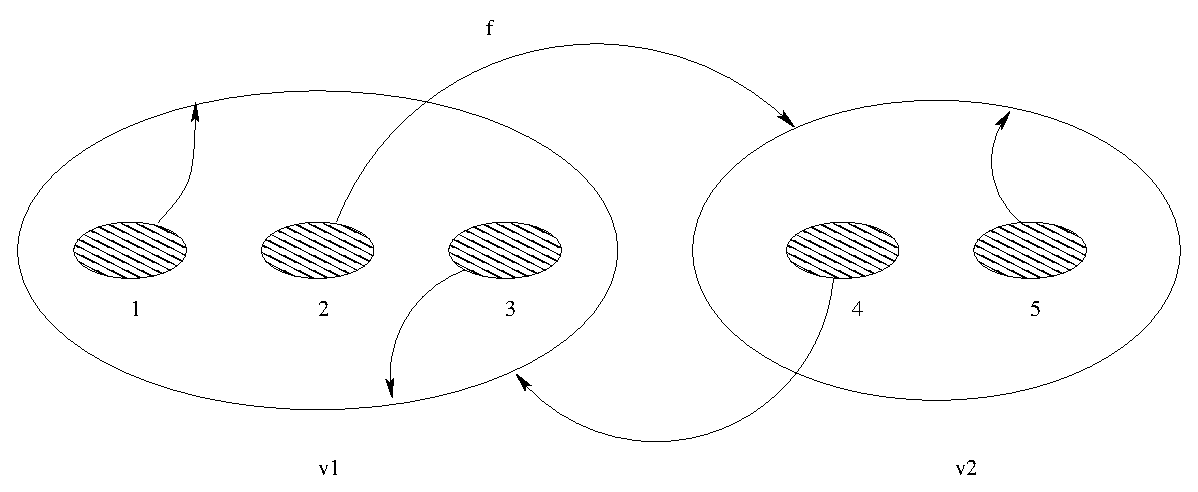
\includegraphics[scale=0.55]{cantor1.eps}
    %  note that the square brace option below is only required
    %  if you intend to produce a list of illustrations
    \caption[Shortened figure caption for the list of illustrations]
      {A Cantor repeller. Long figure captions will be indented left
      and right; short ones will be centred by default.}
    \label{cantor}
\rule[-20pt]{\textwidth}{0.6pt}
\begin{verbatim}
  \begin{figure}
    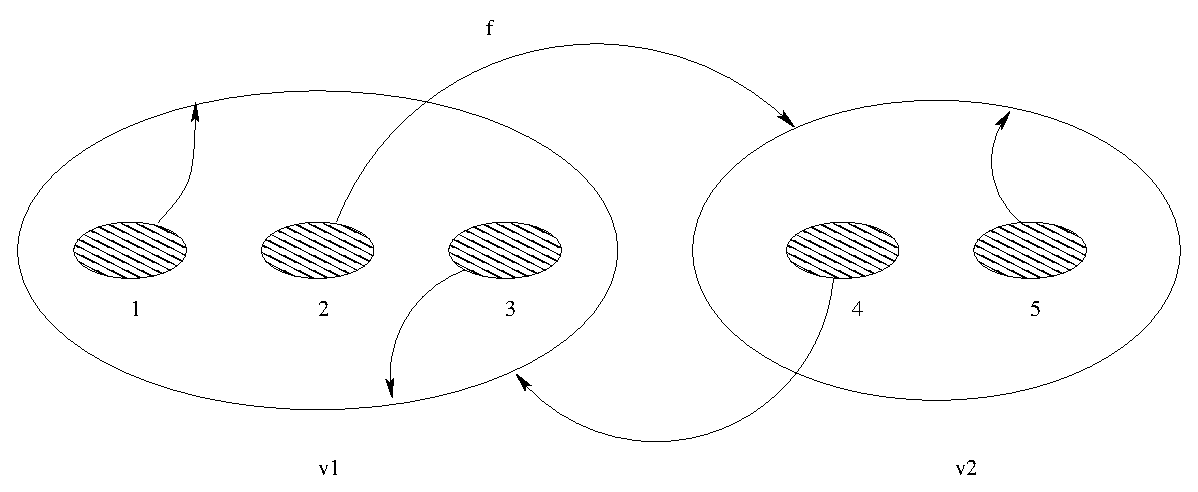
\includegraphics[scale=0.55]{cantor1.eps}
    %  note that the square brace option below is only required
    %  if you intend to produce a list of illustrations
    \caption[Shortened figure caption for the list of illustrations]
      {A Cantor repeller. Long figure captions will be indented left
      and right; short ones will be centred by default.}
    \label{cantor}
  \end{figure}
\end{verbatim}
\rule[20pt]{\textwidth}{0.5pt}
  \end{figure}

\section{Tables}
The \cambridge\ class will cope with most positioning of your tables.
Table captions must be included first, then the label, then the body of the table.
This is illustrated in Table~\ref{sample-table}.
Note that the square brace option below is only required
if you intend to produce a list of tables. You need to use the \verb"minipage"
environment if you have long table captions, or if you have footnotes.

  \begin{table}
    \begin{minipage}{180pt}
    \caption[Shortened table caption for the list of tables]
      {Longer table captions have to be placed inside a minipage,
      otherwise they overhang the table rules.}
    \label{sample-table}
    \addtolength\tabcolsep{2pt}% to stretch columns, if required
      \begin{tabular}{@{}c@{\hspace{25pt}}ccc@{}}
        \hline \hline
        Figure\footnote{\textit{Note:} You must also use a minipage
          environment if you have footnotes.} & $hA$ & $hB$ & $hC$\\
        \hline
        1 & $\exp\left(\pi i\frac58\right)$
          & $\exp\left(\pi i\frac18\right)$ & $0$\\[3pt]
        2 & $-1$    & $\exp\left(\pi i\frac34\right)$ & $1$\\[10pt]
        3 & $-4+3i$ & $-4+3i$ & $\frac74$\\[3pt]
        4 & $-2$    & $-2$    & $\frac54 i$ \\
        \hline \hline
      \end{tabular}
    \end{minipage}
    \rule[-20pt]{\textwidth}{0.5pt}
\begin{verbatim}
  \begin{table}
    \begin{minipage}{180pt}
      %  note that the square brace option below is only required
      %  if you intend to produce a list of tables
    \caption[Shortened table caption for the list of tables]
      {Longer table captions have to be placed inside a minipage,
      otherwise they overhang the table rules.}
    \label{sample-table}
    \addtolength\tabcolsep{2pt}% to stretch columns, if required
      \begin{tabular}{@{}c@{\hspace{25pt}}ccc@{}}
        \hline \hline
        Figure\footnote{\textit{Note:} You must also use a minipage
          environment if you have footnotes.} & $hA$ & $hB$ & $hC$\\
        \hline
        1 & $\exp\left(\pi i\frac58\right)$
          & $\exp\left(\pi i\frac18\right)$ & $0$\\[3pt]
        2 & $-1$    & $\exp\left(\pi i\frac34\right)$ & $1$\\[10pt]
        3 & $-4+3i$ & $-4+3i$ & $\frac74$\\[3pt]
        4 & $-2$    & $-2$    & $\frac54 i$ \\
        \hline \hline
      \end{tabular}
    \end{minipage}
  \end{table}
\end{verbatim}
\rule[20pt]{\textwidth}{0.5pt}
  \end{table}

\subsection{My vertical rules have disappeared}
Vertical rules in tables are not Cambridge house style; {\cambridge}.cls
removes these rules automatically by redefining the \verb"tabular" environment.
Well-organized tables rarely require vertical rules. Where necessary,
grouping can be indicated by the judicious use of extra horizonatal space
(see Section~\ref{addhoriz}). The amended \verb"tabular" also inserts extra
vertical space above and below the horizontal rules produced by \verb"\hline".

Vertical rules can be reinstated, if necessary. Tables will look squashed,
as in the \LaTeX\ book, because the extra vertical space around horizontal
rules will be removed. To reinstate rules globally, add the command
\verb"\reinstaterules" in the preamble; to reinstate rules for an
individual table, place the \verb"\reinstaterules" command
immediately after the relevant \verb"\begin{table}".

The extra space around horizontal rules will also be removed if
you use \verb"array.sty"; you can ignore this effect, because the space
can be reintroduced globally by the typesetters.

\subsection{Adding space between columns}
\label{addhoriz}
You can add space (2pt in this example) between all columns using\linebreak
\verb"\addtolength\tabcolsep{2pt}". If you wanted to expand the space
only between columns~1 and~2, say to~25pt, use
\verb"\begin{tabular}{@{}c@{\hspace{25pt}}ccc@{}}" (see Table~\ref{sample-table}).

\subsection{Adding space between rows}
If you need additional separation between rows (for example,
between rows~2 and~3 in the body of Table~\ref{sample-table}),
adding \verb"[10pt]" immediately after the double backslash at
the end of row~2 will add a 10pt vertical space (the equivalent of
a blank line at this typesize). This method is more controllable
than inserting a horizontal rule.

\section{Landscape figures and tables, using rotating.sty}
Landscape figures and tables are always rotated anticlockwise,
and may be typeset using the \verb"rotating.sty" package with
the \verb"[figuresright]" option. At final make-up stage it is preferable
for landscape pages to fall on verso (left-hand) pages.

In addition to \verb"rotating.sty", include \verb"floatpag.sty" and
the command \verb"\rotfloatpagestyle{empty}". This combination ensures
that headers and footers are removed from the landscape page:
\begin{verbatim}
  \usepackage[figuresright]{rotating}
  \usepackage{floatpag}
  \rotfloatpagestyle{empty}
\end{verbatim}
In some dvi previewers, floats may not appear rotated. If this happens,
you need to convert the dvi file to PostScript or pdf
in order to see the page properly. You can also rotate figures using
the appropriate optional argument in the \verb"\includegraphics" command:
only the illustration is rotated, so running heads are included as usual and captions will
appear at the foot of the figure rather than to the side, both of
which are unsatisfactory in general.

When converting a PostScript file to a pdf file, you may find that
the landscape page comes out upside-down. If this happens, you need
to modify some of the settings in your conversion program.

\subsection{Coding for landscape figures}

Figure~\ref{sidecantor} was produced as follows:
\begin{verbatim}
  \begin{sidewaysfigure}
    \centering
    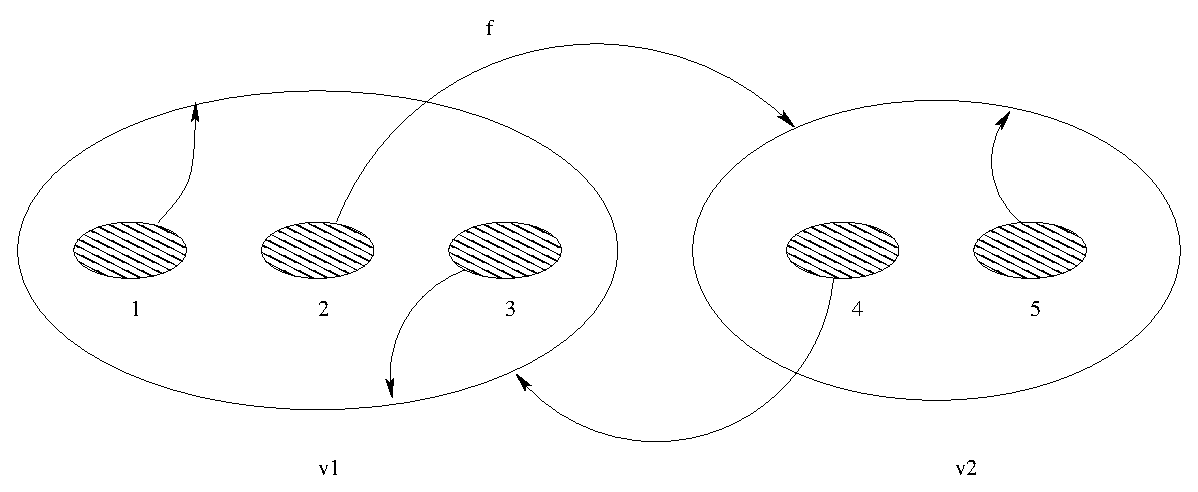
\includegraphics[scale=0.85]{cantor1.eps}
    %  note that the square brace option below is only required
    %  if you intend to produce a list of illustrations
    \caption[Landscape figure]{A Cantor repeller. Figure captions
      will be centred by default.}
    \label{sidecantor}
  \end{sidewaysfigure}
\end{verbatim}
  \begin{sidewaysfigure}
    \centering
    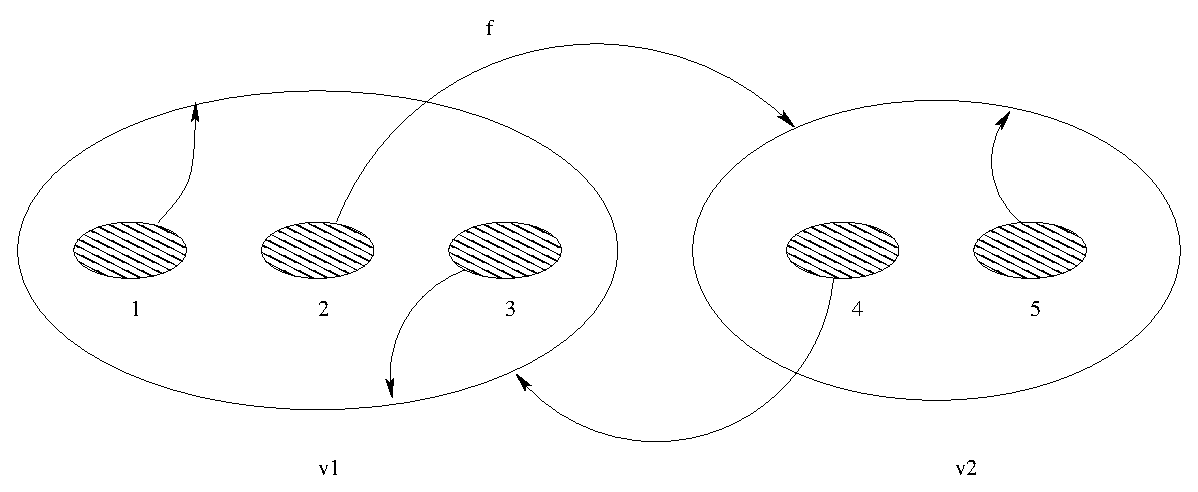
\includegraphics[scale=0.85]{cantor1.eps}
    %  note that the square brace option below is only required
    %  if you intend to produce a list of illustrations
    \caption[Landscape figure]{A Cantor repeller. Figure captions
      will be centred by default.}
    \label{sidecantor}
  \end{sidewaysfigure}


\subsection{Coding for landscape tables}

Table~\ref{sideways} was produced as follows:
%
\begin{smallverbatim}
\begin{sidewaystable}
  \caption[Landscape table]{Grooved ware and beaker features, their finds and
    radiocarbon dates.}
  \label{sideways}
  \addtolength\tabcolsep{-2pt}
  \begin{tabular}{@{}lcccllccccc@{}}
  \hline\hline
  Context & Length & Breadth/  & Depth & Profile & Pottery & Flint & Animal
                                                   & Stone & Other & C14 Dates\\
  && Diameter &&&&& Bones\\[5pt]
  & m & m & m\\
  \hline\\[-5pt]
  \multicolumn{10}{@{}l}{\textbf{Grooved Ware}}\\
  784 & --   & 0.9$\phantom{0}$ &0.18  & Sloping U & P1      & $\times$46
        & $\phantom{0}$$\times$8 && $\times$2 bone & 2150 $\pm$100\,\textsc{bc}\\
  785 & --   & 1.00             &0.12   & Sloping U & P2--4  & $\times$23
                                           & $\times$21 & Hammerstone & -- & --\\
  962 & --   & 1.37             &0.20   & Sloping U & P5--6  & $\times$48
                     & $\times$57 & --& --& 1990 $\pm$80\,\textsc{bc} (Layer 4)\\
  &&&&&&&&&& 1870 $\pm$90\,\textsc{bc} (Layer 1)\\
  983 & 0.83 & 0.73             &0.25   & Stepped U & --     & $\times$18
                                & $\phantom{0}$$\times$8 & -- & Fired clay & --\\
  &&&&&&&&&&\\
  \multicolumn{10}{@{}l}{\textbf{Beaker}}\\
  552 & --   & 0.68             & 0.12  & Saucer    & P7--14 & --           & --
                                                                   & -- &-- &--\\
  790 & --   & 0.60             & 0.25  & U         & P15    & $\times$12   & --
                                                      & Quartzite-lump & -- &--\\
  794 & 2.89 & 0.75             & 0.25  & Irreg.    & P16    & $\phantom{0}$$\times$3
                                                              & -- & -- &-- &--\\
  \hline\hline
  \end{tabular}
\end{sidewaystable}
\end{smallverbatim}
%
\begin{sidewaystable}
  \caption[Landscape table]{Grooved ware and beaker features, their finds and
    radiocarbon dates.}
  \label{sideways}
  \addtolength\tabcolsep{-2pt}
  \begin{tabular}{@{}lcccllccccc@{}}
  \hline\hline
  Context & Length & Breadth/  & Depth & Profile & Pottery & Flint & Animal
                                                   & Stone & Other & C14 Dates\\
  && Diameter &&&&& Bones\\[5pt]
  & m & m & m\\
  \hline\\[-5pt]
  \multicolumn{10}{@{}l}{\textbf{Grooved Ware}}\\
  784 & --   & 0.9$\phantom{0}$ &0.18  & Sloping U & P1      & $\times$46
        & $\phantom{0}$$\times$8 && $\times$2 bone & 2150 $\pm$100\,\textsc{bc}\\
  785 & --   & 1.00             &0.12   & Sloping U & P2--4  & $\times$23
                                           & $\times$21 & Hammerstone & -- & --\\
  962 & --   & 1.37             &0.20   & Sloping U & P5--6  & $\times$48
                     & $\times$57 & --& --& 1990 $\pm$80\,\textsc{bc} (Layer 4)\\
  &&&&&&&&&& 1870 $\pm$90\,\textsc{bc} (Layer 1)\\
  983 & 0.83 & 0.73             &0.25   & Stepped U & --     & $\times$18
                                & $\phantom{0}$$\times$8 & -- & Fired clay & --\\
  &&&&&&&&&&\\
  \multicolumn{10}{@{}l}{\textbf{Beaker}}\\
  552 & --   & 0.68             & 0.12  & Saucer    & P7--14 & --           & --
                                                                   & -- &-- &--\\
  790 & --   & 0.60             & 0.25  & U         & P15    & $\times$12   & --
                                                      & Quartzite-lump & -- &--\\
  794 & 2.89 & 0.75             & 0.25  & Irreg.    & P16    & $\phantom{0}$$\times$3
                                                              & -- & -- &-- &--\\
  \hline\hline
  \end{tabular}%
\end{sidewaystable}

\endinput% Figures and tables
  % 05authored.tex
% 2011/02/28, v3.00 gamma

\chapter{Reference and bibliography lists}
\label{ref}

\section{References and Bibliographies}
Reference lists consist of documents you actually cite in the text; bibliographies
may also list items that are not actually cited so may, for example, contain further reading.
They should be included at the end of the book.
%If you wish to include them at
%the end of chapters instead, or as well, then this can be accommodated with
%a little effort: an example of how to do include references at the ends of
%chapters is given in Section \ref{chapref}.

Reference lists can
be created automatically from a bibliographic database, a \verb".bib" file, or manually; in either instance
you should refer to items in the text using the referencing commands in \LaTeX\
as this will mean your book can be much more easily updated and corrected.

\section{Automatic lists using \textsc{Bib}\upshape{\TeX}}
You will need a \verb".bib" file, a \verb".bst" file that creates a reference
list from that database, and a style file to interpret the commands properly.
For the last, we have chosen to use the natbib package because of its versatility.

First, call in \texttt{natbib.sty}. The bibliographic database for this
guide is called \texttt{percolation.bib};
and we use \texttt{cambridgeauthordate.bst}.
Place the final two commands at the point where you would like the references to appear:
%
\begin{verbatim}
      :
    \usepackage{natbib}
      :
  % \renewcommand{\refname}{Bibliography}
    \bibliography{percolation}
    \bibliographystyle{cambridgeauthordate}
\end{verbatim}
%
Note that by uncommenting the fifth line shown above, you can
change the heading from `References' to `Bibliography'.
Next, \LaTeX\ your book twice. Then run \textsc{Bib}\TeX\ by
executing the command\\[0.5\baselineskip]
\verb"  bibtex "\texttt{\cambridge guide}\\[0.5\baselineskip]
Finally, run your book through \LaTeX\ twice again.
This series of runs will generate a file, the actual reference list,
called \texttt{\cambridge guide.bbl},
which will then be included by \verb"\bibliography{percolation}".

Suppose you have cited 8 entries from the `percolation' database,
e.g. \verb"\citealp{MenshEst}"; \verb"\citealp{Kasymp}"; \verb"\citealp{VGFH}";
\verb"\citealp{HamMaz94}"; \verb"\citealp{HamLower}"; \verb"\citealp{AiBar87}";
\verb"\citealp{MMS}"; and \verb"\citealp{HamAtomBond}";
the output will be just those 8~entries. This guide only cites two items
from the database so only two items are included in the reference list
 (see page~\pageref{refs}).
You can add entries to the list without referring to them
using the \verb"\nocite" command: if you do this the References
should be named as Bibliography.
This guide only cites two items
from the database so only two items are included in the reference list.

\section{Citations using natbib commands}
Here are some of the basic citation commands available with
the natbib package; there are many more if you cannot find what
you need in this list. Bear in mind that Menshikov (1985) or
(Menshikov, 1985) read best, depending on context.\\*[0.5\baselineskip]
\begin{tabular}{@{}ll@{}}
\verb"\citep{MenshEst}"
    & $\rightarrow\enskip$\citep{MenshEst}\\
\verb"\citep[see][p.$\,$34]{MenshEst}"
    & $\rightarrow\enskip$\citep[see][p.$\,$34]{MenshEst}\\
\verb"\citep[e.g.][]{MenshEst}"
    & $\rightarrow\enskip$\citep[e.g.][]{MenshEst}\\
\verb"\citep[Section~2.3]{MenshEst}"
    & $\rightarrow\enskip$\citep[Section~2.3]{MenshEst}\\
\verb"\citep{MenshEst, VGFH}"\\
    & $\hspace{-70pt}\rightarrow\enskip$\citep{MenshEst, VGFH}\\
\verb"\cite{MenshEst, VGFH}"\\
    & $\hspace{-70pt}\rightarrow\enskip$\cite{MenshEst, VGFH}\\
\verb"\citealt{MenshEst}"
    & $\rightarrow\enskip$\citealt{MenshEst}\\
\verb"\cite{MenshEst}"
    & $\rightarrow\enskip$\cite{MenshEst}\\
\verb"\citealp{MenshEst}"
    & $\rightarrow\enskip$\citealp{MenshEst}\\
\verb"\citeauthor{MenshEst}"
    & $\rightarrow\enskip$\citeauthor{MenshEst}\\
\verb"\citeyearpar{MenshEst}"
    & $\rightarrow\enskip$\citeyearpar{MenshEst}\\
\verb"\citeyear{MenshEst}"
    & $\rightarrow\enskip$\citeyear{MenshEst}
\end{tabular}


\subsection{How to change reference entries from author--date to~numbers}
\label{numberedbiblio}

Some authors are used to \verb"\cite{...}" producing a
reference such as~[11] in their manuscripts. If you prefer this style, which
we do not recommend for long lists of references,
use the following option within the natbib package:
\begin{verbatim}
  \usepackage[numbers]{natbib}
\end{verbatim}

\section{Keying in your reference list for an author--date system}
\label{authordatebiblio}

If you are not constructing a list of references from a database,
then the entries need to be keyed as below. Note that if you uncomment
the first line, you can change the heading from `References' to `Bibliography':
%
\begin{smallverbatim}
% \renewcommand{\refname}{Bibliography}
  \begin{thebibliography}{8}
    \expandafter\ifx\csname natexlab\endcsname\relax
      \def\natexlab#1{#1}\fi
    \expandafter\ifx\csname selectlanguage\endcsname\relax
      \def\selectlanguage#1{\relax}\fi

  \bibitem[Aizenman and Barsky, 1987]{AiBar87}
    Aizenman, M., and Barsky, D.~J. 1987.
    Sharpness of the phase transition in percolation models.
    {\em Comm. Math. Phys.}, {\bf 108}, 489--526.

  \bibitem[Hammersley, 1957]{HamLower}
    Hammersley, J.~M. 1957.
    Percolation processes: Lower bounds for the critical probability.
    {\em Ann. Math. Statist.}, {\bf 28}, 790--795.

  \bibitem[Hammersley, 1961]{HamAtomBond}
    Hammersley, J.~M. 1961.
    Comparison of atom and bond percolation processes.
    {\em J. Mathematical Phys.}, {\bf 2}, 728--733.

  \bibitem[Hammersley and Mazzarino, 1994]{HamMaz94}
    Hammersley, J.~M., and Mazzarino, G. 1994.
    Properties of large Eden clusters in the plane.
    {\em Combin. Probab. Comput.}, {\bf 3}, 471--505.

  \bibitem[Kesten, 1990]{Kasymp}
    Kesten, H. 1990.
    Asymptotics in high dimensions for percolation.
    Pages  219--240 of: Grimmett, G.~R., and Welsh, D.~J.~A. (eds),
    {\em Disorder in Physical Systems: A Volume in Honour of John Hammersley}.
    Oxford University Press.

  \bibitem[Menshikov, 1985]{MenshEst}
    Menshikov, M.~V. 1985.
    Estimates for percolation thresholds for lattices in {${\bf R}\sp n$}.
    {\em Dokl. Akad. Nauk SSSR}, {\bf 284}, 36--39.

  \bibitem[Menshikov et~al., 1986]{MMS}
    Menshikov, M.~V., Molchanov, S.~A., and Sidorenko, A.~F. 1986.
    Percolation theory and some applications.
    Pages  53--110 of: {\em Probability theory. Mathematical
    statistics. Theoretical cybernetics, Vol. 24 (Russian)}.
    Akad. Nauk SSSR Vsesoyuz. Inst. Nauchn. i Tekhn. Inform.
    Translated in {\em J. Soviet Math}. {\bf 42} (1988), no. 4,
    1766--1810.

  \bibitem[Vyssotsky et~al., 1961]{VGFH}
    Vyssotsky, V.~A., Gordon, S.~B., Frisch, H.~L., and Hammersley, J.~M. 1961.
    Critical percolation probabilities (bond problem).
    {\em Phys. Rev.}, {\bf 123}, 1566--1567.

  \end{thebibliography}
\end{smallverbatim}

\section{Keying in your reference list for a numbered system}

For this style, you may omit the optional square brace shown
in Section~\ref{authordatebiblio}. Once again, by uncommenting the first line,
you can change the heading from `References' to `Bibliography':
%
\begin{smallverbatim}
% \renewcommand{\refname}{Bibliography}
  \begin{thebibliography}{8}

  \bibitem{AiBar87}
    Aizenman, M., and Barsky, D.~J. 1987.
    Sharpness of the phase transition in percolation models.
    {\em Comm. Math. Phys.}, {\bf 108}, 489--526.
      :
      :
  \bibitem[Vyssotsky et~al., 1961]{VGFH}
    Vyssotsky, V.~A., Gordon, S.~B., Frisch, H.~L., and Hammersley, J.~M. 1961.
    Critical percolation probabilities (bond problem).
    {\em Phys. Rev.}, {\bf 123}, 1566--1567.

  \end{thebibliography}
\end{smallverbatim}

If you add a reference, remember to process \LaTeX\ enough times to get the numbering right in the text.

\section{Including references at the end of chapters}
\label{chapref}

When references are included at the end of chapters, you need to add the command \verb"\chapterreferences", as indicated below. 
In addition, if you wish to change the \textit{References} heading to \textit{References for 
Chapter~\thechapter} (or indeed to something entirely different,
for example \textit{Further Reading}), you can redefine \verb"\refname" as shown:
\begin{verbatim}
  \renewcommand\refname{References for Chapter~\thechapter}
  \chapterreferences
  \bibliography{percolation}\label{refs}
  \bibliographystyle{cambridgeauthordate}
\end{verbatim}

  \renewcommand\refname{References for Chapter~\thechapter}
  \chapterreferences
  \bibliography{percolation}\label{refs}
  \bibliographystyle{cambridgeauthordate}

\section[Including references at the end of chapters \textit{and} at the end of the book]%
  {Including references at the end of chapters \textit{and} at the end of the book
  \sectionmark{References at the end of chapters \textit{and} at the end of the book}}
  \sectionmark{References at the end of chapters \textit{and} at the end of the book}

As illustrated in this guide, add \verb"\bookreferences" immediately before the call 
to the bibliography file. Of course the bibliography file at the end of the book would 
normally be a concatenation of references from the various chapters, but here we are simply using the same one:
\begin{verbatim}
  \renewcommand{\refname}{Bibliography}% if you prefer this heading
  \bookreferences
  \bibliography{percolation}\label{refs}
  \bibliographystyle{cambridgeauthordate}
\end{verbatim}
\endinput% Reference and bibliography lists
  % 06authored.tex
% 2011/02/28, v3.00 gamma

\chapter{Indexes and glossaries}
\label{indexes}

\section{Inserting indexing commands}
You need to code the text so that \LaTeX\ knows what terms to index, and how
to organise them.

If, for example, you have `chocolate cake' in the text, you add this
phrase to the index simply by adding the \verb"\index" command to the source code:
\begin{verbatim}
  ...chocolate cake\index{chocolate cake}
\end{verbatim}
If the text doesn't actually say `chocolate cake', but you want
that in the index, then you should simply type \verb"\index{chocolate cake}" in the source file
at the appropriate point.

\subsection{Subentries}
If your text contained several varieties of cake, you might
also want them listed under `cake' with subentries; to achieve this, use the ! as shown below:
\begin{verbatim}
  ...chocolate cake\index{chocolate cake}\index{cake!chocolate}
  ...lemon cake\index{lemon cake}\index{cake!lemon}
\end{verbatim}
Running the makeindex program (see Section~\ref{makeidx}) will
create an index which contains, in the correct alphabetical order, the following entries:

\vspace{0.5\baselineskip}%
\noindent{\indexsize cake\\
\mbox{}\quad chocolate\\
\mbox{}\quad lemon\\
chocolate cake\\[0.5\baselineskip]
lemon cake\par}

You can also have subsubentries (but there is no support for subsubsubentries):
\begin{verbatim}
  ...Belgian chocolate cake\index{cake!chocolate!Belgian}
\end{verbatim}

\subsection{Page ranges}
If cake appears over several consecutive pages, then the make the first instance:
\begin{verbatim}
  \index{cake|(}
\end{verbatim}
and the final one:
\begin{verbatim}
  \index{cake|)}
\end{verbatim}
When compiled, the index will read (assuming the entries fell on
pages~5 and~10 respectively):\\[0.5\baselineskip]
{\indexsize cake, 5--10}\\[0.5\baselineskip]
The above also works with subentries.

\subsection{Entries without page numbers}
Sometimes you want to add a cross-reference with no page number:
\begin{verbatim}
  ...birthday party\index{cake!orange|see{orange cake}}
\end{verbatim}
will give you:\\[0.5\baselineskip]
{\indexsize cake\\
\mbox{}\quad orange, \textit{see} orange\vadjust{\vspace{3pt}} cake\par}

\subsection{Entries starting with non-alphabetic characters}
If you have index entries in which the first character
is not alphabetical, e.g. \verb"\emph{cake}" or \verb"$\lambda$" you
need to tell \LaTeX\ where to place that word in the final index.
So you would ask for \verb"\emph{cake}" to be sorted as if it
were the word `cake' and \verb"$\lambda$" as if it were the word `lambda'.

The following example shows how to do that
The characters before the \verb"@" symbol in the expression
\verb"lambda@$\lambda$" are for sorting purposes only; what
appears after the symbol is printed in the index. The
character $\lambda$ will appear before lemon cake, since this is what we've requested:
\begin{verbatim}
  ...lemon cake\index{lemon cake}
  ...$\lambda$\index{lambda@$\lambda$}
  ...\emph{cake}\index{cake@\emph{cake}}
\end{verbatim}
The output will be as follows:\\[0.5\baselineskip]
{\indexsize \emph{cake}\\
$\lambda$\\
lemon cake\par}

\section{Creating a single index using makeidx.sty}
\label{makeidx}
The basic \verb"\index" command in \LaTeX\ does not print
anything in its argument but merely `writes' it to a different
file with the extension .idx. (The makeidx programme turns
that into a file with the extension .ind, which is the one in
which all terms are grouped together in alphabetical order,
with all instances and no duplications, i.e. it would
not write 123, 123 against a term in the index.
The .ind file will not change automatically,
even when the .idx file changes: you need to rerun makeidx to change that.) %%BUG: True?

You will need the package makeidx.sty, and the following
commands in the preamble of the root file:\\[0.5\baselineskip]
\verb"  \documentclass{"\texttt{\cambridge}\verb"}"\\
\verb"    \usepackage{makeidx}"\\
\verb"    \makeindex"\\
\verb"    \begin{document}"\\[6.5pt]
%
To generate a single index, normally a subject index, the commands would take the form:
\begin{verbatim}
  \index{diffraction}
  \index{force!hydrodynamic}
  \index{force!interactive}
\end{verbatim}
at the appropriate points in the text.

The command \verb"\printindex" (which outputs the index)
should be placed immediately before the end of the document.
The (optional) \verb"\indextext" command will
insert a phrase below the `Index' chapter heading, across
two columns, the index entries themselves being set in double-column form.

\begin{verbatim}
    \indextext{Page numbers in italics indicate ...}
    \printindex
  \end{document}
\end{verbatim}


Run your files through \LaTeX\ enough times so that the labels, etc.,
are stable. Then execute the command:\\[0.5\baselineskip]
\verb"  makeindex "\texttt{\cambridge test}\\[0.5\baselineskip]
To include the index, you need to run \LaTeX\ one more time.


\section{Creating multiple indexes using multind.sty}
This guide has been prepared using \verb"multind.sty".
This style file redefines the \verb"\makeindex", \verb"\index" and
\verb"\printindex" commands to deal with multiple indexes.

Suppose you want to create an author index and a subject index.
The entries should be in the text as usual, but take the following form:
\begin{verbatim}
  \index{authors}{Young, P.D.F.}
  \index{authors}{Tranah, D.A.}
  \index{authors}{Peterson, K.}
  \index{subject}{diffraction}
  \index{subject}{force!hydrodynamic}
  \index{subject}{force!interactive}
\end{verbatim}
  \index{authors}{Young, P.D.F.}%
  \index{authors}{Tranah, D.A.}%
  \index{authors}{Peterson, K.}%
  \index{subject}{diffraction}%
  \index{subject}{force!hydrodynamic}%
  \index{subject}{force!interactive}%
In the preamble, you need to add the following lines:
\begin{verbatim}
  \usepackage{multind}\ProvidesPackage{multind}
  \makeindex{authors}
  \makeindex{subject}
\end{verbatim}
It is crucial to add the command \verb"\ProvidesPackage{multind}";
this will send a message to the class file to re-style the index into
the \cambridge\ style. You will get a warning in your log file:
\begin{verbatim}
  LaTeX Warning: You have requested package `',
                 but the package provides `multind'.
\end{verbatim}
which can be ignored. At the point where you wish your indexes to appear, you then need the commands:
\begin{verbatim}
  \printindex{authors}{Author index}
  \printindex{subject}{Subject index}
\end{verbatim}
Run your book through \LaTeX\ enough times so that the labels, etc., are stable. Then execute the commands:
\begin{verbatim}
  makeindex authors
  makeindex subject
\end{verbatim}
To include the indexes, you need to run \LaTeX\ one more time.

\section{Warning about index.sty}
This style file also permits multiple indexes.

However, in order to implement \verb"index.sty", it's proved necessary to
modify a number of \LaTeX\ commands seemingly unrelated to indexing,
namely, \verb"\@starttoc", \verb"\raggedbottom", \verb"\flushbottom",
\verb"\addcontents", \verb"\markboth", and \verb"\markright".
Naturally, this could cause incompatibilities between \texttt{index.sty}
and any style files that either redefine these same commands or
make specific assumptions about how they operate.

The redefinition of \verb"\@starttoc" is particularly bad,
since it introduces an incompatibility with the AMS document classes.

For this reason we do not currently recommend using \verb"index.sty".

\enlargethispage{14pt}
\section{Inserting glossary commands}\label{glossary}

You may make use of the glossary.sty style file contained 
within the package http://www.ctan.org/tex-archive/macros/latex/contrib/glossary/.

Briefly, 
you may generate a glossary by inserting the following commands:
%
\begin{verbatim}
\glossary{name={cat},
          description={a domesticated mammal}}

\glossary{name={rabbit},
          description={a rodent, common in the wild or as a pet. Occasionally farmed}}

\glossary{name={dog},
          description={a domesticated mammal, used as a pet or for work purposes}}
\end{verbatim}
where appropriate.
%
\glossary{name={cat},
          description={a domesticated mammal}}

\glossary{name={rabbit},
          description={a rodent, common in the wild or as a pet. Occasionally farmed}}

\glossary{name={dog},
          description={a domesticated mammal, used as a pet or for work purposes}}

You then need to have the following commands in the root file:
\begin{verbatim}
  \usepackage[style=list]{glossary}
  \makeglossary
    :
  \printglossary
\end{verbatim}
(see Appendix~\ref{root} for details). The following example assumes that your 
root file is called tranah.tex. Run the files through \LaTeX, then run the file:
\begin{verbatim}
  makeindex -s tranah.ist -t tranah.glg -o tranah.gls tranah.glo
\end{verbatim}
and finally, run the files through \LaTeX\ again. If you don't want page numbers included (as in this guide)
then add the \verb"number=none" otpional argument, like so:
\begin{verbatim}
  \usepackage[number=none]{glossary}
\end{verbatim}

\endinput
% Indexes
  % 07authored.tex
% 2011/02/28, v3.00 gamma

\chapter{Exercises}
\label{rarities}

\section{Organizing}
Exercises can be handled
in more than one way, as an enunciation or within a list, depending on your style and preference.
They can be scattered through the book, or organised in sets at the end of sections or
chapters, or some combination. But if you mix up styles we strongly recommend
you give the different types different names, for example, Exercises could be
scattered in the text, and Problems could be organised into sets, or vice versa.

\subsection{Scattered through the text --  exer or exer*}
There are two ways of handling exercises scattered through a chapter.
\begin{enumerate}
\item Use amsthm to define an \verb"exer" or \verb"exer*" environment
subject to \verb"\theoremstyle{definition}". See Chapter~\ref{mathchap} for details.
These environments must be defined in the root file for this document.
Exercises created with \verb"exer" are numbered, if at all, in the same sequence as theorems etc.
\item Use the \verb"exerciselist" environment, described below, with a single item.
Exercises created within this environment will be numbered in a
sequence separate from that for theorems etc.

\end{enumerate}

\subsection{At the end of sections -- exerciselist}
The \cambridge\ class file defines the \verb"exerciselist" environment
for setting lists of numbered exercises at the end of sections. These
will not automatically be gathered under a heading, so there will be no  mention of them
in the Table of Contents. Therefore you may wish to list them under a \verb"\subsection"
and set the heading depth appropriately or use the
appropriate \verb"\addcontentsline" command.

There is an option for adding a label such as `Exercise' or `Problem'. The code
\begin{verbatim}
  \begin{exerciselist}[Exercise]
     \item Show that the link between shock formation and
       film rupture is invoked here because of the \ldots
     \item Show that the physical interpretation of \ldots
       \label{physi-ex}
  \end{exerciselist}
\end{verbatim}
will produce
  \begin{exerciselist}[Exercise]
     \item Show that the link between shock formation and
       film rupture is invoked here because of the \ldots
     \item Show that the physical interpretation of \ldots
       \label{physi-ex}
  \end{exerciselist}
Like other numbered environments, individual exercises
(e.g. Exercise~\ref{physi-ex}) can be labeled for automatic cross-referencing.

\subsection{At the end of chapters -- exercises}
If you are gathering all exercises at the end of a given chapter,
use the \verb"exercises" environment rather than \verb"exerciselist". This environment generates an entry
in the table of contents and starts a new unnumbered section and running head. For example,
\begin{verbatim}
  \begin{exercises}
    \item Let the film thickness be $h_0$,
          \begin{equation}
            h=h_0 H{\xi}.
          \label{exerciseeq}
          \end{equation}
          Integrating once, \ldots
    \item Assuming the flow far away from \ldots
  \end{exercises}
\end{verbatim}
will produce (note the mention in the Table of Contents!)
  \begin{exercises}
    \item Let the film thickness be $h_0$,
          \begin{equation}
            h=h_0 H{\xi}.
          \label{exerciseeq}
          \end{equation}
          Integrating once, \ldots
    \item Assuming the flow far away from \ldots
  \end{exercises}
%
If appropriate, you may change the `Exercises' heading to one of the following:
%
\begin{enumerate}[(iii)]
\item `Exercise' -- by using \verb"\begin{exercise}...\end{exercise}"
\item `Problems' -- by using \verb"\begin{problems}...\end{problems}"
\item `Problem' -- by using \verb"\begin{problem}...\end{problem}"
\end{enumerate}
%
For instance,
\begin{verbatim}
  \begin{problems}
    \item By treating $y$ as the independent variable,
          show that the general solution of \ldots
    \item An electrical circuit contains a resistance \ldots
          \label{circuit}
  \end{problems}
\end{verbatim}
will typeset the following:
  \begin{problems}
    \item By treating $y$ as the independent variable,
          show that the general solution of \ldots
    \item An electrical circuit contains a resistance \ldots
          \label{circuit}
  \end{problems}


\endinput
% Exercises

  \backmatter
  \appendix
% if you only have one appendix, use \oneappendix instead of \appendix
  % theorem.tex
% 2011/02/28, v3.00 gamma

\chapter{amsthm commands}
\label{theorem}

You can copy and paste the following code into your root file.
Assuming you have included \verb"amsthm.sty", it will number your theorems,
definitions, etc. in a single sequence within your chapter,
e.g.~Definition~4.1, Lemma~4.2, Lemma~4.3, Proposition~4.4, Corollary~4.5.

\begin{smallverbatim} %don't copy this line!
  \theoremstyle{plain}% default
    \newtheorem{theorem}{Theorem}[chapter]
    \newtheorem{lemma}[theorem]{Lemma}
    \newtheorem{proposition}[theorem]{Proposition}
    \newtheorem{corollary}[theorem]{Corollary}
    \newtheorem{conjecture}[theorem]{Conjecture}

    \newtheorem*{theorem*}{Theorem}
    \newtheorem*{lemma*}{Lemma}
    \newtheorem*{proposition*}{Proposition}
    \newtheorem*{corollary*}{Corollary}
    \newtheorem*{conjecture*}{Conjecture}

  \theoremstyle{definition}
    \newtheorem{definition}[theorem]{Definition}
    \newtheorem{example}[theorem]{Example}
    \newtheorem{prob}[theorem]{Problem}
    \newtheorem{remark}[theorem]{Remark}
    \newtheorem{notation}[theorem]{Notation}
    \newtheorem{exer}[theorem]{Exercise}
    \newtheorem{criterion}[theorem]{Criterion}
    \newtheorem{algorithm}[theorem]{Algorithm}
    \newtheorem{claim}[theorem]{Claim}

    \newtheorem*{definition*}{Definition}
    \newtheorem*{example*}{Example}
    \newtheorem*{prob*}{Problem}
    \newtheorem*{remark*}{Remark}
    \newtheorem*{notation*}{Notation}
    \newtheorem*{exer*}{Exercise}
    \newtheorem*{criterion*}{Criterion}
    \newtheorem*{algorithm*}{Algorithm}
    \newtheorem*{claim*}{Claim}

    \newtheorem*{note}{Note}
    \newtheorem*{summary}{Summary}
    \newtheorem*{acknowledgement}{Acknowledgement}
    \newtheorem*{conclusion}{Conclusion}
\end{smallverbatim} %don't copy this line!

\endinput
  % root.tex
% 2011/06/23, v3.1 gamma

\chapter{The root file for this guide}
\label{root}

\begin{smallverbatim}
% authored_guide.tex
% 2011/06/23, v3.1 gamma
%
% Adapted by Diana Gillooly and David Tranah
% from Ali Woollatt's original documentation for cambridge7A

\NeedsTeXFormat{LaTeX2e}[1996/06/01]

  \documentclass{cambridge7A}
% \documentclass[spanningrule]{../cambridge7A}% option

  \usepackage{natbib}
% \usepackage[numbers]{natbib}% option

  \usepackage[figuresright]{rotating}
  \usepackage{floatpag}
  \rotfloatpagestyle{empty}

% \usepackage{amsmath}% if you are using this package,
                      % it must be loaded before amsthm.sty
  \usepackage{amsthm}
  \usepackage{graphicx}

 \usepackage{txfonts}
% \usepackage[scaled=0.9]{couriers}% use if you're using \tt fonts

% indexes
% uncomment the relevant set of commands

% for a single index
% \usepackage{makeidx}
% \makeindex

% for multiple indexes using multind.sty
  \usepackage{multind}\ProvidesPackage{multind}
  \makeindex{authors}
  \makeindex{subject}

% for glossary entries
  %\usepackage[style=list]{glossary}
  \usepackage[number=none]{glossary}
\makeglossary

% theorem definitions
% see chapter 3 for details
  \theoremstyle{plain}% default
  \newtheorem{theorem}{Theorem}[chapter]
  \newtheorem{lemma}[theorem]{Lemma}
  \newtheorem{proposition}[theorem]{Proposition}
  \newtheorem{corollary}[theorem]{Corollary}
  \newtheorem{conjecture}[theorem]{Conjecture}

  \newtheorem*{theorem*}{Theorem}
  \newtheorem*{lemma*}{Lemma}
  \newtheorem*{proposition*}{Proposition}
  \newtheorem*{corollary*}{Corollary}
  \newtheorem*{conjecture*}{Conjecture}

  \theoremstyle{definition}
  \newtheorem{definition}[theorem]{Definition}
  \newtheorem{example}[theorem]{Example}
  \newtheorem{prob}[theorem]{Problem}
  \newtheorem{remark}[theorem]{Remark}
  \newtheorem{notation}[theorem]{Notation}
  \newtheorem{exer}[theorem]{Exercise}

  \newtheorem*{definition*}{Definition}
  \newtheorem*{example*}{Example}
  \newtheorem*{prob*}{Problem}
  \newtheorem*{remark*}{Remark}
  \newtheorem*{notation*}{Notation}
  \newtheorem*{exer*}{Exercise}

% \hyphenation{docu-ment baseline-skip polar}

% for this documentation, table of contents lists up to subsection level
  \setcounter{tocdepth}{2}

  \newcommand\cambridge{cambridge7A}

% remove the dot and change default for enumerated lists
  \def\makeRRlabeldot#1{\hss\llap{#1}}
  \renewcommand\theenumi{{\rm (\roman{enumi})}}
  \renewcommand\theenumii{{\rm (\alph{enumii})}}
  \renewcommand\theenumiii{{\rm (\arabic{enumiii})}}
  \renewcommand\theenumiv{{\rm (\Alph{enumiv})}}

%%%%%%%%%%%%%%%%%%%%%%%%%%%%%%%%%%%%%

% \includeonly{06authored}

%%%%%%%%%%%%%%%%%%%%%%%%%%%%%%%%%%%%%

\begin{document}

  \title[Subtitle, If You Have One]
    {Preparing Authored Books Using the \cambridge\ Class File}
  \author{Cambridge University Press\\[3\baselineskip]
    This guide was compiled using \hbox{\cambridge.cls \version}\\[\baselineskip]
    The latest version can be downloaded from:
    https://authornet.cambridge.org/information/productionguide/
    LaTeX\_files/\cambridge.zip}

  \bookabstract{This is the guide for authors who are preparing written,
    rather than edited, books.}
  \bookkeywords{\LaTeX; authored books; CUP style; cambridge7A.cls.}

  \frontmatter
  \maketitle
  \tableofcontents
% \listofcontributors

  % author_preface.tex
% 2011/02/28, v3.00 gamma

\chapter*{Preface}
This guide is for authors preparing a book for
Cambridge University Press using \LaTeX\ and the \cambridge\ class
file. It assumes you have some familiarity with \LaTeX\ --
preferably with book.cls, which is itself somewhat different from article.cls.
It is not a substitute for the \LaTeX\ manual itself.


The \cambridge\  class file preserves the standard \LaTeX\ interface,
so any document that can be produced using the standard
{\LaTeX}2e book.cls can also be produced with {\cambridge}.cls.
However, the measure (i.e. width of text) for {\cambridge}.cls
is different from that for book.cls, so
line breaks will change and tables, figures and
long equations may need adjusting if you've already
used book.cls to create a draft.
Commands that differ from the standard \LaTeX\ interface,
or that are provided in addition to the standard interface,
are documented below.

This guide was created by processing the following
(the full root file is in Appendix \ref{root}:
\begin{verbatim}
  \documentclass[spanningrule]{cambridge7A}% options
     \usepackage{natbib}
     \usepackage[figuresright]{rotating}
     \usepackage{floatpag}
     \rotfloatpagestyle{empty}
     \usepackage{amsthm}
     \usepackage{graphicx}
     \usepackage{txfonts}
     \usepackage[scaled=0.9]{couriers}
     \usepackage{multind}\ProvidesPackage{multind}
      :
\end{verbatim}

Even if your book does not use references, rotated items,
computer code, theorems, graphics, or multiple
indexes, it will not hurt to include the packages above.
If you include \verb"multind.sty",
you must also insert \verb"\ProvidesPackage{multind}"; this command sends a message
to the class file to restyle the index into the \cambridge\ style.

Don't use the following standard document class options:
\begin{itemize}
\item \verb"10pt, 11pt, 12pt";
\item \verb"oneside" (\verb"twoside" is the default);
\item \verb"fleqn, leqno, titlepage, twocolumn".
\end{itemize}


\section*{A word about style}
If you so wish, the source files for this guide can be used as templates
for (parts of) your book. It's a really good idea
to observe good programming style -- after all,
\LaTeX\ is a programming language. Make sure for example, that
you list all of your definitions and commands in the preamble,
and that you don't include any that never get used. Don't duplicate them.
Don't use different macros to do the same job. Don't overwrite them
without cause; if you need locally to
\verb"\renewcommand", then make sure you revert back to the original command
as soon as you can.  Make sure the lines in
your root file are short: note there's a difference between line feed and carriage return
in some text editors. Don't include lots of local page make-up commands
unless you're producing final files for printing, or unless you
need to do so for float control. Structure your document
using the environments or commands provided rather than sticking in \verb"\vspace" followed
by some text in bold, for example. Don't number displayed items to which you're not
going to refer. If you are going to refer to things, then use \verb"\label",
\verb"\ref", \verb"\cite", etc. When
you make a decision, document it in the root file, so you can refer back to
it during the writing of your
book  (which can take place over several years!).
For the same reason, keep a style sheet in
which you list things like your hyphenation or capitalization rules.
Most importantly, \emph{be consistent in the way you typeset your book}.

All the above will make the writing, editing, copyediting, correction and reformatting of your
book much more manageable.

\section*{Workflow}
At some stage in the writing of your book, certainly before it's finished, you should discuss
with your CUP editor how the production of your book will be handled. We need to know:
 is the book being prepared
by you in its final design; who is imposing final design or inputting copyeditorial corrections;
when and how will the index be compiled; will the book be printed from final files provided by you;
how competent in \LaTeX\ are you? The answers to these questions will help determine the workflow
your book will follow during production. In any event, before the book is finished,
you should supply your editor with a sample file for evaluating and testing.


Note: books, and chapters,  must carry copyright lines if they are to be
posted on personal or institutional webpages.




  \mainmatter
  \label{partpage}\part{The First Part}
% 01authored.tex
% 2011/02/28, v3.00 gamma

\chapter{Introduction and basic design elements}
\label{intro}

\section{Getting started}
\label{usingcamb}
Copy \cambridge.cls into the correct subdirectory on your system.
To run this guide through \LaTeX,
you need in addition the following style files:\\[0.5\baselineskip]
\verb"    natbib"\\
\verb"    rotating"\\
\verb"    floatpag"\\
\verb"    amsthm"\\
\verb"    graphicx"\\
\verb"    multind"\\[0.5\baselineskip]
If you include \verb"multind.sty", you must also insert the command
\verb"\ProvidesPackage{multind}"; it simply sends a message to the class file
to re-style the index into the \cambridge\ style.

In general, the following standard document class options should \emph{not} be used:
 \begin{itemize}
  \item \texttt{10pt}, \texttt{11pt}, \texttt{12pt};
  \item \texttt{oneside}  (\texttt{twoside} is the default);
  \item \texttt{fleqn}, \texttt{leqno}, \texttt{titlepage}, \texttt{twocolumn}.
 \end{itemize}


\section{Master root file}
Create a master root file for the book. The preamble should begin like so:

\verb"  \documentclass{"\texttt{\cambridge}\verb"}"\\
\verb"    \usepackage{natbib}"\\
\verb"    \usepackage{rotating}"\\
\verb"    \usepackage{floatpag}"\\
\verb"       \rotfloatpagestyle{empty}"\\
\verb"    \usepackage{amsthm}"\\
\verb"    \usepackage{graphicx}"\\
\verb"    \usepackage{txfonts}"\\
\verb"    \usepackage{multind}\ProvidesPackage{multind}"\\[0.5\baselineskip]

In the preamble are specified, for the entire book:
\begin{itemize}
\item font (default\footnote{The default is determined by the class file.
Changes from the default must be specified in the root file.}  = Computer Modern;
this guide is in Times)
\item depth of section numbering (default = three levels)
\item theorem style (no default; must specify)
\item french spacing (default = yes)
\item enumerate style (default = arabic numbered with full stop, but not in this guide)
\item copyright line for the start of each chapter (default = no)
\item spanning rule (default = no, but we include the rule here)
\end{itemize}

The root file for this guide is given in Appendix \ref{root}.

\subsection{Fonts}
Discuss the choice of font with your CUP editor. In most cases, it will be one of the following:
\begin{itemize}
\item Computer Modern (default)
\item mathptmx, available from\\
http://www.ctan.org/tex-archive/fonts/psfonts/psnfss-source/mathptmx/
\item txfonts (chosen for this guide), available from\\
http://www.ctan.org/tex-archive/fonts/txfonts/
\end{itemize}

If you deliver your files in the default Computer Modern font,
we are likely to ask our typesetters to change it to some variety of Times, our preferred font.
However, if your book contains critical line or page breaks (e.g. in reproduced
computer code), we will probably leave it in Computer Modern.
If you typeset in Computer Modern and have computer code in a monospaced font,
we recommend you also use the \verb"couriers.sty" package, as follows:\\[0.5\baselineskip]
\verb"\usepackage[scaled=0.9]{couriers}"\\[0.5\baselineskip]
in order that the code font is comparable in size to the regular text font.

If you deliver your files in either mathptmx or txfonts, we are
unlikely to change the font.

A word about these two font packages: mathptmx changes the default roman font to Adobe Times but does not
support bold math characters. Txfonts does support bold math,
but the kerning of subscripts and superscripts is not ideal and
sometimes requires manual intervention. (N.B. You must load txfonts after amsthm;
otherwise you will get some `already defined' messages.)
We don't give times.sty as an option because it mixes Computer Modern
and Times fonts, and there is a clash between math and italic characters. With txfonts you can get round this clash by using
\verb"$\varv$" instead of \verb"$\mathit{v}$". Another way is to use
 the `upright' lower-case greek characters defined by 
\verb"\nuup", \verb"\alphaup" etc. Thus
$$
\mathit{v},\ \varv,\ \nuup,\ \nu
$$
is produced by
\begin{verbatim}
$$
\mathit{v},\ \varv,\ \nuup,\ \nu
$$
\end{verbatim}


\subsection{Depth of section numbering}
\LaTeX\ provides five levels of section heads. In {\cambridge},
the first three levels are numbered. You can reduce the depth to which
section heads are numbered (please don't increase it).
For example, if you want only sections and subsections numbered,
insert the following in the preamble:
\begin{verbatim}
  \setcounter{secnumdepth}{2}
\end{verbatim}
If you want only sections numbered, change the \verb"{2}" to \verb"{1}".

\subsection{Theorem style}
We use the amsthm package. See Chapter~\ref{mathchap} and amsthdoc,
the documentation for the package.

The theorem syle is specified in the master root file -- among other things,
all enunciations should be numbered in a single sequence, preferably
within each chapter, for ease of navigation. If numbering is getting out of
hand, try numbering enunciations by section rather than by chapter alone.
More details are given in the Section \ref{amsthm}.

\subsection{French spacing}
The  \verb"\frenchspacing" option is chosen by default.
This ensures that no extra space is inserted after full stops.
If you have a strong reason to override this default, key \verb"\nonfrenchspacing" in the preamble.

\subsection{Lists}
The \cambridge\ class provides the following standard list environments:
\begin{itemize}
 \item numbered lists, created using the \verb"enumerate" environment;
 \item bulleted lists, created using the \verb"itemize" environment;
 \item labelled lists, created using the \verb"description" environment.
\end{itemize}
In addition, exercises may be organised into lists; see Chapter \ref{rarities} for details.

The default \verb"enumerate" environment numbers each list item with
an arabic numeral followed by a full stop. You can specify how lists and sublists are `numbered';
for math books we much prefer  (i), (ii), etc. as the top level, as in this guide, so
please cut and paste the following into the preamble of your master root file:\\[0.25\baselineskip]
\begin{verbatim}
\def\makeRRlabeldot#1{\hss\llap{#1}}
\renewcommand\theenumi{{\rm (\roman{enumi})}}
\renewcommand\theenumii{{\rm (\alph{enumii})}}
\renewcommand\theenumiii{{\rm (\arabic{enumiii})}}
\renewcommand\theenumiv{{\rm (\Alph{enumiv})}}
\end{verbatim}
Numbering of lists need not be consistent across the book, but it's attractive if it is. Note that for perfect alignment within the list, you now need to add the width of the widest label in square braces, as shown below. With the above commands included,\\[0.25\baselineskip]
\begin{verbatim}
  \begin{enumerate}[(ii)]
    \item First, the first item \ldots
      \begin{enumerate}[(b)]
        \item First subentry \ldots
        \item Second subentry
      \end{enumerate}
    \item Second, the next item \ldots
      \begin{enumerate}[(b)]
        \item Another subentry
          \begin{enumerate}[(1)]
            \item First subsubentry \ldots
              \begin{enumerate}[(A)]
                \item First subsubsubentry \ldots
              \end{enumerate}
          \end{enumerate}
      \end{enumerate}
  \end{enumerate}
\end{verbatim}
produces the following list:
  \begin{enumerate}[(ii)]
    \item First, the first item \ldots
      \begin{enumerate}[(b)]
        \item First subentry \ldots
        \item Second subentry
      \end{enumerate}
    \item Second, the next item \ldots
      \begin{enumerate}[(b)]
        \item Another subentry
          \begin{enumerate}[(1)]
            \item First subsubentry \ldots
              \begin{enumerate}[(A)]
                \item First subsubsubentry \ldots
              \end{enumerate}
          \end{enumerate}
      \end{enumerate}
  \end{enumerate}

Of course, you can always overide the automatic numbering by including an optional argument, like so: \verb"\item[(I)]", but we'd rather you didn't unless absolutely necessary.

\subsection{Spanning rule at the start of each chapter}
The page design for your book may include `spanning rules' at
start of chapters, between the chapter number and the chapter
title, as in this guide. Spanning rules are obtained as a document class option:
\begin{verbatim}
  \documentclass[spanningrule]{cambridge7A}
\end{verbatim}

\subsection{Abstracts and key words}
Please include in your root file an abstract and key words for the book
using the \verb"\bookabstract" and \verb"\bookkeywords" commands in the body
of the root file: see Appendix~\ref{root} for examples. List up to five key words.
If there is an agreed international classification for your subject, please let us know what it is, and use terms/codes from that. For mathematics books the key words/codes
should be chosen from the 3 digit levels in the 2010 Mathematics Subject classification.
The abstract and key word list might not be printed in the book, but will be associated metadata which will be helpful for users of the electronic version of your book, and in marketing.

In addition, you may add an abstract and key words for individual chapters using \verb"\chapterabstract" and \verb"\chapterkeywords". These will not be printed, but may be useful as metadata (as above).

\subsection{Figures and tables}

The \cambridge\ class will cope with most positioning of your figures and tables.
The \verb"graphicx.sty" package is the recommended way to incorporate figures,
which should be in the form of \verb".eps" files. Convert other figure formats
to this form, rather than compile the book directly to .pdf, as this can produce
platform-dependent output. Each figure should be followed by a caption that
explains what the illustration is about  without having to read the text. The \verb"\caption"
command will also number the figure.

The caption for tables should precede the actual table, but otherwise the same comments apply.

Figures and tables can be set in portrait or landscape (rotated) style. See Chapter \ref{figtabchap}
for further information for more details about figures and tables.

\subsection{Footnotes and endnotes}
Though the \cambridge\ class can accommodate footnotes or endnotes, but not both, we prefer
you to use footnotes.\footnote{Footnotes are arabic numbered, and the counter is reset for each chapter.}

Endnotes are inserted in the text in a similar way to footnotes, but with the \verb"\endnote" command; for example,
\begin{verbatim}
  When the Richardson number\endnote{Lewis Fry Richardson
  (1881--1953).\label{richardson}} increases \ldots
\end{verbatim}
will produce `When the Richardson number$^5$ increases \ldots' in the text --
assuming this is the fifth endnote of the chapter. Use \verb"\theendnotes"  in the root
file to output
 the endnotes at the end of the book, before the references, but after any appendices,
where they will appear, ordered by chapter, in an unnumbered `chapter'.

%\oneappendix
\subsection{Appendices}
Any appendices to your book should be placed immediately before the references,
or endnotes in the event you have them.

\subsubsection{One appendix}
If you have a single appendix, code it as
\begin{verbatim}
 \oneappendix
  \chapter{Appendix}
     :
  \endappendix
\end{verbatim}

\subsubsection{Several appendices}
The following code will generate appendices that are appropriately labeled and named.
\begin{verbatim}
 \appendix
 \chapter{First appendix title}
 \section{Heading}
     :
 \chapter{Second appendix title}
  \section{Heading}
     :
 \endappendix
\end{verbatim}

Equations, theorems etc., tables and figures should be handled exactly as in the main part
of the book. The numbering will be taken care of automatically.
See Appendix \ref{appnum} for examples.

\subsection{References}
Reference lists, or bibliographies, can be at the end of the book
or at the end of chapters, or even both in some cases.
Any of the standard citation styles -- numbered, [12], abbreviated author, [Se],
 or author--date, (Serre 1958), -- are permitted though we prefer the author--date
style, as it's most helpful to readers. Beware of long strings of references
if you switch to this style from a numbered one, and write appropriately to
avoid repeating names. See Chapter \ref{ref} for details.

\subsection{Indexes and Glossaries}
Most books should include an index, usually a subject index. Others may also
include an author index as well. The construction of indexes is usually the responsibility
of the author, and it is advisable to make use of {\LaTeX}'s automatic indexing facility
to create an index before production begins.
See Chapter \ref{indexes} for more information.

You may wish also to include a glossary (they can be helpful in interdisciplinary books)
in which definitions or explanations of key 
ideas are organised alphabetically. See Section \ref{glossary} for more details.

\endinput
% Introduction and basic design elements
  % 02authored.tex
% 2011/02/28, v3.00 gamma

  \chapter{Numbering and headings}
  \label{chapstructure}


\section{Chapter numbering}
Chapter numbers are generated automatically when the full book
is compiled with all chapters in place. Unnumbered chapters, such as the preface,
are specified using the \verb"\chapter*" command.

\section{Section numbering}

\LaTeX\ provides five levels of section heads, and all are defined
in the \cambridge\ class file: \verb"\section", \verb"\subsection",
 \verb"\subsubsection", \verb"\paragraph", and \verb"\subparagraph".
The first three levels are numbered, unless you use a starred version
such as \verb"\section*".

If your book includes an unnumbered chapter (e.g. \verb"\chapter*{Introduction}",
then ensure that all the numbered elements within that chapter
(e.g. section heads, equations, figures, etc) are unnumbered,
by using \verb"\section*{...}" for example.
Otherwise, sections will be numbered 0.1, 0.2, etc.
The same applies to headings subsidiary to an unnumbered section heading,
e.g. subsections, or items that are numbered by section.

\section{Running heads}
In \cambridge\ books, running heads are
\begin{itemize}
\item chapter titles on even-numbered pages (versos), and
\item section numbers (if they exist) and titles  on odd-numbered pages (rectos).
\end{itemize}

If the chapter or section title is long, a shorter version for the running
head can be specified using an optional argument
to the \verb"\chapter" or \verb"\section" command, for example:
\begin{verbatim}
  \chapter[Running head title]{Full chapter title}
\end{verbatim}

To ensure that the full versions of chapter and section titles are
given in the table of contents, simply do the following:

\begin{verbatim}
  \chapter[TOC entry]{Full chapter title}
  \chaptermark{Short title, i.e., running head entry}

  \section[TOC entry]{Full section title
    \sectionmark{Short title, i.e. running head entry}}
    \sectionmark{Short title, i.e. running head entry}
\end{verbatim}
The TOC entry may in fact be the same as the full chapter or section title.
But note that for sections, you need the optional argument to \verb"\section",
even if `TOC entry' is in fact the same text as `Full section title'.
Also, the \verb"\sectionmark" has to be entered twice as shown, because
the first \verb"\sectionmark" deals with the header of the page that
the \verb"\section" command falls on, and the second deals with subsequent pages.
However, there's no need to include section number in the \verb"\sectionmark" argument.

\section{Parts}
Sometimes you may wish break the book into segments that are bigger than chapters. For this
you can use the \verb"\part" command. This will create a Part Title page which will always
appear on an odd-numbered page the verso of which will be blank. An entry of the Table of Contents
will be created automatically: parts are numbered in `words'. For example

\begin{verbatim}
\part{The First Part}
\end{verbatim}

\noindent
produces the Part Title on page \pageref{partpage}. Use max caps for Part Titles, as here.
It's good style to enter Part Titles in the root file. 

\section{Other}
Numbering of other items, such as equations, figures and tables, theorems etc., references, exercises, are
dealt with in relevant chapters.

\endinput% Numbering and headings
  % 03authored.tex
% 2011/02/28, v3.00 gamma

\chapter{Mathematics}
\label{mathchap}

\section{Why are we using amsthm.sty?}\label{amsthm}

Many authors already use \verb"amsthm", so we've made it part of our distribution.
It provides a way of allowing varying types of theorem-like enunciations to
be laid out differently but consistently, and to be numbered automatically within
a numbering system of your choice; and it's easy to implement. To implement it just
include near top of the root file the following lines:\\[0.5\baselineskip]
\verb"  \documentclass{"\texttt{\cambridge}\verb"}"\\
\verb"  \usepackage{amsmath}"\\
\verb"  \usepackage{amsthm}"\\[0.5\baselineskip]
Note that if you are using \verb"amsmath.sty", it \emph{must} precede \verb"amsthm.sty".

Instructions for amsthm.sty are documented separately in \texttt{amsthdoc.pdf}.
We've included \texttt{amsthm.sty} and \texttt{amsthdoc.pdf} in this distribution
for your convenience, but you may find more recent versions on the web.
The following sections discuss basic features, plus a few extras.

To save time, you can copy and paste the code given in Appendix \ref{theorem}
into your root file. This is an extensive list of
theorem-like environments, both numbered and unnumbered.

Our preferred style is that theorems, definitions, remarks, etc. should be numbered in a single
sequence by chapter (so Chapter~4 might have Definition~4.1, Lemma~4.2,
 Lemma~4.3, Proposition~4.4, Example~4.5). This helps navigation.

To do this we used \verb"\newtheorem{theorem}{Theorem}[chapter]".
To number the elements by section, replace \verb"[chapter]" with \verb"[section]".

\section{amsthm styles}
If no \verb"\theoremstyle" command is given in the preamble
of the root file, the style used will be \texttt{plain}.
To specify a different style (we only recommend plan and definition styles),
divide your \verb"\newtheorem" commands
into groups and preface each group with the appropriate \verb"\theoremstyle".

\subsection{amsthm \texttt{plain} style}
The \texttt{plain} style is normally used for theorems, lemmas,
corollaries, propositions, and conjectures. These can be numbered or unnumbered.

\subsection{amsthm \texttt{definition} style}
\label{amsdefn}
The \texttt{definition} style is used for definitions,
remarks, notation, conditions, problems, and examples;
it can also be used for problems and exercises (see Chapter~\ref{rarities}).
These can be numbered or unnumbered.

The example below illustrates the use of both styles, in numbered and unnumbered form.
The code

\begin{verbatim}
  \theoremstyle{plain}% default
  \newtheorem{theorem}{Theorem}[chapter]
  \newtheorem{lemma}[theorem]{Lemma}
  \newtheorem*{corollary*}{Corollary}

  \theoremstyle{definition}
  \newtheorem{definition}[theorem]{Definition}
  \newtheorem{example}[theorem]{Example}

  \begin{theorem}
    Let the scalar function \ldots
  \end{theorem}
  \begin{lemma}[Tranah]
    The first-order free surface amplitudes \ldots
  \end{lemma}
  \begin{definition}
    The series above is the Green function \ldots
  \end{definition}
  \begin{lemma}[\citep{MenshEst}]
    The exotic behaviours of Lagrangian \ldots
  \end{lemma}
  \begin{corollary*}
    Let $G$ be the free group on \ldots
  \end{corollary*}
\end{verbatim}
will produce the following output:
  \begin{theorem}
    Let the scalar function \ldots
  \end{theorem}
  \begin{lemma}[Tranah]
    The first-order free surface amplitudes \ldots
  \end{lemma}
    \begin{definition}
    The series above is the Green function \ldots
  \end{definition}
\begin{lemma}[\citep{MenshEst}]
    The exotic behaviours of Lagrangian \ldots
  \end{lemma}
  \begin{corollary*}
    Let $G$ be the free group on \ldots
  \end{corollary*}
  \begin{definition}
    The correlation between the real and estimated flow \ldots
  \end{definition}
  \begin{example}
    Consider spatial and temporal problems \ldots
  \end{example}


\section{Proofs}
\label{proofs}
The \verb"proof" environment is also part of the
amsthm package and provides a consistent format for proofs.
 For example,
\begin{verbatim}
  \begin{proof}
    Use $K_\lambda$ and $S_\lambda$ to translate combinators
    into $\lambda$-terms. For the converse, translate
    $\lambda x$ \ldots by [$x$] \ldots and use induction
    and the lemma.
  \end{proof}
\end{verbatim}
produces the following:
  \begin{proof}
    Use $K_\lambda$ and $S_\lambda$ to translate combinators
    into $\lambda$-terms. For the converse, translate
    $\lambda x$ \ldots\ by [$x$] \ldots\ and use induction
    and the lemma.
  \end{proof}

\subsection{Adapting the `Proof' heading}
An optional argument allows you to have a different
name from the simple `Proof'. For example, to change the heading
to read `Proof of the Pythagorean Theorem', key the following:
\begin{verbatim}
  \begin{proof}[Proof of the Pythagorean Theorem]
    Start with a generic right-angled triangle \ldots
  \end{proof}
\end{verbatim}
It produces:
  \begin{proof}[Proof of the Pythagorean Theorem]
    Start with a generic right-angled triangle \ldots
  \end{proof}

\subsection{Displayed expressions}
Only number displayed expressions, such as equations, to which you will refer.
Please punctuate all displayed expressions as if they were in-line text.
In multiline displays,
only number the last line (unless you refer to intermediate lines). If you wish
lines on multiline displays to be numbered in a subsequence, either use the \verb"subeqn" environment,
or else use the \verb"\renewcommand", as explained in the \LaTeX\ book, to set up a new sequence,
reverting to the original sequence
when required.  If you wish all the items in a multiline display
to  have the same, single number, centred on the display, use the \verb"array" environment with the
display. Items in appendices are numbered separately. See Appendix \ref{appnum} for an illustration.

The default style is to number equations in one sequence by chapter. If you wish to number by section,
then include the command\\[0.5\baselineskip]
 \verb"\renewcommand\theequation{\arabic{chapter}.\arabic{section}.\arabic{equation}}"\\[0.5\baselineskip]
at the end of the preamble. To illustrate the above, here is a single-line display:
\begin{equation}\label{einstein}
E = Mc^2 .
\end{equation}
Here are examples of a multiline displays:
\begin{equation}
\left.\begin{array}{rcl}
x &=& a+b\\
y &=& c+d\\
z &=& e+f.
\end{array}\right\}
\end{equation}
\begin{eqnarray}
x&=&a+a+b+b\nonumber\\
&=&2a+b+b\nonumber\\
&=&2a+2b.
\end{eqnarray}

\subsection{Typesetting a proof without a \qedsymbol}
Use \verb"proof*"; this is not part of the amsthm package. For example,
\begin{verbatim}
  \begin{proof*}
    The apparent virtual mass coefficient \ldots
  \end{proof*}
\end{verbatim}
produces the following:
  \begin{proof*}
    The apparent virtual mass coefficient \ldots
  \end{proof*}

\subsection{When proofs end with an unnumbered display}
Providing the proof does not end with a numbered display,
you can avoid the \qedsymbol\ dropping onto a following line at the end of a proof
by using \verb"\qedhere":
\begin{verbatim}
  \begin{proof}
    \ldots\ and, as we are all aware,
    \[
       E=mc^2. \qedhere
    \]
  \end{proof}
\end{verbatim}
produces the following:
  \begin{proof}
    \ldots\ and, as we are all aware,
    \[
       E=mc^2. \qedhere
    \]
  \end{proof}
This solution is not part of the amsmath package. When used with amsmath version~2 or later, \verb"\qedhere"
will position \qedsymbol\ flush right; with earlier versions, \qedsymbol\ will be spaced a quad away
from the end of the text or display.

If \verb"\qedhere" produces an error message in an equation, try using \verb"\mbox{\qedhere}" instead.

\subsection{Placing the \qedsymbol\ after an unnumbered displayed eqnarray}
This solution is also not part of the amsmath package. %%BUG? You wrote amsthm here but amsmath above
To enable it, you
need to used the starred version of \verb"proof", and
add both \verb"\arrayqed" and \verb"\arrayqedhere", as shown in the following example:
\begin{verbatim}
  \begin{proof*}
    The following equations prove the theorem:
      \arrayqed
        \begin{eqnarray}
          \epsilon &=& -\frac{1}{2}U_0\frac{\mathrm{d}q'^2}
                       {\mathrm{d}x}\nonumber\\
                   &=& 10\nu\frac{q'^2}{\lambda^2} .
        \arrayqedhere
        \end{eqnarray}
  \end{proof*}
\end{verbatim}
This produces the following:
  \begin{proof*}
    The following equations prove the theorem:
      \arrayqed
        \begin{eqnarray}
          \epsilon &=& -\frac{1}{2}U_0\frac{\mathrm{d}q'^2}
                       {\mathrm{d}x}\nonumber\\
                   &=& 10\nu\frac{q'^2}{\lambda^2} .
        \arrayqedhere
        \end{eqnarray}
  \end{proof*}
Again, the above solution \emph{only} works
if the display is unnumbered.

\endinput
% Mathematics
  % 04authored.tex
% 2011/02/28, v3.00 gamma

\chapter{Figures and tables}
\label{figtabchap}

\section{Figures}

The \cambridge\ class will cope with most positioning of your figures.
As captions fall below figures, the figure must be included first,
then the caption, then the label. This is illustrated in Figure~\ref{cantor}.
The \verb"cantor1.eps" file has been called in using \verb"\usepackage{graphicx}"
in the preamble. Note that if you are producing a list of illustrations
(using \verb"\listoffigures"), you need to repeat the caption
(or place a short version) in square braces, but without the full point.
  \begin{figure}
    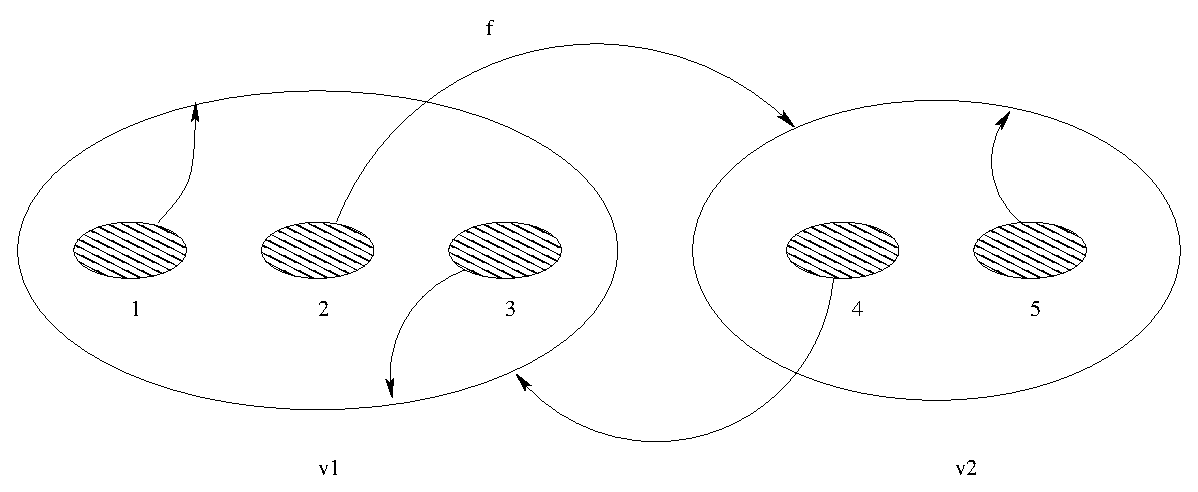
\includegraphics[scale=0.55]{cantor1.eps}
    %  note that the square brace option below is only required
    %  if you intend to produce a list of illustrations
    \caption[Shortened figure caption for the list of illustrations]
      {A Cantor repeller. Long figure captions will be indented left
      and right; short ones will be centred by default.}
    \label{cantor}
\rule[-20pt]{\textwidth}{0.6pt}
\begin{verbatim}
  \begin{figure}
    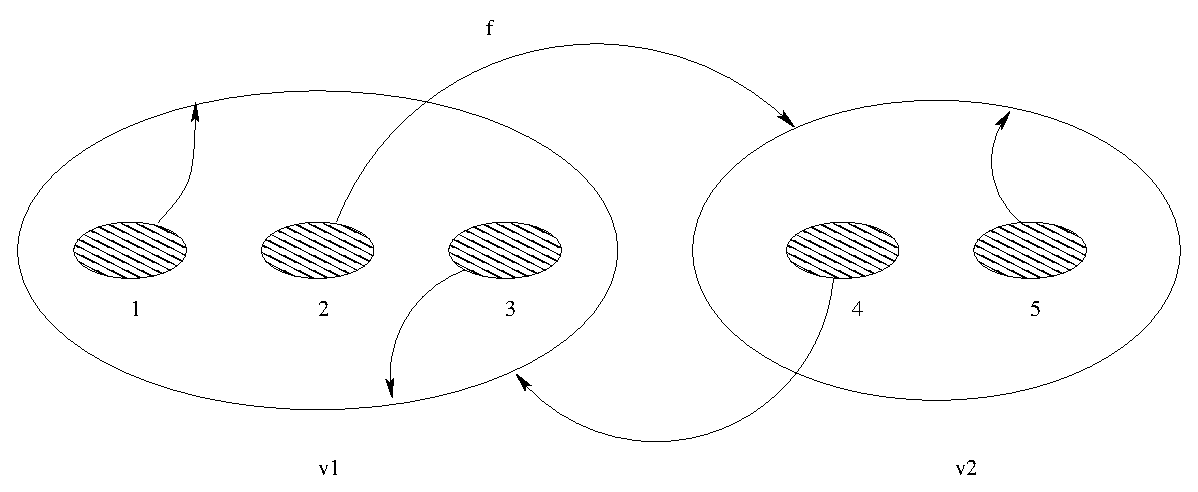
\includegraphics[scale=0.55]{cantor1.eps}
    %  note that the square brace option below is only required
    %  if you intend to produce a list of illustrations
    \caption[Shortened figure caption for the list of illustrations]
      {A Cantor repeller. Long figure captions will be indented left
      and right; short ones will be centred by default.}
    \label{cantor}
  \end{figure}
\end{verbatim}
\rule[20pt]{\textwidth}{0.5pt}
  \end{figure}

\section{Tables}
The \cambridge\ class will cope with most positioning of your tables.
Table captions must be included first, then the label, then the body of the table.
This is illustrated in Table~\ref{sample-table}.
Note that the square brace option below is only required
if you intend to produce a list of tables. You need to use the \verb"minipage"
environment if you have long table captions, or if you have footnotes.

  \begin{table}
    \begin{minipage}{180pt}
    \caption[Shortened table caption for the list of tables]
      {Longer table captions have to be placed inside a minipage,
      otherwise they overhang the table rules.}
    \label{sample-table}
    \addtolength\tabcolsep{2pt}% to stretch columns, if required
      \begin{tabular}{@{}c@{\hspace{25pt}}ccc@{}}
        \hline \hline
        Figure\footnote{\textit{Note:} You must also use a minipage
          environment if you have footnotes.} & $hA$ & $hB$ & $hC$\\
        \hline
        1 & $\exp\left(\pi i\frac58\right)$
          & $\exp\left(\pi i\frac18\right)$ & $0$\\[3pt]
        2 & $-1$    & $\exp\left(\pi i\frac34\right)$ & $1$\\[10pt]
        3 & $-4+3i$ & $-4+3i$ & $\frac74$\\[3pt]
        4 & $-2$    & $-2$    & $\frac54 i$ \\
        \hline \hline
      \end{tabular}
    \end{minipage}
    \rule[-20pt]{\textwidth}{0.5pt}
\begin{verbatim}
  \begin{table}
    \begin{minipage}{180pt}
      %  note that the square brace option below is only required
      %  if you intend to produce a list of tables
    \caption[Shortened table caption for the list of tables]
      {Longer table captions have to be placed inside a minipage,
      otherwise they overhang the table rules.}
    \label{sample-table}
    \addtolength\tabcolsep{2pt}% to stretch columns, if required
      \begin{tabular}{@{}c@{\hspace{25pt}}ccc@{}}
        \hline \hline
        Figure\footnote{\textit{Note:} You must also use a minipage
          environment if you have footnotes.} & $hA$ & $hB$ & $hC$\\
        \hline
        1 & $\exp\left(\pi i\frac58\right)$
          & $\exp\left(\pi i\frac18\right)$ & $0$\\[3pt]
        2 & $-1$    & $\exp\left(\pi i\frac34\right)$ & $1$\\[10pt]
        3 & $-4+3i$ & $-4+3i$ & $\frac74$\\[3pt]
        4 & $-2$    & $-2$    & $\frac54 i$ \\
        \hline \hline
      \end{tabular}
    \end{minipage}
  \end{table}
\end{verbatim}
\rule[20pt]{\textwidth}{0.5pt}
  \end{table}

\subsection{My vertical rules have disappeared}
Vertical rules in tables are not Cambridge house style; {\cambridge}.cls
removes these rules automatically by redefining the \verb"tabular" environment.
Well-organized tables rarely require vertical rules. Where necessary,
grouping can be indicated by the judicious use of extra horizonatal space
(see Section~\ref{addhoriz}). The amended \verb"tabular" also inserts extra
vertical space above and below the horizontal rules produced by \verb"\hline".

Vertical rules can be reinstated, if necessary. Tables will look squashed,
as in the \LaTeX\ book, because the extra vertical space around horizontal
rules will be removed. To reinstate rules globally, add the command
\verb"\reinstaterules" in the preamble; to reinstate rules for an
individual table, place the \verb"\reinstaterules" command
immediately after the relevant \verb"\begin{table}".

The extra space around horizontal rules will also be removed if
you use \verb"array.sty"; you can ignore this effect, because the space
can be reintroduced globally by the typesetters.

\subsection{Adding space between columns}
\label{addhoriz}
You can add space (2pt in this example) between all columns using\linebreak
\verb"\addtolength\tabcolsep{2pt}". If you wanted to expand the space
only between columns~1 and~2, say to~25pt, use
\verb"\begin{tabular}{@{}c@{\hspace{25pt}}ccc@{}}" (see Table~\ref{sample-table}).

\subsection{Adding space between rows}
If you need additional separation between rows (for example,
between rows~2 and~3 in the body of Table~\ref{sample-table}),
adding \verb"[10pt]" immediately after the double backslash at
the end of row~2 will add a 10pt vertical space (the equivalent of
a blank line at this typesize). This method is more controllable
than inserting a horizontal rule.

\section{Landscape figures and tables, using rotating.sty}
Landscape figures and tables are always rotated anticlockwise,
and may be typeset using the \verb"rotating.sty" package with
the \verb"[figuresright]" option. At final make-up stage it is preferable
for landscape pages to fall on verso (left-hand) pages.

In addition to \verb"rotating.sty", include \verb"floatpag.sty" and
the command \verb"\rotfloatpagestyle{empty}". This combination ensures
that headers and footers are removed from the landscape page:
\begin{verbatim}
  \usepackage[figuresright]{rotating}
  \usepackage{floatpag}
  \rotfloatpagestyle{empty}
\end{verbatim}
In some dvi previewers, floats may not appear rotated. If this happens,
you need to convert the dvi file to PostScript or pdf
in order to see the page properly. You can also rotate figures using
the appropriate optional argument in the \verb"\includegraphics" command:
only the illustration is rotated, so running heads are included as usual and captions will
appear at the foot of the figure rather than to the side, both of
which are unsatisfactory in general.

When converting a PostScript file to a pdf file, you may find that
the landscape page comes out upside-down. If this happens, you need
to modify some of the settings in your conversion program.

\subsection{Coding for landscape figures}

Figure~\ref{sidecantor} was produced as follows:
\begin{verbatim}
  \begin{sidewaysfigure}
    \centering
    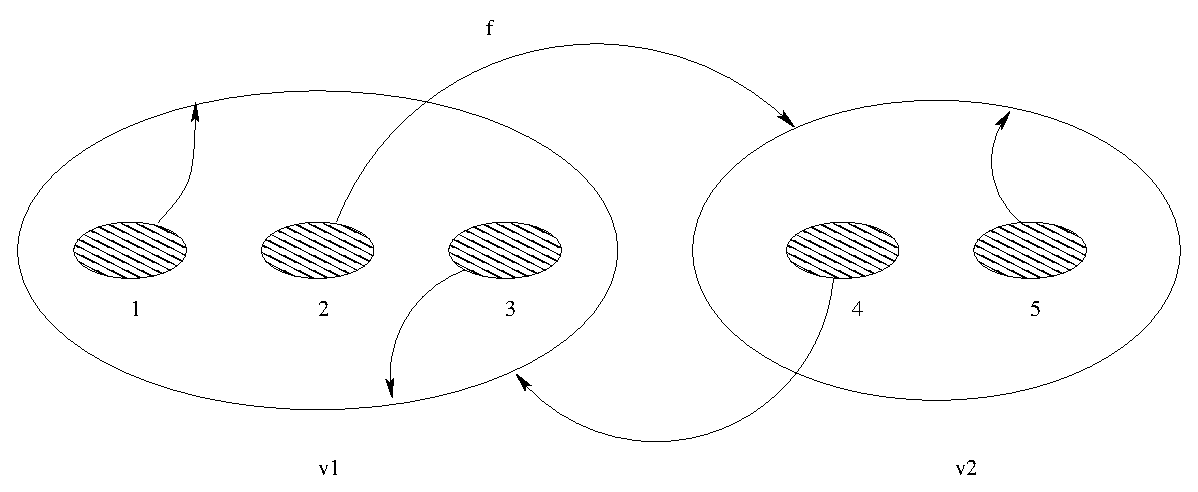
\includegraphics[scale=0.85]{cantor1.eps}
    %  note that the square brace option below is only required
    %  if you intend to produce a list of illustrations
    \caption[Landscape figure]{A Cantor repeller. Figure captions
      will be centred by default.}
    \label{sidecantor}
  \end{sidewaysfigure}
\end{verbatim}
  \begin{sidewaysfigure}
    \centering
    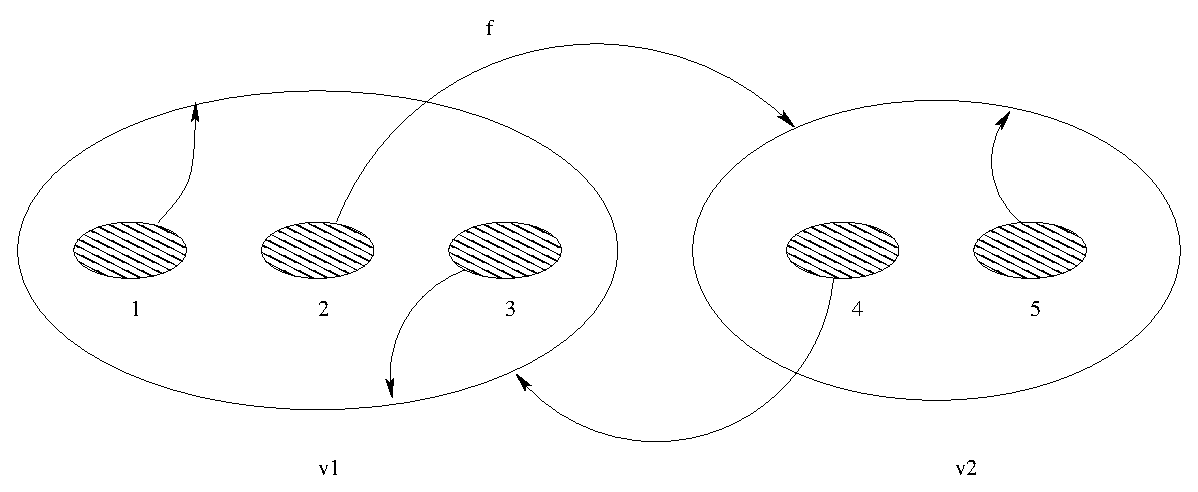
\includegraphics[scale=0.85]{cantor1.eps}
    %  note that the square brace option below is only required
    %  if you intend to produce a list of illustrations
    \caption[Landscape figure]{A Cantor repeller. Figure captions
      will be centred by default.}
    \label{sidecantor}
  \end{sidewaysfigure}


\subsection{Coding for landscape tables}

Table~\ref{sideways} was produced as follows:
%
\begin{smallverbatim}
\begin{sidewaystable}
  \caption[Landscape table]{Grooved ware and beaker features, their finds and
    radiocarbon dates.}
  \label{sideways}
  \addtolength\tabcolsep{-2pt}
  \begin{tabular}{@{}lcccllccccc@{}}
  \hline\hline
  Context & Length & Breadth/  & Depth & Profile & Pottery & Flint & Animal
                                                   & Stone & Other & C14 Dates\\
  && Diameter &&&&& Bones\\[5pt]
  & m & m & m\\
  \hline\\[-5pt]
  \multicolumn{10}{@{}l}{\textbf{Grooved Ware}}\\
  784 & --   & 0.9$\phantom{0}$ &0.18  & Sloping U & P1      & $\times$46
        & $\phantom{0}$$\times$8 && $\times$2 bone & 2150 $\pm$100\,\textsc{bc}\\
  785 & --   & 1.00             &0.12   & Sloping U & P2--4  & $\times$23
                                           & $\times$21 & Hammerstone & -- & --\\
  962 & --   & 1.37             &0.20   & Sloping U & P5--6  & $\times$48
                     & $\times$57 & --& --& 1990 $\pm$80\,\textsc{bc} (Layer 4)\\
  &&&&&&&&&& 1870 $\pm$90\,\textsc{bc} (Layer 1)\\
  983 & 0.83 & 0.73             &0.25   & Stepped U & --     & $\times$18
                                & $\phantom{0}$$\times$8 & -- & Fired clay & --\\
  &&&&&&&&&&\\
  \multicolumn{10}{@{}l}{\textbf{Beaker}}\\
  552 & --   & 0.68             & 0.12  & Saucer    & P7--14 & --           & --
                                                                   & -- &-- &--\\
  790 & --   & 0.60             & 0.25  & U         & P15    & $\times$12   & --
                                                      & Quartzite-lump & -- &--\\
  794 & 2.89 & 0.75             & 0.25  & Irreg.    & P16    & $\phantom{0}$$\times$3
                                                              & -- & -- &-- &--\\
  \hline\hline
  \end{tabular}
\end{sidewaystable}
\end{smallverbatim}
%
\begin{sidewaystable}
  \caption[Landscape table]{Grooved ware and beaker features, their finds and
    radiocarbon dates.}
  \label{sideways}
  \addtolength\tabcolsep{-2pt}
  \begin{tabular}{@{}lcccllccccc@{}}
  \hline\hline
  Context & Length & Breadth/  & Depth & Profile & Pottery & Flint & Animal
                                                   & Stone & Other & C14 Dates\\
  && Diameter &&&&& Bones\\[5pt]
  & m & m & m\\
  \hline\\[-5pt]
  \multicolumn{10}{@{}l}{\textbf{Grooved Ware}}\\
  784 & --   & 0.9$\phantom{0}$ &0.18  & Sloping U & P1      & $\times$46
        & $\phantom{0}$$\times$8 && $\times$2 bone & 2150 $\pm$100\,\textsc{bc}\\
  785 & --   & 1.00             &0.12   & Sloping U & P2--4  & $\times$23
                                           & $\times$21 & Hammerstone & -- & --\\
  962 & --   & 1.37             &0.20   & Sloping U & P5--6  & $\times$48
                     & $\times$57 & --& --& 1990 $\pm$80\,\textsc{bc} (Layer 4)\\
  &&&&&&&&&& 1870 $\pm$90\,\textsc{bc} (Layer 1)\\
  983 & 0.83 & 0.73             &0.25   & Stepped U & --     & $\times$18
                                & $\phantom{0}$$\times$8 & -- & Fired clay & --\\
  &&&&&&&&&&\\
  \multicolumn{10}{@{}l}{\textbf{Beaker}}\\
  552 & --   & 0.68             & 0.12  & Saucer    & P7--14 & --           & --
                                                                   & -- &-- &--\\
  790 & --   & 0.60             & 0.25  & U         & P15    & $\times$12   & --
                                                      & Quartzite-lump & -- &--\\
  794 & 2.89 & 0.75             & 0.25  & Irreg.    & P16    & $\phantom{0}$$\times$3
                                                              & -- & -- &-- &--\\
  \hline\hline
  \end{tabular}%
\end{sidewaystable}

\endinput% Figures and tables
  % 05authored.tex
% 2011/02/28, v3.00 gamma

\chapter{Reference and bibliography lists}
\label{ref}

\section{References and Bibliographies}
Reference lists consist of documents you actually cite in the text; bibliographies
may also list items that are not actually cited so may, for example, contain further reading.
They should be included at the end of the book.
%If you wish to include them at
%the end of chapters instead, or as well, then this can be accommodated with
%a little effort: an example of how to do include references at the ends of
%chapters is given in Section \ref{chapref}.

Reference lists can
be created automatically from a bibliographic database, a \verb".bib" file, or manually; in either instance
you should refer to items in the text using the referencing commands in \LaTeX\
as this will mean your book can be much more easily updated and corrected.

\section{Automatic lists using \textsc{Bib}\upshape{\TeX}}
You will need a \verb".bib" file, a \verb".bst" file that creates a reference
list from that database, and a style file to interpret the commands properly.
For the last, we have chosen to use the natbib package because of its versatility.

First, call in \texttt{natbib.sty}. The bibliographic database for this
guide is called \texttt{percolation.bib};
and we use \texttt{cambridgeauthordate.bst}.
Place the final two commands at the point where you would like the references to appear:
%
\begin{verbatim}
      :
    \usepackage{natbib}
      :
  % \renewcommand{\refname}{Bibliography}
    \bibliography{percolation}
    \bibliographystyle{cambridgeauthordate}
\end{verbatim}
%
Note that by uncommenting the fifth line shown above, you can
change the heading from `References' to `Bibliography'.
Next, \LaTeX\ your book twice. Then run \textsc{Bib}\TeX\ by
executing the command\\[0.5\baselineskip]
\verb"  bibtex "\texttt{\cambridge guide}\\[0.5\baselineskip]
Finally, run your book through \LaTeX\ twice again.
This series of runs will generate a file, the actual reference list,
called \texttt{\cambridge guide.bbl},
which will then be included by \verb"\bibliography{percolation}".

Suppose you have cited 8 entries from the `percolation' database,
e.g. \verb"\citealp{MenshEst}"; \verb"\citealp{Kasymp}"; \verb"\citealp{VGFH}";
\verb"\citealp{HamMaz94}"; \verb"\citealp{HamLower}"; \verb"\citealp{AiBar87}";
\verb"\citealp{MMS}"; and \verb"\citealp{HamAtomBond}";
the output will be just those 8~entries. This guide only cites two items
from the database so only two items are included in the reference list
 (see page~\pageref{refs}).
You can add entries to the list without referring to them
using the \verb"\nocite" command: if you do this the References
should be named as Bibliography.
This guide only cites two items
from the database so only two items are included in the reference list.

\section{Citations using natbib commands}
Here are some of the basic citation commands available with
the natbib package; there are many more if you cannot find what
you need in this list. Bear in mind that Menshikov (1985) or
(Menshikov, 1985) read best, depending on context.\\*[0.5\baselineskip]
\begin{tabular}{@{}ll@{}}
\verb"\citep{MenshEst}"
    & $\rightarrow\enskip$\citep{MenshEst}\\
\verb"\citep[see][p.$\,$34]{MenshEst}"
    & $\rightarrow\enskip$\citep[see][p.$\,$34]{MenshEst}\\
\verb"\citep[e.g.][]{MenshEst}"
    & $\rightarrow\enskip$\citep[e.g.][]{MenshEst}\\
\verb"\citep[Section~2.3]{MenshEst}"
    & $\rightarrow\enskip$\citep[Section~2.3]{MenshEst}\\
\verb"\citep{MenshEst, VGFH}"\\
    & $\hspace{-70pt}\rightarrow\enskip$\citep{MenshEst, VGFH}\\
\verb"\cite{MenshEst, VGFH}"\\
    & $\hspace{-70pt}\rightarrow\enskip$\cite{MenshEst, VGFH}\\
\verb"\citealt{MenshEst}"
    & $\rightarrow\enskip$\citealt{MenshEst}\\
\verb"\cite{MenshEst}"
    & $\rightarrow\enskip$\cite{MenshEst}\\
\verb"\citealp{MenshEst}"
    & $\rightarrow\enskip$\citealp{MenshEst}\\
\verb"\citeauthor{MenshEst}"
    & $\rightarrow\enskip$\citeauthor{MenshEst}\\
\verb"\citeyearpar{MenshEst}"
    & $\rightarrow\enskip$\citeyearpar{MenshEst}\\
\verb"\citeyear{MenshEst}"
    & $\rightarrow\enskip$\citeyear{MenshEst}
\end{tabular}


\subsection{How to change reference entries from author--date to~numbers}
\label{numberedbiblio}

Some authors are used to \verb"\cite{...}" producing a
reference such as~[11] in their manuscripts. If you prefer this style, which
we do not recommend for long lists of references,
use the following option within the natbib package:
\begin{verbatim}
  \usepackage[numbers]{natbib}
\end{verbatim}

\section{Keying in your reference list for an author--date system}
\label{authordatebiblio}

If you are not constructing a list of references from a database,
then the entries need to be keyed as below. Note that if you uncomment
the first line, you can change the heading from `References' to `Bibliography':
%
\begin{smallverbatim}
% \renewcommand{\refname}{Bibliography}
  \begin{thebibliography}{8}
    \expandafter\ifx\csname natexlab\endcsname\relax
      \def\natexlab#1{#1}\fi
    \expandafter\ifx\csname selectlanguage\endcsname\relax
      \def\selectlanguage#1{\relax}\fi

  \bibitem[Aizenman and Barsky, 1987]{AiBar87}
    Aizenman, M., and Barsky, D.~J. 1987.
    Sharpness of the phase transition in percolation models.
    {\em Comm. Math. Phys.}, {\bf 108}, 489--526.

  \bibitem[Hammersley, 1957]{HamLower}
    Hammersley, J.~M. 1957.
    Percolation processes: Lower bounds for the critical probability.
    {\em Ann. Math. Statist.}, {\bf 28}, 790--795.

  \bibitem[Hammersley, 1961]{HamAtomBond}
    Hammersley, J.~M. 1961.
    Comparison of atom and bond percolation processes.
    {\em J. Mathematical Phys.}, {\bf 2}, 728--733.

  \bibitem[Hammersley and Mazzarino, 1994]{HamMaz94}
    Hammersley, J.~M., and Mazzarino, G. 1994.
    Properties of large Eden clusters in the plane.
    {\em Combin. Probab. Comput.}, {\bf 3}, 471--505.

  \bibitem[Kesten, 1990]{Kasymp}
    Kesten, H. 1990.
    Asymptotics in high dimensions for percolation.
    Pages  219--240 of: Grimmett, G.~R., and Welsh, D.~J.~A. (eds),
    {\em Disorder in Physical Systems: A Volume in Honour of John Hammersley}.
    Oxford University Press.

  \bibitem[Menshikov, 1985]{MenshEst}
    Menshikov, M.~V. 1985.
    Estimates for percolation thresholds for lattices in {${\bf R}\sp n$}.
    {\em Dokl. Akad. Nauk SSSR}, {\bf 284}, 36--39.

  \bibitem[Menshikov et~al., 1986]{MMS}
    Menshikov, M.~V., Molchanov, S.~A., and Sidorenko, A.~F. 1986.
    Percolation theory and some applications.
    Pages  53--110 of: {\em Probability theory. Mathematical
    statistics. Theoretical cybernetics, Vol. 24 (Russian)}.
    Akad. Nauk SSSR Vsesoyuz. Inst. Nauchn. i Tekhn. Inform.
    Translated in {\em J. Soviet Math}. {\bf 42} (1988), no. 4,
    1766--1810.

  \bibitem[Vyssotsky et~al., 1961]{VGFH}
    Vyssotsky, V.~A., Gordon, S.~B., Frisch, H.~L., and Hammersley, J.~M. 1961.
    Critical percolation probabilities (bond problem).
    {\em Phys. Rev.}, {\bf 123}, 1566--1567.

  \end{thebibliography}
\end{smallverbatim}

\section{Keying in your reference list for a numbered system}

For this style, you may omit the optional square brace shown
in Section~\ref{authordatebiblio}. Once again, by uncommenting the first line,
you can change the heading from `References' to `Bibliography':
%
\begin{smallverbatim}
% \renewcommand{\refname}{Bibliography}
  \begin{thebibliography}{8}

  \bibitem{AiBar87}
    Aizenman, M., and Barsky, D.~J. 1987.
    Sharpness of the phase transition in percolation models.
    {\em Comm. Math. Phys.}, {\bf 108}, 489--526.
      :
      :
  \bibitem[Vyssotsky et~al., 1961]{VGFH}
    Vyssotsky, V.~A., Gordon, S.~B., Frisch, H.~L., and Hammersley, J.~M. 1961.
    Critical percolation probabilities (bond problem).
    {\em Phys. Rev.}, {\bf 123}, 1566--1567.

  \end{thebibliography}
\end{smallverbatim}

If you add a reference, remember to process \LaTeX\ enough times to get the numbering right in the text.

\section{Including references at the end of chapters}
\label{chapref}

When references are included at the end of chapters, you need to add the command \verb"\chapterreferences", as indicated below. 
In addition, if you wish to change the \textit{References} heading to \textit{References for 
Chapter~\thechapter} (or indeed to something entirely different,
for example \textit{Further Reading}), you can redefine \verb"\refname" as shown:
\begin{verbatim}
  \renewcommand\refname{References for Chapter~\thechapter}
  \chapterreferences
  \bibliography{percolation}\label{refs}
  \bibliographystyle{cambridgeauthordate}
\end{verbatim}

  \renewcommand\refname{References for Chapter~\thechapter}
  \chapterreferences
  \bibliography{percolation}\label{refs}
  \bibliographystyle{cambridgeauthordate}

\section[Including references at the end of chapters \textit{and} at the end of the book]%
  {Including references at the end of chapters \textit{and} at the end of the book
  \sectionmark{References at the end of chapters \textit{and} at the end of the book}}
  \sectionmark{References at the end of chapters \textit{and} at the end of the book}

As illustrated in this guide, add \verb"\bookreferences" immediately before the call 
to the bibliography file. Of course the bibliography file at the end of the book would 
normally be a concatenation of references from the various chapters, but here we are simply using the same one:
\begin{verbatim}
  \renewcommand{\refname}{Bibliography}% if you prefer this heading
  \bookreferences
  \bibliography{percolation}\label{refs}
  \bibliographystyle{cambridgeauthordate}
\end{verbatim}
\endinput% Reference and bibliography lists
  % 06authored.tex
% 2011/02/28, v3.00 gamma

\chapter{Indexes and glossaries}
\label{indexes}

\section{Inserting indexing commands}
You need to code the text so that \LaTeX\ knows what terms to index, and how
to organise them.

If, for example, you have `chocolate cake' in the text, you add this
phrase to the index simply by adding the \verb"\index" command to the source code:
\begin{verbatim}
  ...chocolate cake\index{chocolate cake}
\end{verbatim}
If the text doesn't actually say `chocolate cake', but you want
that in the index, then you should simply type \verb"\index{chocolate cake}" in the source file
at the appropriate point.

\subsection{Subentries}
If your text contained several varieties of cake, you might
also want them listed under `cake' with subentries; to achieve this, use the ! as shown below:
\begin{verbatim}
  ...chocolate cake\index{chocolate cake}\index{cake!chocolate}
  ...lemon cake\index{lemon cake}\index{cake!lemon}
\end{verbatim}
Running the makeindex program (see Section~\ref{makeidx}) will
create an index which contains, in the correct alphabetical order, the following entries:

\vspace{0.5\baselineskip}%
\noindent{\indexsize cake\\
\mbox{}\quad chocolate\\
\mbox{}\quad lemon\\
chocolate cake\\[0.5\baselineskip]
lemon cake\par}

You can also have subsubentries (but there is no support for subsubsubentries):
\begin{verbatim}
  ...Belgian chocolate cake\index{cake!chocolate!Belgian}
\end{verbatim}

\subsection{Page ranges}
If cake appears over several consecutive pages, then the make the first instance:
\begin{verbatim}
  \index{cake|(}
\end{verbatim}
and the final one:
\begin{verbatim}
  \index{cake|)}
\end{verbatim}
When compiled, the index will read (assuming the entries fell on
pages~5 and~10 respectively):\\[0.5\baselineskip]
{\indexsize cake, 5--10}\\[0.5\baselineskip]
The above also works with subentries.

\subsection{Entries without page numbers}
Sometimes you want to add a cross-reference with no page number:
\begin{verbatim}
  ...birthday party\index{cake!orange|see{orange cake}}
\end{verbatim}
will give you:\\[0.5\baselineskip]
{\indexsize cake\\
\mbox{}\quad orange, \textit{see} orange\vadjust{\vspace{3pt}} cake\par}

\subsection{Entries starting with non-alphabetic characters}
If you have index entries in which the first character
is not alphabetical, e.g. \verb"\emph{cake}" or \verb"$\lambda$" you
need to tell \LaTeX\ where to place that word in the final index.
So you would ask for \verb"\emph{cake}" to be sorted as if it
were the word `cake' and \verb"$\lambda$" as if it were the word `lambda'.

The following example shows how to do that
The characters before the \verb"@" symbol in the expression
\verb"lambda@$\lambda$" are for sorting purposes only; what
appears after the symbol is printed in the index. The
character $\lambda$ will appear before lemon cake, since this is what we've requested:
\begin{verbatim}
  ...lemon cake\index{lemon cake}
  ...$\lambda$\index{lambda@$\lambda$}
  ...\emph{cake}\index{cake@\emph{cake}}
\end{verbatim}
The output will be as follows:\\[0.5\baselineskip]
{\indexsize \emph{cake}\\
$\lambda$\\
lemon cake\par}

\section{Creating a single index using makeidx.sty}
\label{makeidx}
The basic \verb"\index" command in \LaTeX\ does not print
anything in its argument but merely `writes' it to a different
file with the extension .idx. (The makeidx programme turns
that into a file with the extension .ind, which is the one in
which all terms are grouped together in alphabetical order,
with all instances and no duplications, i.e. it would
not write 123, 123 against a term in the index.
The .ind file will not change automatically,
even when the .idx file changes: you need to rerun makeidx to change that.) %%BUG: True?

You will need the package makeidx.sty, and the following
commands in the preamble of the root file:\\[0.5\baselineskip]
\verb"  \documentclass{"\texttt{\cambridge}\verb"}"\\
\verb"    \usepackage{makeidx}"\\
\verb"    \makeindex"\\
\verb"    \begin{document}"\\[6.5pt]
%
To generate a single index, normally a subject index, the commands would take the form:
\begin{verbatim}
  \index{diffraction}
  \index{force!hydrodynamic}
  \index{force!interactive}
\end{verbatim}
at the appropriate points in the text.

The command \verb"\printindex" (which outputs the index)
should be placed immediately before the end of the document.
The (optional) \verb"\indextext" command will
insert a phrase below the `Index' chapter heading, across
two columns, the index entries themselves being set in double-column form.

\begin{verbatim}
    \indextext{Page numbers in italics indicate ...}
    \printindex
  \end{document}
\end{verbatim}


Run your files through \LaTeX\ enough times so that the labels, etc.,
are stable. Then execute the command:\\[0.5\baselineskip]
\verb"  makeindex "\texttt{\cambridge test}\\[0.5\baselineskip]
To include the index, you need to run \LaTeX\ one more time.


\section{Creating multiple indexes using multind.sty}
This guide has been prepared using \verb"multind.sty".
This style file redefines the \verb"\makeindex", \verb"\index" and
\verb"\printindex" commands to deal with multiple indexes.

Suppose you want to create an author index and a subject index.
The entries should be in the text as usual, but take the following form:
\begin{verbatim}
  \index{authors}{Young, P.D.F.}
  \index{authors}{Tranah, D.A.}
  \index{authors}{Peterson, K.}
  \index{subject}{diffraction}
  \index{subject}{force!hydrodynamic}
  \index{subject}{force!interactive}
\end{verbatim}
  \index{authors}{Young, P.D.F.}%
  \index{authors}{Tranah, D.A.}%
  \index{authors}{Peterson, K.}%
  \index{subject}{diffraction}%
  \index{subject}{force!hydrodynamic}%
  \index{subject}{force!interactive}%
In the preamble, you need to add the following lines:
\begin{verbatim}
  \usepackage{multind}\ProvidesPackage{multind}
  \makeindex{authors}
  \makeindex{subject}
\end{verbatim}
It is crucial to add the command \verb"\ProvidesPackage{multind}";
this will send a message to the class file to re-style the index into
the \cambridge\ style. You will get a warning in your log file:
\begin{verbatim}
  LaTeX Warning: You have requested package `',
                 but the package provides `multind'.
\end{verbatim}
which can be ignored. At the point where you wish your indexes to appear, you then need the commands:
\begin{verbatim}
  \printindex{authors}{Author index}
  \printindex{subject}{Subject index}
\end{verbatim}
Run your book through \LaTeX\ enough times so that the labels, etc., are stable. Then execute the commands:
\begin{verbatim}
  makeindex authors
  makeindex subject
\end{verbatim}
To include the indexes, you need to run \LaTeX\ one more time.

\section{Warning about index.sty}
This style file also permits multiple indexes.

However, in order to implement \verb"index.sty", it's proved necessary to
modify a number of \LaTeX\ commands seemingly unrelated to indexing,
namely, \verb"\@starttoc", \verb"\raggedbottom", \verb"\flushbottom",
\verb"\addcontents", \verb"\markboth", and \verb"\markright".
Naturally, this could cause incompatibilities between \texttt{index.sty}
and any style files that either redefine these same commands or
make specific assumptions about how they operate.

The redefinition of \verb"\@starttoc" is particularly bad,
since it introduces an incompatibility with the AMS document classes.

For this reason we do not currently recommend using \verb"index.sty".

\enlargethispage{14pt}
\section{Inserting glossary commands}\label{glossary}

You may make use of the glossary.sty style file contained 
within the package http://www.ctan.org/tex-archive/macros/latex/contrib/glossary/.

Briefly, 
you may generate a glossary by inserting the following commands:
%
\begin{verbatim}
\glossary{name={cat},
          description={a domesticated mammal}}

\glossary{name={rabbit},
          description={a rodent, common in the wild or as a pet. Occasionally farmed}}

\glossary{name={dog},
          description={a domesticated mammal, used as a pet or for work purposes}}
\end{verbatim}
where appropriate.
%
\glossary{name={cat},
          description={a domesticated mammal}}

\glossary{name={rabbit},
          description={a rodent, common in the wild or as a pet. Occasionally farmed}}

\glossary{name={dog},
          description={a domesticated mammal, used as a pet or for work purposes}}

You then need to have the following commands in the root file:
\begin{verbatim}
  \usepackage[style=list]{glossary}
  \makeglossary
    :
  \printglossary
\end{verbatim}
(see Appendix~\ref{root} for details). The following example assumes that your 
root file is called tranah.tex. Run the files through \LaTeX, then run the file:
\begin{verbatim}
  makeindex -s tranah.ist -t tranah.glg -o tranah.gls tranah.glo
\end{verbatim}
and finally, run the files through \LaTeX\ again. If you don't want page numbers included (as in this guide)
then add the \verb"number=none" otpional argument, like so:
\begin{verbatim}
  \usepackage[number=none]{glossary}
\end{verbatim}

\endinput
% Indexes
  % 07authored.tex
% 2011/02/28, v3.00 gamma

\chapter{Exercises}
\label{rarities}

\section{Organizing}
Exercises can be handled
in more than one way, as an enunciation or within a list, depending on your style and preference.
They can be scattered through the book, or organised in sets at the end of sections or
chapters, or some combination. But if you mix up styles we strongly recommend
you give the different types different names, for example, Exercises could be
scattered in the text, and Problems could be organised into sets, or vice versa.

\subsection{Scattered through the text --  exer or exer*}
There are two ways of handling exercises scattered through a chapter.
\begin{enumerate}
\item Use amsthm to define an \verb"exer" or \verb"exer*" environment
subject to \verb"\theoremstyle{definition}". See Chapter~\ref{mathchap} for details.
These environments must be defined in the root file for this document.
Exercises created with \verb"exer" are numbered, if at all, in the same sequence as theorems etc.
\item Use the \verb"exerciselist" environment, described below, with a single item.
Exercises created within this environment will be numbered in a
sequence separate from that for theorems etc.

\end{enumerate}

\subsection{At the end of sections -- exerciselist}
The \cambridge\ class file defines the \verb"exerciselist" environment
for setting lists of numbered exercises at the end of sections. These
will not automatically be gathered under a heading, so there will be no  mention of them
in the Table of Contents. Therefore you may wish to list them under a \verb"\subsection"
and set the heading depth appropriately or use the
appropriate \verb"\addcontentsline" command.

There is an option for adding a label such as `Exercise' or `Problem'. The code
\begin{verbatim}
  \begin{exerciselist}[Exercise]
     \item Show that the link between shock formation and
       film rupture is invoked here because of the \ldots
     \item Show that the physical interpretation of \ldots
       \label{physi-ex}
  \end{exerciselist}
\end{verbatim}
will produce
  \begin{exerciselist}[Exercise]
     \item Show that the link between shock formation and
       film rupture is invoked here because of the \ldots
     \item Show that the physical interpretation of \ldots
       \label{physi-ex}
  \end{exerciselist}
Like other numbered environments, individual exercises
(e.g. Exercise~\ref{physi-ex}) can be labeled for automatic cross-referencing.

\subsection{At the end of chapters -- exercises}
If you are gathering all exercises at the end of a given chapter,
use the \verb"exercises" environment rather than \verb"exerciselist". This environment generates an entry
in the table of contents and starts a new unnumbered section and running head. For example,
\begin{verbatim}
  \begin{exercises}
    \item Let the film thickness be $h_0$,
          \begin{equation}
            h=h_0 H{\xi}.
          \label{exerciseeq}
          \end{equation}
          Integrating once, \ldots
    \item Assuming the flow far away from \ldots
  \end{exercises}
\end{verbatim}
will produce (note the mention in the Table of Contents!)
  \begin{exercises}
    \item Let the film thickness be $h_0$,
          \begin{equation}
            h=h_0 H{\xi}.
          \label{exerciseeq}
          \end{equation}
          Integrating once, \ldots
    \item Assuming the flow far away from \ldots
  \end{exercises}
%
If appropriate, you may change the `Exercises' heading to one of the following:
%
\begin{enumerate}[(iii)]
\item `Exercise' -- by using \verb"\begin{exercise}...\end{exercise}"
\item `Problems' -- by using \verb"\begin{problems}...\end{problems}"
\item `Problem' -- by using \verb"\begin{problem}...\end{problem}"
\end{enumerate}
%
For instance,
\begin{verbatim}
  \begin{problems}
    \item By treating $y$ as the independent variable,
          show that the general solution of \ldots
    \item An electrical circuit contains a resistance \ldots
          \label{circuit}
  \end{problems}
\end{verbatim}
will typeset the following:
  \begin{problems}
    \item By treating $y$ as the independent variable,
          show that the general solution of \ldots
    \item An electrical circuit contains a resistance \ldots
          \label{circuit}
  \end{problems}


\endinput
% Exercises

  \backmatter
  \appendix
% if you only have one appendix, use \oneappendix instead of \appendix
  % theorem.tex
% 2011/02/28, v3.00 gamma

\chapter{amsthm commands}
\label{theorem}

You can copy and paste the following code into your root file.
Assuming you have included \verb"amsthm.sty", it will number your theorems,
definitions, etc. in a single sequence within your chapter,
e.g.~Definition~4.1, Lemma~4.2, Lemma~4.3, Proposition~4.4, Corollary~4.5.

\begin{smallverbatim} %don't copy this line!
  \theoremstyle{plain}% default
    \newtheorem{theorem}{Theorem}[chapter]
    \newtheorem{lemma}[theorem]{Lemma}
    \newtheorem{proposition}[theorem]{Proposition}
    \newtheorem{corollary}[theorem]{Corollary}
    \newtheorem{conjecture}[theorem]{Conjecture}

    \newtheorem*{theorem*}{Theorem}
    \newtheorem*{lemma*}{Lemma}
    \newtheorem*{proposition*}{Proposition}
    \newtheorem*{corollary*}{Corollary}
    \newtheorem*{conjecture*}{Conjecture}

  \theoremstyle{definition}
    \newtheorem{definition}[theorem]{Definition}
    \newtheorem{example}[theorem]{Example}
    \newtheorem{prob}[theorem]{Problem}
    \newtheorem{remark}[theorem]{Remark}
    \newtheorem{notation}[theorem]{Notation}
    \newtheorem{exer}[theorem]{Exercise}
    \newtheorem{criterion}[theorem]{Criterion}
    \newtheorem{algorithm}[theorem]{Algorithm}
    \newtheorem{claim}[theorem]{Claim}

    \newtheorem*{definition*}{Definition}
    \newtheorem*{example*}{Example}
    \newtheorem*{prob*}{Problem}
    \newtheorem*{remark*}{Remark}
    \newtheorem*{notation*}{Notation}
    \newtheorem*{exer*}{Exercise}
    \newtheorem*{criterion*}{Criterion}
    \newtheorem*{algorithm*}{Algorithm}
    \newtheorem*{claim*}{Claim}

    \newtheorem*{note}{Note}
    \newtheorem*{summary}{Summary}
    \newtheorem*{acknowledgement}{Acknowledgement}
    \newtheorem*{conclusion}{Conclusion}
\end{smallverbatim} %don't copy this line!

\endinput
  % root.tex
% 2011/06/23, v3.1 gamma

\chapter{The root file for this guide}
\label{root}

\begin{smallverbatim}
% authored_guide.tex
% 2011/06/23, v3.1 gamma
%
% Adapted by Diana Gillooly and David Tranah
% from Ali Woollatt's original documentation for cambridge7A

\NeedsTeXFormat{LaTeX2e}[1996/06/01]

  \documentclass{cambridge7A}
% \documentclass[spanningrule]{../cambridge7A}% option

  \usepackage{natbib}
% \usepackage[numbers]{natbib}% option

  \usepackage[figuresright]{rotating}
  \usepackage{floatpag}
  \rotfloatpagestyle{empty}

% \usepackage{amsmath}% if you are using this package,
                      % it must be loaded before amsthm.sty
  \usepackage{amsthm}
  \usepackage{graphicx}

 \usepackage{txfonts}
% \usepackage[scaled=0.9]{couriers}% use if you're using \tt fonts

% indexes
% uncomment the relevant set of commands

% for a single index
% \usepackage{makeidx}
% \makeindex

% for multiple indexes using multind.sty
  \usepackage{multind}\ProvidesPackage{multind}
  \makeindex{authors}
  \makeindex{subject}

% for glossary entries
  %\usepackage[style=list]{glossary}
  \usepackage[number=none]{glossary}
\makeglossary

% theorem definitions
% see chapter 3 for details
  \theoremstyle{plain}% default
  \newtheorem{theorem}{Theorem}[chapter]
  \newtheorem{lemma}[theorem]{Lemma}
  \newtheorem{proposition}[theorem]{Proposition}
  \newtheorem{corollary}[theorem]{Corollary}
  \newtheorem{conjecture}[theorem]{Conjecture}

  \newtheorem*{theorem*}{Theorem}
  \newtheorem*{lemma*}{Lemma}
  \newtheorem*{proposition*}{Proposition}
  \newtheorem*{corollary*}{Corollary}
  \newtheorem*{conjecture*}{Conjecture}

  \theoremstyle{definition}
  \newtheorem{definition}[theorem]{Definition}
  \newtheorem{example}[theorem]{Example}
  \newtheorem{prob}[theorem]{Problem}
  \newtheorem{remark}[theorem]{Remark}
  \newtheorem{notation}[theorem]{Notation}
  \newtheorem{exer}[theorem]{Exercise}

  \newtheorem*{definition*}{Definition}
  \newtheorem*{example*}{Example}
  \newtheorem*{prob*}{Problem}
  \newtheorem*{remark*}{Remark}
  \newtheorem*{notation*}{Notation}
  \newtheorem*{exer*}{Exercise}

% \hyphenation{docu-ment baseline-skip polar}

% for this documentation, table of contents lists up to subsection level
  \setcounter{tocdepth}{2}

  \newcommand\cambridge{cambridge7A}

% remove the dot and change default for enumerated lists
  \def\makeRRlabeldot#1{\hss\llap{#1}}
  \renewcommand\theenumi{{\rm (\roman{enumi})}}
  \renewcommand\theenumii{{\rm (\alph{enumii})}}
  \renewcommand\theenumiii{{\rm (\arabic{enumiii})}}
  \renewcommand\theenumiv{{\rm (\Alph{enumiv})}}

%%%%%%%%%%%%%%%%%%%%%%%%%%%%%%%%%%%%%

% \includeonly{06authored}

%%%%%%%%%%%%%%%%%%%%%%%%%%%%%%%%%%%%%

\begin{document}

  \title[Subtitle, If You Have One]
    {Preparing Authored Books Using the \cambridge\ Class File}
  \author{Cambridge University Press\\[3\baselineskip]
    This guide was compiled using \hbox{\cambridge.cls \version}\\[\baselineskip]
    The latest version can be downloaded from:
    https://authornet.cambridge.org/information/productionguide/
    LaTeX\_files/\cambridge.zip}

  \bookabstract{This is the guide for authors who are preparing written,
    rather than edited, books.}
  \bookkeywords{\LaTeX; authored books; CUP style; cambridge7A.cls.}

  \frontmatter
  \maketitle
  \tableofcontents
% \listofcontributors

  \include{authored_preface}

  \mainmatter
  \label{partpage}\part{The First Part}
\include{01authored}% Introduction and basic design elements
  \include{02authored}% Numbering and headings
  \include{03authored}% Mathematics
  \include{04authored}% Figures and tables
  \include{05authored}% Reference and bibliography lists
  \include{06authored}% Indexes
  \include{07authored}% Exercises

  \backmatter
  \appendix
% if you only have one appendix, use \oneappendix instead of \appendix
  \include{theorem}
  \include{root}
  \include{appnum}
  \endappendix
  \addtocontents{toc}{\vspace{\baselineskip}}

% the following lines will give you references at the end of the book
  \renewcommand{\refname}{Bibliography}% if you prefer this heading
  \bookreferences % if you already have references at the end of chapters,
                  % you will need this command to start a new \chapter* heading
  \bibliography{percolation}\label{refs}
  \bibliographystyle{cambridgeauthordate}

  \cleardoublepage

% end notes, if you have them
% \theendnotes


% glossary
  \printglossary

% indexes

% for a single index
% \printindex

% for multiple indexes using multind.sty
  \printindex{authors}{Author index}
  \printindex{subject}{Subject index}

\end{document}
\end{smallverbatim}

\endinput


  % appnum.tex
% 2011/02/28, v3.00 gamma

\chapter{Numbering in appendices}
\label{appnum}

In appendices equations are numbered in one sequence by chapter,
but now the chapter `number' is an upper-case letter.
Here are examples.
\begin{equation}\label{einsteinapp}
E = Mc^2 .
\end{equation}
Here are examples of a multiline displays:
\begin{equation}
\left.\begin{array}{rcl}
x &=& a+b\\
y &=& c+d\\
z &=& e+f.
\end{array}\right\}
\end{equation}
\begin{eqnarray}
x&=&a+a+b+b\nonumber\\
&=&2a+b+b\nonumber\\
&=&2a+2b.
\end{eqnarray}

Figures and tables are similarly numbered, via the \verb"\caption", command in the usual way:
\begin{figure}[ht]
\caption{A figure in an appendix.}
\end{figure}
  \endappendix
  \addtocontents{toc}{\vspace{\baselineskip}}

% the following lines will give you references at the end of the book
  \renewcommand{\refname}{Bibliography}% if you prefer this heading
  \bookreferences % if you already have references at the end of chapters,
                  % you will need this command to start a new \chapter* heading
  \bibliography{percolation}\label{refs}
  \bibliographystyle{cambridgeauthordate}

  \cleardoublepage

% end notes, if you have them
% \theendnotes


% glossary
  \printglossary

% indexes

% for a single index
% \printindex

% for multiple indexes using multind.sty
  \printindex{authors}{Author index}
  \printindex{subject}{Subject index}

\end{document}
\end{smallverbatim}

\endinput


  % appnum.tex
% 2011/02/28, v3.00 gamma

\chapter{Numbering in appendices}
\label{appnum}

In appendices equations are numbered in one sequence by chapter,
but now the chapter `number' is an upper-case letter.
Here are examples.
\begin{equation}\label{einsteinapp}
E = Mc^2 .
\end{equation}
Here are examples of a multiline displays:
\begin{equation}
\left.\begin{array}{rcl}
x &=& a+b\\
y &=& c+d\\
z &=& e+f.
\end{array}\right\}
\end{equation}
\begin{eqnarray}
x&=&a+a+b+b\nonumber\\
&=&2a+b+b\nonumber\\
&=&2a+2b.
\end{eqnarray}

Figures and tables are similarly numbered, via the \verb"\caption", command in the usual way:
\begin{figure}[ht]
\caption{A figure in an appendix.}
\end{figure}
  \endappendix
  \addtocontents{toc}{\vspace{\baselineskip}}

% the following lines will give you references at the end of the book
  \renewcommand{\refname}{Bibliography}% if you prefer this heading
  \bookreferences % if you already have references at the end of chapters,
                  % you will need this command to start a new \chapter* heading
  \bibliography{percolation}\label{refs}
  \bibliographystyle{cambridgeauthordate}

  \cleardoublepage

% end notes, if you have them
% \theendnotes


% glossary
  \printglossary

% indexes

% for a single index
% \printindex

% for multiple indexes using multind.sty
  \printindex{authors}{Author index}
  \printindex{subject}{Subject index}

\end{document}
\end{smallverbatim}

\endinput


  % appnum.tex
% 2011/02/28, v3.00 gamma

\chapter{Numbering in appendices}
\label{appnum}

In appendices equations are numbered in one sequence by chapter,
but now the chapter `number' is an upper-case letter.
Here are examples.
\begin{equation}\label{einsteinapp}
E = Mc^2 .
\end{equation}
Here are examples of a multiline displays:
\begin{equation}
\left.\begin{array}{rcl}
x &=& a+b\\
y &=& c+d\\
z &=& e+f.
\end{array}\right\}
\end{equation}
\begin{eqnarray}
x&=&a+a+b+b\nonumber\\
&=&2a+b+b\nonumber\\
&=&2a+2b.
\end{eqnarray}

Figures and tables are similarly numbered, via the \verb"\caption", command in the usual way:
\begin{figure}[ht]
\caption{A figure in an appendix.}
\end{figure}
  \endappendix
  \addtocontents{toc}{\vspace{\baselineskip}}

% the following lines will give you references at the end of the book
  \renewcommand{\refname}{Bibliography}% if you prefer this heading
  \bookreferences % if you already have references at the end of chapters,
                  % you will need this command to start a new \chapter* heading
  \bibliography{percolation}\label{refs}
  \bibliographystyle{cambridgeauthordate}

  \cleardoublepage

% end notes, if you have them
% \theendnotes


% glossary
  \printglossary

% indexes

% for a single index
% \printindex

% for multiple indexes using multind.sty
  \printindex{authors}{Author index}
  \printindex{subject}{Subject index}

\end{document}
